%----------------------------------------------------------------
% [Manual]
%
% [Author]
% Takahiro Misawa   
% [manuscript version]
%   (begin to write on 2015.05.12)
%----------------------------------------------------------------
%
%
\documentclass[a4paper,12pt,openany]{../package/mybook}
%
\usepackage{amsmath, amsfonts, amsthm, amssymb}
\usepackage{graphicx}
\usepackage{color}
\usepackage{bm}
\usepackage{cite}
\usepackage{enumerate}
\usepackage{ascmac}
\usepackage{url}
\usepackage[dvipdfmx]{hyperref}
\def\vec#1{\boldsymbol #1}
\newcommand{\bR}{\mbox{\boldmath $R$}}
\newcommand{\tcy}[1]{\textcolor{black}{#1}}
\newcommand{\tn}[1]{\textcolor{black}{#1}}
\newcommand{\tm}[1]{\textcolor{black}{#1}}
%\newcommand{\tms}[1]{\textcolor{magenta}{\sout{#1}}}
\newcommand{\tr}[1]{\textcolor{red}{#1}}
\newcommand{\trr}[1]{\textcolor{black}{#1}}
\newcommand{\tmm}[1]{\textcolor{black}{#1}}
\newcommand{\tmmm}[1]{\textcolor{black}{#1}}
%\newcommand{\trs}[1]{\textcolor{red}{\sout{#1}}}
\newcommand{\tb}[1]{\textcolor{black}{#1}}
\newcommand{\tbb}[1]{\textcolor{black}{#1}}%\newcommand{\tbs}[1]{\textcolor{blue}{\sout{#1}}}
\newcommand{\tg}[1]{\textcolor{black}{#1}}
\newcommand{\tgg}[1]{\textcolor{black}{#1}}%\newcommand{\tgs}[1]{\textcolor{green}{\sout{#1}}}
\newcommand{\tgf}[1]{\textcolor{black}{#1}}
%
\newcommand{\Ha}{\mathcal{H}}
\newcommand{\mh}{\mathsf{h}}
\newcommand{\mA}{\mathsf{A}}
\newcommand{\mB}{\mathsf{B}}
\newcommand{\mC}{\mathsf{C}}
\newcommand{\mS}{\mathsf{S}}
\newcommand{\mU}{\mathsf{U}}
\newcommand{\mX}{\mathsf{X}}
\newcommand{\sP}{\mathcal{P}}
\newcommand{\sL}{\mathcal{L}}
\newcommand{\sO}{\mathcal{O}}
%
\newcommand{\la}{\langle}
\newcommand{\ra}{\rangle}
\newcommand{\ga}{\alpha}
\newcommand{\gb}{\beta}
\newcommand{\gc}{\gamma}
\newcommand{\gs}{\sigma}
\newcommand{\vk}{{\bm{k}}}
\newcommand{\vq}{{\bm{q}}}
%\newcommand{\vr}{{\bm{r}}}
\newcommand{\vR}{{\bm{R}}}
\newcommand{\vQ}{{\bm{Q}}}
\newcommand{\vga}{{\bm{\alpha}}}
\newcommand{\vgc}{{\bm{\gamma}}}
\newcommand{\Ns}{\mbox{N_{\text{s}}}}
\newcommand{\xx}{\mbox{$x^2-y^2$}}
\newcommand{\zz}{\mbox{$z^2$}}
\newcommand{\HPhi}{ \mathcal{H} \Phi}
\newcommand{\Ham}{\hat{\mathcal{H}}}

\usepackage{ulem}
%
%BINDER STYLE---------------------
%\usepackage[binder]{mythesis}
\usepackage{../package/mythesis}
%---------------------------------
%
%
\bibliographystyle{../bib/elsart-num_mod}
\renewcommand\bibname{References}
%
%---------------------------------
% def and newcommand definition
%
%---------------------------------
%
%
\begin{document}
%================================================================
%  title page
%================================================================
%
\mytitlepage{%
User guide 
}{%
\Huge $\HPhi$ ver. 0.2%
}
%{\large
%{\it \copyright 2015- The University of Tokyo}\\
%{\it  All rights reserved.}
%}
{%
\today
}
%
%================================================================
%  front page
%================================================================
\frontmatter
%Acknowledgments
%  \input{ackn01_en.tex}
%Abstract
%  \input{abst01_en.tex}
%----------------------------------------------------------------
\tableofcontents
\mainmatter
%================================================================
%  main page
%================================================================
  % !TEX root = userguide_en.tex
%----------------------------------------------------------
\chapter{What is ${\HPhi}$?}
\label{Ch:whatishphi}
%----------------------------------------------------------
%----------------------------------------------------------
%----------------------------------------------------------
%----------------------------------------------------------
\section{What is $\HPhi$?}
Comparison between experimental observation and theoretical analysis is a crucial step
in condensed-matter physics research. Temperature dependence of specific heat and
magnetic susceptibility, for example, have been studied to extract nature of low energy
excitations of and magnetic interactions among electrons, respectively, through comparison
with theories such as Landau's Fermi liquid theory and Curie-Weiss law.

For the flexible and quantitative comparison with experimental data, an exact diagonalization
approach~\cite{Dagotto} is one of the most reliable numerical tools without any approximation or
inspiration of genius. For last few decades, a numerical diagonalization package for quantum
spin hamiltonians, TITPACK developed by Prof. Hidetoshi Nishimori in Tokyo Institute of Technology,
has been widely used in the condensed-matter physics community. Nevertheless, limitation of
computational resources had hindered the non-expert users from applying the package to
quantum systems with large number of electrons or spins.

In contrast, recent and rapid development of parallel computing infrastructure opens up new
avenues for user-friendly larger scale diagonalizations up to 18 site Hubbard clusters
or 36 $S$=$1/2$ quantum spins. In addition, recent advances in quantum statistical mechanics ~\cite{Imada1986,FTLanczos,Hams,Sugiura2012}
enable us to calculate finite temperature properties of quantum many-body systems
with computational costs similar to calculations of ground state properties,
which also enables us to compare theoretical results for temperature dependence
of, for example, specific heat and magnetic susceptibility with experimental results quantitatively~\cite{Yamaji2014}.
To utilize the parallel computing infrastructure with narrow bandwidth and distributed-memory
architectures, efficient, user-friendly, and highly parallelized diagonalization packages are highly desirable.

$\HPhi$, a flexible diagonalization package for solving quantum lattice hamiltonians,
has been developed to be such a descendant of the pioneering package TITPACK.
The Lanczos method for calculations of the ground state and a few excited states properties,
and finite temperature calculations based on thermal pure quantum states~\cite{Sugiura2012} are implemented in
the package $\HPhi$, with an easy-to-use and flexible user interface.
By using $\HPhi$, you can analyze a wide range of quantum lattice hamiltonians including
simple Hubbard and Heisenberg models, multi-band extensions of the Hubbard model,
exchange couplings that break SU(2) symmetry of quantum spins such as Dzyaloshinskii-Moriya
and Kitaev interactions, and Kondo lattice models describing itinerant electrons coupled with
quantum spins. $\HPhi$ calculates a variety of physical quantities such as internal energy at zero temperature or finite temperatures, temperature dependence of specific heat, charge/spin structure factors, and so on. A broad spectrum of users including experimental scientists is cordially welcome.

\subsection{License}
The distribution of the program package and the source codes for ${\mathcal H \Phi}$ follow GNU General Public License version 3 (GPL v3). 
\subsection{Copyright}
%{\it \copyright 2015- The University of Tokyo} {\it  All rights reserved.}
{\it \copyright 2015- T. Misawa, K. Yoshimi, M. Kawamura, Y. Yamaji, S. Todo and N. Kawashima.} {\it  All rights reserved.}\\
This software is developed under the support of ``{\it Project for advancement of software usability in materials science }" by The Institute for Solid State Physics, The University of Tokyo. 
%The copyright of this software belongs to The University of Tokyo.
\subsection{Contributors}
\label{subsec:contributors}
This software is developed by following contributors.
\begin{itemize}
\item{ver.0.3 (released at 2016/2/24)}
\item{ver.0.2 (released at 2015/12/28)}
\item{ver.0.1 (released at 2015/10/09)}
\begin{itemize}
	\item{\bf Developers}
	\begin{itemize}
	\item{Takahiro Misawa \\(Department of Applied Physics, The University of Tokyo)}
	\item{Kazuyoshi Yoshimi\\ (The Institute for Solid State Physics, The University of Tokyo)}
	\item{Mitsuaki Kawamura\\ (The Institute for Solid State Physics, The University of Tokyo)}
	\end{itemize}
	\item{\bf Advisers}
	\begin{itemize}
	\item{Youhei Yamaji\\ (Department of Applied Physics, The University of Tokyo)}
	\item{Synge Todo\\ (Department of Physics, The University of Tokyo)}
	\end{itemize}
	\item{\bf Project coordinator}
	\begin{itemize}
	\item{Naoki Kawashima\\ (The Institute for Solid State Physics, The University of Tokyo)}
	\end{itemize}
\end{itemize}
\end{itemize}

\section{Operating environment}
 $\HPhi$ is tested in the following platforms:

\begin{itemize}
\item The supercomputer system-B ``sekirei'' and system-C ``maki'' in ISSP
\item Linux PC + intel compiler
\item Linux PC + gcc
\item Mac + gcc
\end{itemize}

  % !TEX root = userguide_en.tex
%----------------------------------------------------------
\chapter{How to use $\HPhi$?}
\label{Ch:HowTo}

\section{Prerequisite}

$\HPhi$ requires the following packages:
\begin{itemize}
\item C compiler (intel, Fujitsu, GNU, etc. )
\item LAPACK library (intel MKL, Fujitsu TCL, ATLAS, etc.)
\item MPI library (If you do not use MPI, it is not necessary.)
\end{itemize}

\begin{screen}
\Large 
{\bf Tips}
\normalsize

{\bf E. g. / Settings of intel compiler}

When you use the intel compiler, you can use easily scripts attached to the compiler.
In the case of the bash in 64 bit OS, write the following in your \verb|~/.bashrc|:
\begin{verbatim}
source /opt/intel/bin/compilervars.sh intel64
\end{verbatim}
or
\begin{verbatim}
source /opt/intel/bin/iccvars.sh intel64
source /opt/intel/mkl/bin/mklvars.sh
\end{verbatim}

Please read manuals of your compiler/library for more information.

\end{screen}

\section{Installation}
% !TEX root = userguide_en.tex
%----------------------------------------------------------
You can download $\HPhi$ in the following place.\\
\url{https://github.com/QLMS/HPhi/releases}

You can obtain the $\HPhi$ directory by tiping
\begin{verbatim}
$ tar xzvf HPhi-xxx.tar.gz
\end{verbatim}

There are two kind of procedures to install $\HPhi$.

\subsection{Using \texttt{HPhiconfig.sh}}

Please run \verb|HPhiconfig.sh| script in the $\HPhi$ directory as follow
(for ISSP system-B ''sekirei''):
\begin{verbatim}
$ bash HPhiconfig.sh sekirei
\end{verbatim}
Then environmental configuration file \verb|make.sys| is generated in 
\verb|src/| directory.
The command-line argment of \verb|HPhiconfig.sh| is as folows:
\begin{itemize}
\item \verb|sekirei| : ISSP system-B ''sekirei''
\item \verb|maki| : ISSP system-C ''maki''
\item \verb|intel| : intel compiler + Linux PC
\item \verb|mpicc-intel| : intel compiler + MPI (excepting intelMPI) + Linux PC
\item \verb|gcc| : GCC + Linux PC
\item \verb|gcc-mac| : GCC + Mac
\end{itemize}

\verb|make.sys| is as follows (for ISSP-system-B ''sekirei''):
\begin{verbatim}
 CC = mpiicc
 LAPACK_FLAGS = -Dlapack -mkl=parallel 
 FLAGS = -qopenmp  -O3 -xCORE-AVX2 -mcmodel=large -shared-intel -D MPI
 MTFLAGS = -DDSFMT_MEXP=19937 $(FLAGS)
 INCLUDE_DIR=./include
\end{verbatim}
We explatin macros of this file as: 
\begin{itemize}
\item \verb|CC| : The Compilation command (\verb|icc|, \verb|gcc|, \verb|fccpx|)
\item \verb|LAPACK_FLAGS| : Compilation options for LAPACK. \verb|-Dlapack| can not be removed.
\item \verb|FLAGS| : Other compilation options.
  OpenMP utilization option (\verb|-openmp|, \verb|-fopenmp|, \verb|-qopenmp|, etc.)
  must be specified.
  When you use MPI, please set \verb|-D MPI|.
\item \verb|MTFLAGS|, \verb|INCLUDE_DIR| : Options for the Mersenne Twister
  and additional include directory. You do not have to modify them.
\end{itemize}


Then you are ready to compile HPhi.
Please type
\begin{verbatim}
$ make HPhi
\end{verbatim}
and obtain an executable \verb|HPhi| in \verb|src/| directory;
you should add this directory to the \verb|$PATH|.

\subsection{Using \texttt{cmake}}


\begin{screen}
\Large 
{\bf Tips}
\normalsize

You can make a PATH to $\HPhi$ as follows:
\\
\verb|$ export PATH=${PATH}:|\textit{HPhi\_top\_directory}\verb|/src/|
\\
If you keep this PATH, you should write above in \verb|~/.bashrc|
(for \verb|bash| as a login shell)

\end{screen}


\label{Sec:HowToInstall}

\section{Directory structure}
When HPhi-xxx.tar.gz is unzipped, the following directory structure is composed.\\
\\
├──COPYING\\
├──doc/\\
│~~~~~~~├──en/\\
│~~~~~~~├──jp/\\
│~~~~~~~├──userguide\_en.pdf\\
│~~~~~~~└──userguide\_jp.pdf\\
├──HPhiconfig.sh\\
├──samples/\\
│~~~~~~├──Expert/\\
│~~~~~~│~~~~~~├──Hubbard/\\
│~~~~~~│~~~~~~│~~~~~~├─square/\\
│~~~~~~│~~~~~~│~~~~~~│~~~~~~├──*.def\\
│~~~~~~│~~~~~~│~~~~~~│~~~~~~├──output\_FullDiag/\\
│~~~~~~│~~~~~~│~~~~~~│~~~~~~│~~~~~~~~~~└──**.dat\\
│~~~~~~│~~~~~~│~~~~~~│~~~~~~├──output\_Lanczos/\\
│~~~~~~│~~~~~~│~~~~~~│~~~~~~│~~~~~~~~~~└──**.dat\\
│~~~~~~│~~~~~~│~~~~~~│~~~~~~└──output\_TPQ/\\
│~~~~~~│~~~~~~│~~~~~~│~~~~~~~~~~~~~~~~~~└──**.dat\\
│~~~~~~│~~~~~~│~~~~~~└─triangular/\\
│~~~~~~│~~~~~~│~~~~~~~~~~~~└──$\cdots$\\
│~~~~~~│~~~~~~├──Kondo/\\
│~~~~~~│~~~~~~│~~~~~~└─chain/\\
│~~~~~~│~~~~~~│~~~~~~~~~~~~└──$\cdots$\\
│~~~~~~│~~~~~~└──Spin/\\
│~~~~~~│~~~~~~~~~~~~~~~├─HeisenbergChain/\\
│~~~~~~│~~~~~~~~~~~~~~~│~~~~~~└──$\cdots$\\
│~~~~~~│~~~~~~~~~~~~~~~├─HeisenbergSquare/\\
│~~~~~~│~~~~~~~~~~~~~~~│~~~~~~└──$\cdots$\\
│~~~~~~│~~~~~~~~~~~~~~~└─Kitaev/\\
│~~~~~~│~~~~~~~~~~~~~~~~~~~~~~~└──$\cdots$\\
│~~~~~~└──Standard/\\
│~~~~~~~~~~~~~~~~~~├──Hubbard/\\
│~~~~~~~~~~~~~~~~~~│~~~~~~├─square/\\
│~~~~~~~~~~~~~~~~~~│~~~~~~│~~~~~~├──StdFace.def\\
│~~~~~~~~~~~~~~~~~~│~~~~~~│~~~~~~├──output\_FullDiag/\\
│~~~~~~~~~~~~~~~~~~│~~~~~~│~~~~~~│~~~~~~~~~└──**.dat\\
│~~~~~~~~~~~~~~~~~~│~~~~~~│~~~~~~├──output\_Lanczos/\\
│~~~~~~~~~~~~~~~~~~│~~~~~~│~~~~~~│~~~~~~~~~└──**.dat\\
│~~~~~~~~~~~~~~~~~~│~~~~~~│~~~~~~└──output\_TPQ/\\
│~~~~~~~~~~~~~~~~~~│~~~~~~│~~~~~~~~~~~~~~~~~└──**.dat\\
│~~~~~~~~~~~~~~~~~~│~~~~~~└─triangular/\\
│~~~~~~~~~~~~~~~~~~│~~~~~~~~~~~~└──$\cdots$\\
│~~~~~~~~~~~~~~~~~~├──Kondo/\\
│~~~~~~~~~~~~~~~~~~│~~~~~~└─chain/\\
│~~~~~~~~~~~~~~~~~~│~~~~~~~~~~~~└──$\cdots$\\
│~~~~~~~~~~~~~~~~~~└──Spin/\\
│~~~~~~~~~~~~~~~~~~~~~~~~~~~~~~├─HeisenbergChain/\\
│~~~~~~~~~~~~~~~~~~~~~~~~~~~~~~│~~~~~~└──$\cdots$\\
│~~~~~~~~~~~~~~~~~~~~~~~~~~~~~~├─HeisenbergSquare/\\
│~~~~~~~~~~~~~~~~~~~~~~~~~~~~~~│~~~~~~└──$\cdots$\\
│~~~~~~~~~~~~~~~~~~~~~~~~~~~~~~└─Kitaev/\\
│~~~~~~~~~~~~~~~~~~~~~~~~~~~~~~~~~~~~~~~~~~└──$\cdots$\\
└──src/\\
~~~~~~~~~~~~~├──**.c\\
~~~~~~~~~~~~~├──include/\\
~~~~~~~~~~~~~│~~~~~~~└──**.h\\
~~~~~~~~~~~~~└──makefile\_src\\

\section{Basic usage}
$\HPhi$ has two modes; standard mode and expert mode. Here, the basic flows of calculations by standard and expert modes are shown.

\subsection{{\it Standard} mode}

The procedure of calculation through the standard mode is shown as follows:

\begin{enumerate}

\item  Make a directory for a calculation scenario. 

First, you make a working directory for the calculation.

\item  Make input files for standard mode

In the standard mode, you can choose a model (the Heisenberg model, the Hubbard model, etc.) and 
a lattice (the square lattice, the triangular lattice, etc.) from ones provided;
you can specify some parameters (such as the first/second nearest neighbor hopping integrals,
the on-site Coulomb integral, etc.) for them.
Finally, you have to specify the numerical method (such as the Lanczos method) employed in this calculation.
The input file format is described in the Sec. \ref{Ch:HowToStandard}.

\item  Run

Run a executable \verb|HPhi| in terminal by setting option ``\verb|-s|" (or ``\verb|--standard|'') and the name of input file written in previous step.

\begin{itemize}

\item Serial/OpenMP parallel

  \verb|$ |\textit{Path}\verb|/HPhi -s |\textit{Input\_file\_name}

\item MPI parallel/ Hybrid parallel

  \verb|$ mpiexec -np |\textit{number\_of\_processes}\verb| |\textit{Path}\verb|/HPhi -s |\textit{Input\_file\_name}

  When you use a queuing system in workstations or super computers, 
  sometimes the number of processes is specified as an argument for the job-submitting command.
  If you need more information, please refer manuals for your system.

\end{itemize}

\item Watch calculation logs

Log files are outputted in the ``output" folder which is automatically made in the directory for a calculation scenario.
The details of output files are shown in \ref{Sec:outputfile}.

\item Results

If the calculation is finished normally, the result files are outputted in  the ``output" folder. The details of output files are shown in \ref{Sec:outputfile}.

\end{enumerate}

\begin{screen}
\Large 
{\bf Tips}
\normalsize

{\bf The number of threads for OpenMP}

If you specify the number of OpenMP threads for $\HPhi$,
you should set it as follows (in case of 16 threads) before the running:
\begin{verbatim}
export OMP_NUM_THREADS=16
\end{verbatim}

\end{screen}

\subsection{{\it Expert} mode}
The procedure of calculation for expert mode is shown as follows.
 \begin{enumerate}
   \item  Make a directory for a calculation scenario. \\
First, you make a directory named as a calculation scenario (you can attach an arbitrary name to a directory).
   \item  Make input files for expert mode\\
For expert mode,  you should make input files 
for constructing Hamiltonian operators, calculation condition and 
a list file for the filenames of input files (see the file formats shown in  \ref{Ch:HowToExpert}). \\
{\bf Note:} A List file can be easily made by using standard mode.
 \item  Run\\
Run $\HPhi$ in terminal by setting option ``\verb|-e|" (or ``\verb|--expert|'') and a file name of a list file.\\

\begin{itemize}

\item Serial/OpenMPI

  \verb|$ |\textit{Path}\verb|/HPhi -e |\textit{Input\_List\_file\_name}
  
\item MPI/Hybrid

  \verb|$ mpiexec -np |\textit{number\_of\_processes}\verb| |\textit{Path}\verb|/HPhi -e |\textit{Input\_List\_file\_name}

\end{itemize}

\item Under running\\
Log files are outputted in the ``output" folder which is automatically made in the directory for a calculation scenario.
The details of output files are shown in \ref{Sec:outputfile}.

\item Results\\
If the calculation is finished normally, the result files are outputted in  the ``output" folder. The details of output files are shown in \ref{Sec:outputfile}.
\end{enumerate}

  % !TEX root = userguide_en.tex
%----------------------------------------------------------
\chapter{Tutorial}
\label{Ch:model}
\section{{\it Standard} mode}

% !TEX root = userguide_en.tex
\subsection{Heisenberg model}

This tutorial should be performed in 
\begin{verbatim}
samples/Standard/Spin/HeisenbergChain/
\end{verbatim}

The input file, reference outputs, and the redirected standard output are
provided as follows:
\begin{verbatim}
samples/Standard/Spin/HeisenbergChain/StdFace.def
samples/Standard/Spin/HeisenbergChain/output_FullDiag/
samples/Standard/Spin/HeisenbergChain/output_Lanczos/
samples/Standard/Spin/HeisenbergChain/output_TPQ/
samples/Standard/Spin/HeisenbergChain/FullDiag.out
samples/Standard/Spin/HeisenbergChain/Lanczos.out
samples/Standard/Spin/HeisenbergChain/TPQ.out
\end{verbatim}
%
In this case, we treat the one dimensional antiferromagnetic Heisenberg chain
which has a nearest neighbor spin coupling.
\begin{align}
  {\hat H} = J \sum_{i=1}^{N_{\rm site}} {\hat {\boldsymbol S}}_i \cdot {\hat {\boldsymbol S}}_{i+1}
\end{align}

The input file is as follows:
\\
\begin{minipage}{10cm}
\begin{screen}
\begin{verbatim}
L = 16
model = "Spin"
method = "Lanczos"
lattice = "chain lattice"
J = 1.0
2Sz = 0
\end{verbatim}
\end{screen}
\end{minipage}
%
\\
In this tutorial, J and the number of sites are set to 1 (arbitral unit)
and 16 respectively.

\subsubsection{Log output}
{Log messages are outputted to the standard output.
Log files for calculation procedure are made in "output" directory which is automatically created.
In this example, the following files are outputted.\\}
\begin{minipage}{16cm}
\begin{screen}
\begin{verbatim}
CHECK_InterAll.dat     Time_CG_EigenVector.dat  zvo_Lanczos_Step.dat  
CHECK_Memory.dat       WarningOnTransfer.dat    zvo_sz_TimeKeeper.dat
CHECK_Sdim.dat         zvo_TimeKeeper.dat
\end{verbatim}
\end{screen}
\end{minipage}
\\
The details for the outputted files are shown in \ref{Subsec:checkchemi}-\ref{Subsec:timecgeigenv}.
\\
We execute

\hspace{-0.7cm}
\verb|$ |\textit{Path}\verb|/HPhi -s StdFace.def|
\\
and obtain following standard outputs {(a compilation mode is MPI parallel/ Hybrid parallel)}:

\small
\begin{verbatim}
#####  Parallelization Info.  #####

  OpenMP threads : 4
  MPI PEs : 1 


######  Standard Intarface Mode STARTS  ######

  Open Standard-Mode Inputfile ./StdFace.def 

  KEYWORD : l                    | VALUE : 16 
  KEYWORD : model                | VALUE : spin 
  KEYWORD : method               | VALUE : lanczos 
  Skipping a line.
  Skipping a line.
  KEYWORD : lattice              | VALUE : chainlattice 
  KEYWORD : j                    | VALUE : 1.0 
  KEYWORD : 2sz                  | VALUE : 0 

#######  Parameter Summary  #######

                L = 16 
                a = 1.00000     ######  DEFAULT VALUE IS USED  ######
               2S = 1           ######  DEFAULT VALUE IS USED  ######
                h = 0.00000     ######  DEFAULT VALUE IS USED  ######
            Gamma = 0.00000     ######  DEFAULT VALUE IS USED  ######
                D = 0.00000     ######  DEFAULT VALUE IS USED  ######
                J = 1.00000   
               Jz = 1.00000     ######  DEFAULT VALUE IS USED  ######
              Jxy = 1.00000     ######  DEFAULT VALUE IS USED  ######
               Jx = 1.00000     ######  DEFAULT VALUE IS USED  ######
               Jy = 1.00000     ######  DEFAULT VALUE IS USED  ######
               J' = 0.00000     ######  DEFAULT VALUE IS USED  ######
              Jz' = 0.00000     ######  DEFAULT VALUE IS USED  ######
             Jxy' = 0.00000     ######  DEFAULT VALUE IS USED  ######
              Jx' = 0.00000     ######  DEFAULT VALUE IS USED  ######
              Jy' = 0.00000     ######  DEFAULT VALUE IS USED  ######
       LargeValue = 1           ######  DEFAULT VALUE IS USED  ######

         filehead = zvo         ######  DEFAULT VALUE IS USED  ######
      Lanczos_max = 2000        ######  DEFAULT VALUE IS USED  ######
       initial_iv = 1           ######  DEFAULT VALUE IS USED  ######
             nvec = 1           ######  DEFAULT VALUE IS USED  ######
             exct = 1           ######  DEFAULT VALUE IS USED  ######
       LanczosEps = 14          ######  DEFAULT VALUE IS USED  ######
    LanczosTarget = 2           ######  DEFAULT VALUE IS USED  ######
           NumAve = 5           ######  DEFAULT VALUE IS USED  ######
    ExpecInterval = 20          ######  DEFAULT VALUE IS USED  ######
              2Sz = 0  
      ioutputmode = 1           ######  DEFAULT VALUE IS USED  ######

######  Print Expert input files  ######

    zlocspin.def is written.
      zTrans.def is written.
   zInterAll.def is written.
    namelist.def is written.
     calcmod.def is written.
     modpara.def is written.
    greenone.def is written.
    greentwo.def is written.

######  Input files are generated.  ######

  Read File 'namelist.def'.
  Read File 'calcmod.def' for CalcMod.
  Read File 'modpara.def' for ModPara.
  Read File 'zlocspn.def' for LocSpin.
  Read File 'zTrans.def' for Trans.
  Read File 'zInterAll.def' for InterAll.
  Read File 'greenone.def' for OneBodyG.
  Read File 'greentwo.def' for TwoBodyG.

######  Definition files are correct.  ######

  Read File 'zlocspn.def'.
  Read File 'zTrans.def'.
  Read File 'zInterAll.def'.
  Read File 'greenone.def'.
  Read File 'greentwo.def'.

######  Indices and Parameters of Definition files(*.def) are complete.  ######

  MAX DIMENSION idim_max=12870 
  APPROXIMATE REQUIRED MEMORY  max_mem=0.001236 GB 


######  MPI site separation summary  ######

  INTRA process site
    Site    Bit
       0       2
       1       2
       2       2
       3       2
       4       2
       5       2
       6       2
       7       2
       8       2
       9       2
      10       2
      11       2
      12       2
      13       2
      14       2
      15       2

  INTER process site
    Site    Bit

  Process element info
    Process       Dimension   Nup  Ndown  Nelec  Total2Sz   State
          0           12870     8      8      8         0   

   Total dimension : 12870


######  LARGE ALLOCATE FINISH !  ######

  Start: Calculate HilbertNum for fixed Sz. 
  End  : Calculate HilbertNum for fixed Sz. 

  Start: Calculate diagaonal components of Hamiltonian. 
  End  : Calculate diagaonal components of Hamiltonian. 

######  Start: Calculate Lanczos Eigenvalue.  ######

  initial_mode=0 normal: iv = 6437 i_max=12870 k_exct =1 

  LanczosStep  E[1] E[2] E[3] E[4], E_Max / Nsite
  stp = 2 0.7192235936 2.7807764064 xxxxxxxxxx xxxxxxxxx 
  stp = 4 -1.1878294823 0.6833997592 2.1864630296 3.4242789858 0.2140174366 
  stp = 6 -2.4623912732 -0.8925857144 0.5104359160 1.7443963706 0.2277205490 
  stp = 8 -3.5878334190 -2.0969913075 -0.8250723080 0.3369317092 0.2325450330 
\end{verbatim}
\normalsize
( snip )
\small
\begin{verbatim}
  stp = 60 -7.1422963606 -6.8721066784 -6.6965474265 -6.5234070570 0.2499999989 
  stp = 62 -7.1422963606 -6.8721066784 -6.6965474266 -6.5234070573 0.2499999996 
  stp = 64 -7.1422963606 -6.8721066784 -6.6965474266 -6.5234070574 0.2499999999 

######  End  : Calculate Lanczos EigenValue.  ######

######  Start: Calculate Eigenvector.  ######

  Start: Calculate Lanczos Eigenvector.
  End  : Calculate Lanczos Eigenvector.
  Start: Calculate Energy.
  End  : Calculate Energy.

  Accuracy check !!!
  LanczosEnergy = -7.14229636061676e+00 
  EnergyByVec   = -7.14229636061616e+00 
  diff_ene      = 8.50586433832080e-14 
  var           = 9.97303843188625e-14 
  Accuracy of Lanczos vectors is enough.

######  End  : Calculate Eigenvector.  ######

  Start: Calculate one body Green functions.
  End  : Calculate one body Green functions.

  Start: Calculate two bodies Green functions.
  End  : Calculate two bodies Green functions.
\end{verbatim}
\normalsize

In the beginning of this run,
files describing the detail of considered Hamiltonian 
(\verb|zlocspin.def|, \verb|zTrans.def|, \verb|zInterAll.def|, 
\verb|namelist.def|, \verb|calcmod.def|, \verb|modpara.def|)
and files specifying elements of correlation functions
that will be calculated
(\verb|greenone.def|, \verb|greentwo.def|)
are generated.

\begin{screen}
\Large 
{\bf Tips}
\normalsize

In the standard outputs at each even step, 
the quantity of \verb|E_Max / Nsite| column indicates 
the maximum energy per sites
(In this example, it converges to \verb|0.2499999999=0.25|).
In the TPQ calculation, you can set \verb|Largevalue| %to an integer 
larger than \verb|E_Max / Nsite|.

\end{screen}

\subsubsection{Outputs for calculation results}
\begin{description}
\item {\bf Lanczos method}\\
When a calculation by Lanczos method is finished normally, eigenenergies, one-body Green's functions and two-body Green's functions are calculated and outputted to the files, respectively. In this sample, following files are outputted.\\

\begin{minipage}{12cm}
\begin{screen}
\begin{verbatim}
zvo_energy.dat zvo_cisajs.dat 
zvo_cisajscktalt.dat  
\end{verbatim}
\end{screen}
\end{minipage}

For standard mode, all pairs of $\langle n_{i\sigma} \rangle$ are calculated as one-body Green's functions and those of $\langle n_{i\sigma} n_{j\sigma'} \rangle$ are calculated as two-body Green's functions on the basis of the definition files, \verb|greenone.def| and \verb|greentwo.def|. \\
When accuracy of Lanczos vectors is enough, one-body and two-body Green's functions are calculated by eigenvectors obtained by Lanczos method. While accuracy of Lanczos vectors is {\it not} enough, a message ``Accuracy of Lanczos vector is not enough" is outputted to the standard output and one-body and two-body Green's functions are calculated by eigenvectors obtained by CG method.
The details of output files are shown in \ref{subsec:energy.dat}, \ref{Subsec:cgcisajs}, \ref{Subsec:cisajscktalt}.

\item {\bf TPQ method}\\
When \verb|method="TPQ"| is selected in an input file, a calculation by TPQ method is started. After finishing of the calculation normally, following files are outputted, where \%\% is a number of run and \&\& is a number of steps for TPQ method.\\
\begin{minipage}{14cm}
\begin{screen}
\begin{verbatim}
Norm_rand%%.dat SS_rand%%.dat
zvo_cisajs_set%%step&&.dat  
zvo_cisajscktalt_set%%step&&.dat  
\end{verbatim}
\end{screen}
\end{minipage}

In Norm\_rand\%\%.dat, basic informations such as inverse of temperature and a norm of wave function before normalization are outputted with a TPQ step for each number of runs. In SS\_rand\%\%.dat, physical quantities such as inverse of temperature, energy and expected value of square of Hamiltonian are outputted with a TPQ step for each number of runs.  In zvo\_cisajs\_set\%\%step\&\&.dat and zvo\_cisajscktalt\_set\%\%step\&\&.dat, one-body and two-body Green's functions are outputted for each number of a TPQ steps and runs.
The details of these files are shown in \ref{Subsec:normrand}, \ref{Subsec:ssrand}, \ref{Subsec:cgcisajs}, \ref{Subsec:cisajscktalt}.

\item {\bf Full diagonalization method}\\
When \verb|method = "fulldiag"| is selected in an input file, a calculation by Full diagonalization method is started.
After finishing of the calculation normally, following files are outputted, where xx is a number of an eigenstate counting from 0. \\
\begin{minipage}{14cm}
\begin{screen}
\begin{verbatim}
Eigenvalue.dat zvo_cisajs_eigen_xx.dat
zvo_cisajscktalt_eigen_xx.dat  zvo_phys_Nup4_Ndown4.dat
\end{verbatim}
\end{screen}
\end{minipage}

In Eigenvalue.dat, an eigennumber and an eigenvalue are outputted for each lines.
In zvo\_cisajs\_eigen\_xx.dat and zvo\_cisajscktalt\_eigen\_xx.dat, one-body Green's functions and two-body Green's functions are outputted for each eigennumber. 
In zvo\_phys\_Nup4\_Ndown4.dat, physical quantities such as expected values of energy and doublon are outputted. The details of these files are shown in \ref{Subsec:eigenvalue} - \ref{Subsec:cisajscktalt}.


\end{description}

\subsection{Other tutorials}

There are following tutorials in
\verb|samples/Standard/|.

\begin{itemize}
\item The Hubbard model on the two dimensional square lattice

  (\verb|samples/Standard/Hubbard/square/|)
\item The Hubbard model on the two dimensional triangular lattice
  
  (\verb|samples/Standard/Hubbard/triangular/|)
\item The one dimensional Kondo chain

  (\verb|samples/Standard/Kondo/chain/|)
\item The one dimensional antiferromagnetic Heisenberg chain
  
  (\verb|samples/Standard/Spin/HeisenbergChain/HeisenbergChain/|)
\item The antiferromagnetic Heisenberg model on the two dimensional square lattice
  
  (\verb|samples/Standard/Spin/HeisenbergSquare/|)
\item The Kitaev model with 2$\times$3 unit cells to Honeycomb lattice
  
  (\verb|samples/Standard/Spin/Kitaev/|)
\end{itemize}

We can perform these tutorials in the same way to the previous one.

%----------------------------------------------------------
\section{{\it Expert} mode}
For expert mode, following input files are needed
\begin{enumerate}
\item A file list for input files,
\item Files for basic parameters,
\item Files for constructing Hamiltonian,
\item Files for setting output components.
\end{enumerate}
The process after calculation is same as standard mode. In this section, we show the demonstration for one dimensional antiferromagnetic Heisenberg chain model which has a nearest neighbor spin coupling, 
\begin{equation}
H=\sum_{i=0}^{15} J {\bm S}_i\cdot {\bm S}_{i+1},
\end{equation}
where $J=2$, ${\bm S}_{16}={\bm S}_{0}$.\\
We use following input files in samples/Expert/Spin/HeisenbergChain.\\
\begin{minipage}{15cm}
\begin{screen}
\begin{verbatim}
calcmod.def   greentwo.def  namelist.def  zTrans.def
greenone.def  modpara.def   zInterAll.def zlocspn.def
\end{verbatim}
\end{screen}
\end{minipage}

\subsection{A file list for input files}
In namelist.def, kinds of input files and filenames are defined as shown below.
By writing keyword and filenames at each lines, kinds of files are distinguished. The details for namelist.def are shown in  \ref{Subsec:InputFileList}.
\\
\begin{minipage}{15cm}
\begin{screen}
\begin{verbatim}
CalcMod calcmod.def
ModPara modpara.def
LocSpin zlocspn.def
Trans zTrans.def
InterAll zInterAll.def
OneBodyG greenone.def
TwoBodyG greentwo.def
\end{verbatim}
\end{screen}
\end{minipage}

\subsection{Files for basic parameters}
In this subsection, we show the way to set a calculation mode, parameters for calculation and positions of localized spins.
\begin{description}
\item {\bf Setting a calculation mode}\\
Calculation mode is set in a CalcMod file (in this sample file, calcmod.def). The contents of files are shown as below.\\
\begin{minipage}{15cm}
\begin{screen}
\begin{verbatim}
#CalcType = 0:Lanczos, 1:TPQCalc, 2:FullDiag
#CalcMod = 0:Hubbard, 1:Spin, 2:Kondo, 3:HubbardGC, 
4:SpinGC, 5:KondoGC 
CalcType   0
CalcModel   1
\end{verbatim}
\end{screen}
\end{minipage}
~\\
We select a calculation method by CalcType and a target model by CalcModel. In this sample, we set Lanczos method as a calculation method and a target model as a spin system (canonical ensemble). The details of a CalcMod file are shown in \ref{Subsec:calcmod}.\\

\item {\bf Setting parameters for calculation}\\
Parameter for calculation are set in a ModPara file (in this sample, modpara.def). The contents of files are shown as below.\\
\begin{minipage}{15cm}
\begin{screen}
\begin{verbatim}
--------------------
Model_Parameters   0
--------------------
VMC_Cal_Parameters
--------------------
CDataFileHead  zvo
CParaFileHead  zqp
--------------------
Nsite          16   
Ncond          0    
2Sz            0    
Lanczos_max    1000 
initial_iv     12   
nvec           1    
exct           1    
LanczosEps     14   
LanczosTarget  2    
LargeValue     12   
NumAve         5    
ExpecInterval  20 
\end{verbatim}
\end{screen}
\end{minipage}
~\\
In this file, we set parameters for calculation such as a site number, {a total number of conduction electrons,  a total $S_z$} and a number of Lanczos step etc. The details of ModPara file are shown in \ref{Subsec:modpara}.\\

\item {\bf Setting positions of localized spins}\\
Positions {and $S$} of localized spins are defined by a LocSpin file (in this sample, locspn.def). The contents of files are shown as below.\\
\begin{minipage}{15cm}
\begin{screen}
\begin{verbatim}
================================ 
NlocalSpin    16  
================================ 
========i_0LocSpn_1IteElc ====== 
================================ 
    0      1
    1      1
    2      1
    3      1
    4      1
    5      1
...
\end{verbatim}
\end{screen}
\end{minipage}
~\\
When CalcModel in a CalcMod file is set as spin system, all sites automatically treated as localized spins. The details of a LocSpin file is shown in \ref{Subsec:locspn}.
\end{description}

\subsection{Files for constructing Hamiltonian}
After setting basic parameters, we make input files for constructing Hamiltonian. Since calculations are done by the representation of fermion operators in $\HPhi$, we must rewrite spin operator. {For example,  in the case of $S=1/2$, we rewrite the equation by} using the following relation
\begin{align}
S_z^{(i)}&=(c_{i\uparrow}^{\dag}c_{i\uparrow}-c_{i\downarrow}^{\dag}c_{i\downarrow})/2,\\
S_+^{(i)}&=c_{i\uparrow}^{\dag}c_{i\downarrow},\\
S_-^{(i)}&=c_{i\downarrow}^{\dag}c_{i\uparrow}.
\end{align}

\begin{description}
\item {\bf Setting transfer integrals}\\
In a Trans file (in this sample, zTrans.def), we set a transfer part of Hamiltonian,
\begin{align}
H +=-\sum_{ij\sigma_1\sigma2} t_{ij\sigma_1\sigma2}c_{i\sigma_1}^{\dag}c_{j\sigma_2}.
\end{align}
The contents of files are shown as below.\\
\begin{minipage}{15cm}
\begin{screen}
\begin{verbatim}
======================== 
NTransfer       0  
======================== 
========i_j_s_tijs====== 
======================== 
\end{verbatim}
\end{screen}
\end{minipage}
~\\
We can use this term when an electric magnetic field is added in spin system. For example, when an magnetic field is added at a site 1 such as $-0.5 S_z^{(1)}$ { for $S=1/2$}, this term can be rewritten as $-0.5/2(c_{1\uparrow}^{\dag}c_{1\uparrow}-c_{1\downarrow}^{\dag}c_{1\downarrow})$. Thus, the input file becomes as follows.\\
\begin{minipage}{15cm}
\begin{screen}
\begin{verbatim}
======================== 
NTransfer      1   
======================== 
========i_j_s_tijs====== 
======================== 
1 0 1 0 -0.25 0
1 1 1 1 0.25 0
\end{verbatim}
\end{screen}
\end{minipage}
~\\
The details for a Trans file are shown in \ref{Subsec:Trans}.

\item {\bf Setting general two-body interactions}\\
In an InterAll file (in this sample, zInterall.def), we set a general two-body interaction part of Hamiltonian,
\begin{equation}
H+=\sum_{i,j,k,l}\sum_{\sigma_1,\sigma_2, \sigma_3, \sigma_4}
I_{ijkl\sigma_1\sigma_2\sigma_3\sigma_4}c_{i\sigma_1}^{\dagger}c_{j\sigma_2}c_{k\sigma_3}^{\dagger}c_{l\sigma_4}.
\end{equation}
The contents of files are shown as below.\\
\begin{minipage}{16cm}
\begin{screen}
\begin{verbatim}
====================== 
NInterAll      96  
====================== 
========zInterAll===== 
====================== 
    0     0     0     0     1     0     1     0   0.500000  0.000000
    0     0     0     0     1     1     1     1  -0.500000  0.000000
    0     1     0     1     1     0     1     0  -0.500000  0.000000
    0     1     0     1     1     1     1     1   0.500000  0.000000
    0     0     0     1     1     1     1     0   1.000000  0.000000
    0     1     0     0     1     0     1     1   1.000000  0.000000
...
\end{verbatim}
\end{screen}
\end{minipage}
~\\
Here, we explain an interaction between a site $i$ and a site $j$ {in the case of $S=1/2$}, for simplicity. Using fermion operators, interaction terms for spin operators can be rewritten as
\begin{align}
H_{i,i+1}&=J(S_x^{(i)}S_x^{(i+1)}+S_y^{(i)}S_y^{(i+1)}+S_z^{(i)}S_z^{(i+1)}) \nonumber\\
&=J \left( \frac{1}{2}S_+^{(i)}S_-^{(i+1)}+\frac{1}{2}S_-^{(i)}S_+^{(i+1)}+S_z^{(i)}S_z^{(i+1)} \right) \nonumber\\
&=J \left[ \frac{1}{2}c_{i\uparrow}^{\dag}c_{i\downarrow}c_{i+1\downarrow}^{\dag}c_{i+1\uparrow}+\frac{1}{2}c_{i\downarrow}^{\dag}c_{i\uparrow}c_{i+1\uparrow}^{\dag}c_{i+1\downarrow}+\frac{1}{4}(c_{i\uparrow}^{\dag}c_{i\uparrow}-c_{i\downarrow}^{\dag}c_{i\downarrow})(c_{i+1\uparrow}^{\dag}c_{i+1\uparrow}-c_{i+1\downarrow}^{\dag}c_{i+1\downarrow}) \right]. \nonumber 
\end{align}
Thus, the interaction $S_z^{(i)}S_z^{(i+1)}$ for $J=2$ can be written as \\
\begin{minipage}{16cm}
\begin{screen}
\begin{verbatim}
    i     0     i     0    i+1     0    i+1     0   0.500000  0.000000
    i     0     i     0    i+1     1    i+1     1  -0.500000  0.000000
    i     1     i     1    i+1     0    i+1     0  -0.500000  0.000000
    i     1     i     1    i+1     1    i+1     1   0.500000  0.000000
\end{verbatim}
\end{screen}
\end{minipage}
~\\
in the format of an InterAll file. The other terms can be written as below.\\
\begin{minipage}{16cm}
\begin{screen}
\begin{verbatim}
    i     0     i     1    i+1     1    i+1     0   1.000000  0.000000
    i     1     i     0    i+1     0    i+1     1   1.000000  0.000000
\end{verbatim}
\end{screen}
\end{minipage}
~\\
There are other file formats for constructing Hamiltonian. The details for input formats of two-body interactions are shown in \ref{Subsec:interall}-\ref{Subsec:pairlift}.

\end{description}

\subsection{Setting output components}
In OneBodyG and TwoBodyG files, calculating components for one-body and two-body Green's functions are defined, respectively. 
\begin{description}
\item {\bf Setting calculating components for one-body Green's functions}\\
In a OneBodyG file (in this sample, greenone.def), calculating components for $\langle c_{i\sigma_1}^{\dag}c_{j\sigma_2} \rangle$ are defined. The contents of files are shown as below.\\
\begin{minipage}{15cm}
\begin{screen}
\begin{verbatim}
===============================
NCisAjs         32
===============================
======== Green functions ======
===============================
    0     0     0     0
    0     1     0     1
    1     0     1     0
    1     1     1     1
    2     0     2     0
...
\end{verbatim}
\end{screen}
\end{minipage}
~\\
The details for input formats of a OneBodyG file are shown in \ref{Subsec:onebodyg}.
\item {\bf Setting calculating components for two-body Green's functions}\\
In a TwoBodyG file (in this sample, greentwo.def), calculating components for $\langle c_{i\sigma_1}^{\dag}c_{j\sigma_2}c_{k\sigma_3}^{\dag}c_{l\sigma_4} \rangle$ are defined. The contents of files are shown as below.\\
\begin{minipage}{15cm}
\begin{screen}
\begin{verbatim}
=============================================
NCisAjsCktAltDC       1024
=============================================
======== Green functions for Sq AND Nq ======
=============================================
    0     0     0     0     0     0     0     0
    0     0     0     0     0     1     0     1
    0     0     0     0     1     0     1     0
    0     0     0     0     1     1     1     1
    0     0     0     0     2     0     2     0
    ...
\end{verbatim}
\end{screen}
\end{minipage}
~\\
The details for input formats of a TwoBodyG file are shown in \ref{Subsec:twobodyg}.
\end{description}

\subsection{Running}
After making all input files above, we ready to run a program. For expert mode, we must set an option ``-e" and a file name list (in this sample, namelist.def) as arguments to run $\HPhi$.\\
\verb|$ |\textit{Path}\verb|/HPhi -e namelist.def|\\
The process after calculating is same as that of standard mode.

\subsection{Other tutorials}

There are following tutorials in \verb|samples/Expert/|.

\begin{itemize}
\item The Hubbard model on the two dimensional square lattice

  (\verb|samples/Expert/Hubbard/square/|)
\item The Hubbard model on the two dimensional triangular lattice
  
  (\verb|samples/Expert/Hubbard/triangular/|)
\item The one dimensional Kondo chain

  (\verb|samples/Expert/Kondo/chain/|)
\item The one dimensional antiferromagnetic Heisenberg chain
  
  (\verb|samples/Expert/Spin/HeisenbergChain/HeisenbergChain/|)
\item The antiferromagnetic Heisenberg model on the two dimensional square lattice
  
  (\verb|samples/Expert/Spin/HeisenbergSquare/|)
      
\item The Kitaev model with 2$\times$3 unit cells to Honeycomb lattice

  (\verb|samples/Expert/Spin/Kitaev/|)

\end{itemize}

We can perform these tutorials in the same way to the previous one.

\newpage
\section{Making input files for {\it Expert} mode}
This mode is to make input files for {\it Expert} mode. A set of input files made by this mode gives a model provided in {\it Standard} mode.
The usage is shown as below.
\begin{enumerate}
\item{Make an input file for {\it Standard} mode.}
\item{Setting an option ``-sdry" and an input file (in this example, StdFace.def), run $\HPhi$.}\\
\verb|$ |\textit{Path}\verb|/HPhi -sdry StdFace.def|

In this case, you should not use MPI parallelization (\verb|mpirun|, \verb|mpiexec|, etc.).
\item{Following files are made as input files for {\it Expert} mode in the present working directory.}\\
\begin{minipage}{12cm}
\begin{screen}
\begin{verbatim}
calcmod.def   greentwo.def  namelist.def  zTrans.def
greenone.def  modpara.def   zInterAll.def zlocspn.def
\end{verbatim}
\end{screen}
\end{minipage}
\end{enumerate}

  % !TEX root = userguide_en.tex
%----------------------------------------------------------
\chapter{File specification}
\label{Ch:HowToStandard}
%----------------------------------------------------------
\section{Input files for {\it Standard} mode}

% !TEX root = userguide_en.tex
%----------------------------------------------------------
An example of an input file for the standard mode is as follows:

\begin{minipage}{10cm}
\begin{screen}
\begin{verbatim}
W = 2
 L = 4
 model = "spin"
 method = "Lanczos"

 lattice = "triangular lattice"
//mu = 1.0
// t = -1.0
// t' = -0.5
// U = 8.0
//V = 4.0
//V'=2.0
J = -1.0
J'=-0.5
// nelec = 8
2Sz = 0
\end{verbatim}
\end{screen}
\end{minipage}
~\\
~\\
~\\
{\bf Basic rules for input files}
\begin{itemize}
\item In each line, there is a set of a keyword (before an ``\verb|=|") and a parameter(after an ``\verb|=|"); 
  they are separated by ``\verb|=|".
\item You can describe keywords in a random order.
\item Empty lines and lines beginning with a ``\verb|//|''(comment outs) are skipped.
\item Upper- and lowercase are not distinguished.
  Double quotes and blanks are ignored.
\item There are three types of parameters.\\ 
  1.~Parameters that must be specified~(if not, $\HPhi$ will stop with error messages),\\ 
  2.~Parameters that it is not necessary to specified~(if not specified, default values are used),\\
  3.~Parameters that must not be specified~(if specified, $\HPhi$ will stop with error messages).\\
  An example of type 3 is the transfer $t$ parameter for the Heisenberg spin system. 
  If you choose ``model=spin", you should not specify ``$t$".
\end{itemize}

We explain each keyword as follows.

\subsection{Parameters for the type of calculation}

\begin{itemize}

\item \verb|model|

{\bf Type :} String (hoose from \verb|"Fermion Hubbard"|, \verb|"Spin"|, \verb|"Kondo Lattice"|, 
\verb|"Fermion HubbardGC"|, \verb|"SpinGC"|, \verb|"Kondo LatticeGC"|, \verb|"SpinGCCMA"|)\footnote{GC=Grand Canonical}

{\bf Description :} The target model is specified with this parameter;
the expressions above denote the canonical ensemble of the Fermion in the Hubbard model
\begin{align}
H = -\mu \sum_{i \sigma} c^\dagger_{i \sigma} c_{i \sigma} 
- \sum_{i \neq j \sigma} t_{i j} c^\dagger_{i \sigma} c_{j \sigma} 
+ \sum_{i} U n_{i \uparrow} n_{i \downarrow}
+ \sum_{i \neq j} V_{i j} n_{i} n_{j},
\label{fml4_1_hubbard}
\end{align}
the canonical ensemble in the Spin model($\{\sigma_1, \sigma_2\}={x, y, z}$)
\begin{align}
H &= -h \sum_{i} S_{i z} - \Gamma \sum_{i} S_{i x} + D \sum_{i} S_{i z} S_{i z}
\nonumber \\
&+ \sum_{i j, \sigma_1}J_{i j \sigma_1} S_{i \sigma_1} S_{j \sigma_1}+ \sum_{i j, \sigma_1 \neq \sigma_2} J_{i j \sigma_1 \sigma_2} S_{i \sigma_1} S_{j \sigma_2} ,
\label{fml4_1_spin}
\end{align}
the canonical ensemble in the Kondo lattice model
\begin{align}
H = - \mu \sum_{i \sigma} c^\dagger_{i \sigma} c_{i \sigma} 
- t \sum_{\langle i j \rangle \sigma} c^\dagger_{i \sigma} c_{j \sigma} 
+ \frac{J}{2} \sum_{i} \left\{
S_{i}^{+} c_{i \downarrow}^\dagger c_{i \uparrow}
+ S_{i}^{-} c_{i \uparrow}^\dagger c_{i \downarrow}
+ S_{i z} (n_{i \uparrow} - n_{i \downarrow})
\right\},
\label{fml4_1_kondo}
\end{align}
the grand canonical ensemble of the Fermion in the Hubbard model [Eqn. (\ref{fml4_1_hubbard})],
the grand canonical ensemble in the Spin model [Eqn. (\ref{fml4_1_spin})],
and
the grand canonical ensemble in the Kondo lattice model [Eqn. (\ref{fml4_1_kondo})],
respectively.

When \verb|model="SpinGCCMA"|,
by using a more efficient algorithm\footnote{Y. Yamaji \textit{et. al.}, manuscript in preparation.}, 
$\HPhi$ calculates a system that is the same as \verb|"SpinGC"|.
However, supported models and MPI processes are highly limited.
See \verb|"Lattice"| section.

\item \verb|method|
  
{\bf Type :} String (choose from \verb|"Lanczos"|, \verb|"TPQ"|, \verb|"Full Diag"|, \verb|"CG"|)

{\bf Description :} The calculation type is specified with this parameter;
the above expressions above denote 
the single eigenstate calculation by using the Lanczos method,
at the finite-temperature by using the thermally pure quantum state,
the full diagonalization method,
and the multiple eigenstates calculation by using the LOBCG method
\cite{doi:10.1137/S1064827500366124,transactionJSCES2006},
respectively.

The scheme employed for the spectrum calculation is also specified with this parameter.
If \verb|"CG"| is chosen, the shifted bi-conjugate gradient method \cite{Frommer2003}
together with the seed-switch technique \cite{doi:10.1143/JPSJ.77.114713} is employed
with the help of the $K\omega$ library \cite{komega}.

\item \verb|lattice|

{\bf Type :} String (choose from \verb|"Chain Lattice"|, \verb|"Square Lattice"|, 
\verb|"Triangular Lattice"|, \verb|"Honeycomb Lattice"|, \verb|"Ladder"|, \verb|"Kagome"|)

{\bf Description :} The lattice shape is specified with this parameter;
the expressions above denote
the one-dimensional chain lattice (Fig. \ref{fig_chap04_1_lattice}(a)), 
the two-dimensional square lattice (Fig. \ref{fig_chap04_1_lattice}(b)),
the two-dimensional triangular lattice (Fig. \ref{fig_chap04_1_lattice}(c)),
the two-dimensional anisotropic honeycomb lattice (Fig. \ref{fig_chap04_1_honeycomb}),
the ladder lattice (Fig. \ref{fig_ladder}),
and
the Kagome Lattice(Fig. \ref{fig_kagome})
respectively.

In \verb|method="SpinGCCMA"|,
only \verb|"Chain Lattice"|, \verb|"Honeycomb Lattice"|, 
\verb|"Ladder"|, and \verb|"Kagome"| are supported.
The limits of $L$, $W$, and the number of MPI processes ($N_{\rm proc}$) are as follows:

\begin{itemize}

  \item \verb|"Chain Lattice"|

    $L = 8n$ (where $n$ is an integer number under the condition  $n\geq1$),
    $N_{\rm proc} \leq 2(L=8)$, $N_{\rm proc} \leq 2^{L/2-2}(L>8)$.
    
  \item \verb|"Honeycomb Lattice"|

    $W=3, L \geq 2$, $N_{\rm proc} \leq 2(L=2)$, $N_{\rm proc} \leq 64(L>2)$.

  \item \verb|"Ladder"|

    $W=2, L = 2n$ (where $n$ is an integer number under the condition  $n\geq4$),
    $N_{\rm proc} \leq 2^{L-4}$.

  \item \verb|"Kagome"|

    $W=3, L \geq 2$, $N_{\rm proc} \leq 1(L=2)$, $N_{\rm proc} \leq 512(L>2)$.

\end{itemize}

\begin{figure}[!tbhp]
  \begin{center}
    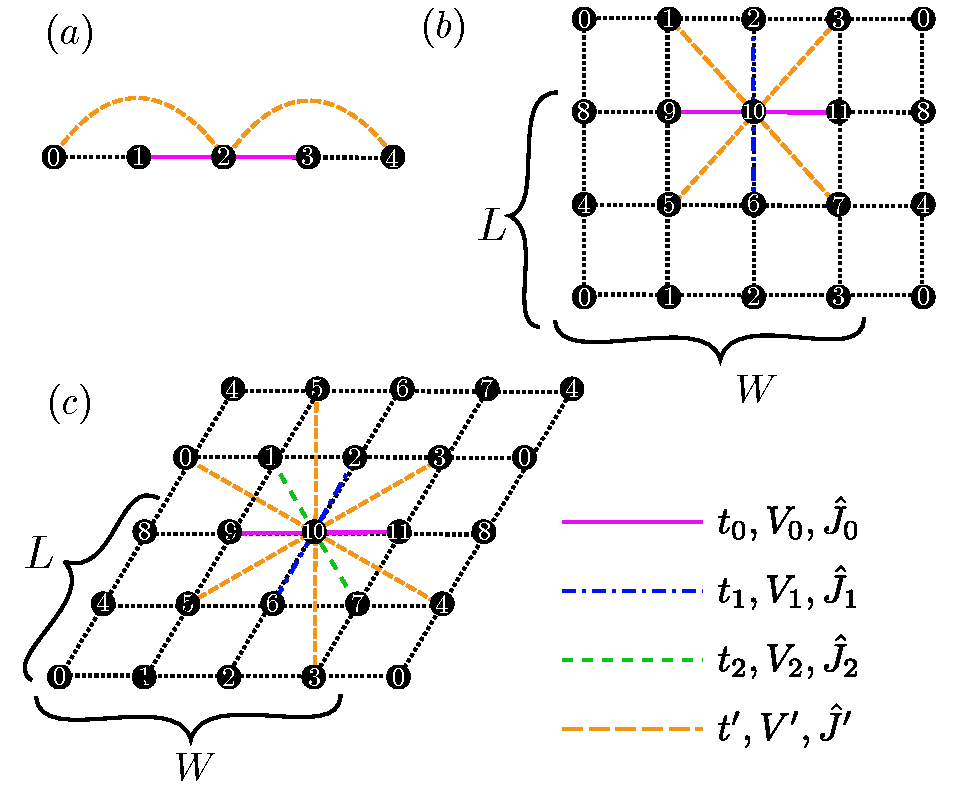
\includegraphics[width=8cm]{../figs/chap04_1_lattice.pdf}
    \caption{Schematic illustration of
      (a) one-dimensional chain lattice, 
      (b) two-dimensional square lattice, and 
      (c) two-dimensional triangular lattice.
      They have $t$, $V$, and $J$ as the nearest neighbor hopping, an offsite Coulomb integral, 
      and a spin-coupling constant, respectively (magenta solid lines);
      they also have $t'$, $V'$, and $J'$ as the next nearest neighbor hopping, offsite Coulomb integral, 
      and spin-coupling constant, respectively (green dashed line).
    }
    \label{fig_chap04_1_lattice}
  \end{center}
\end{figure}

\begin{figure}[!tbhp]
  \begin{center}
    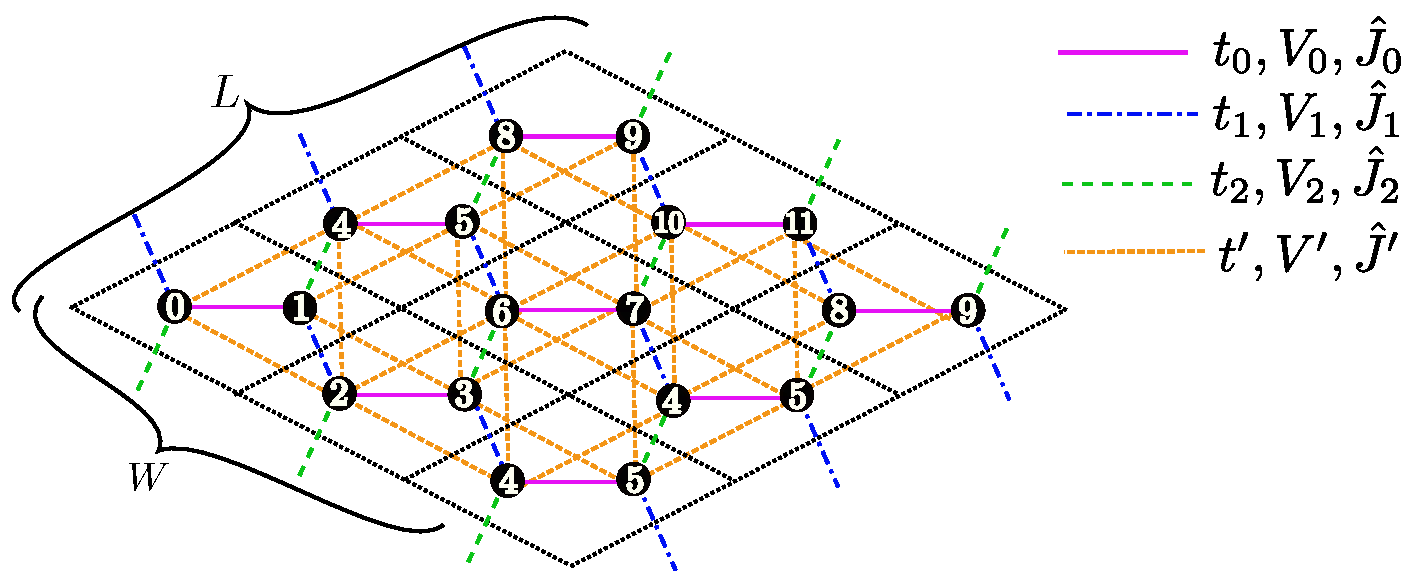
\includegraphics[width=15cm]{../figs/chap04_1_honeycomb.pdf}
    \caption{Schematic illustration of the anisotropic honeycomb lattice.
      The nearest neighbor 
      hopping integral, spin coupling, and offsite Coulomb integral
      depend on the bond direction.
      Those between the second nearest neighbor sites are not supported.
    }
    \label{fig_chap04_1_honeycomb}
  \end{center}
\end{figure}

\begin{figure}[!tbhp]
  \begin{center}
    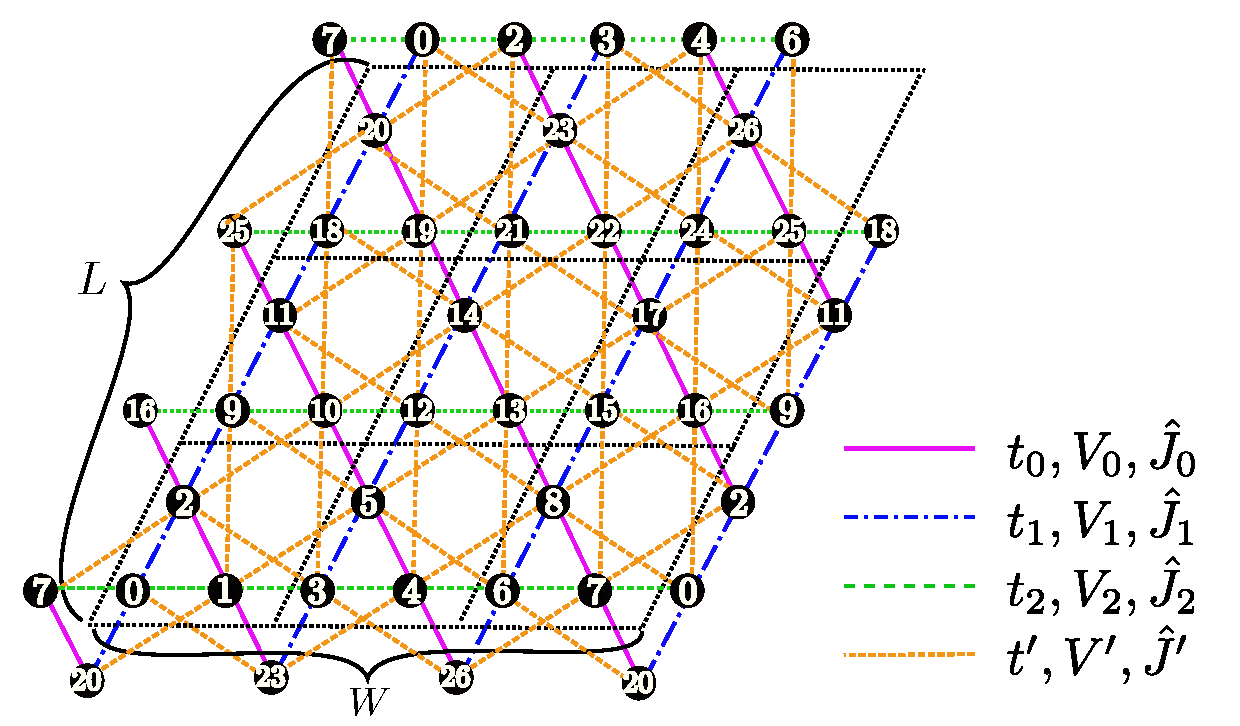
\includegraphics[width=10cm]{../figs/kagome.pdf}
    \caption{Schematic illustration of the Kagome lattice.
    }
    \label{fig_kagome}
  \end{center}
\end{figure}

\begin{figure}[!tbhp]
  \begin{center}
    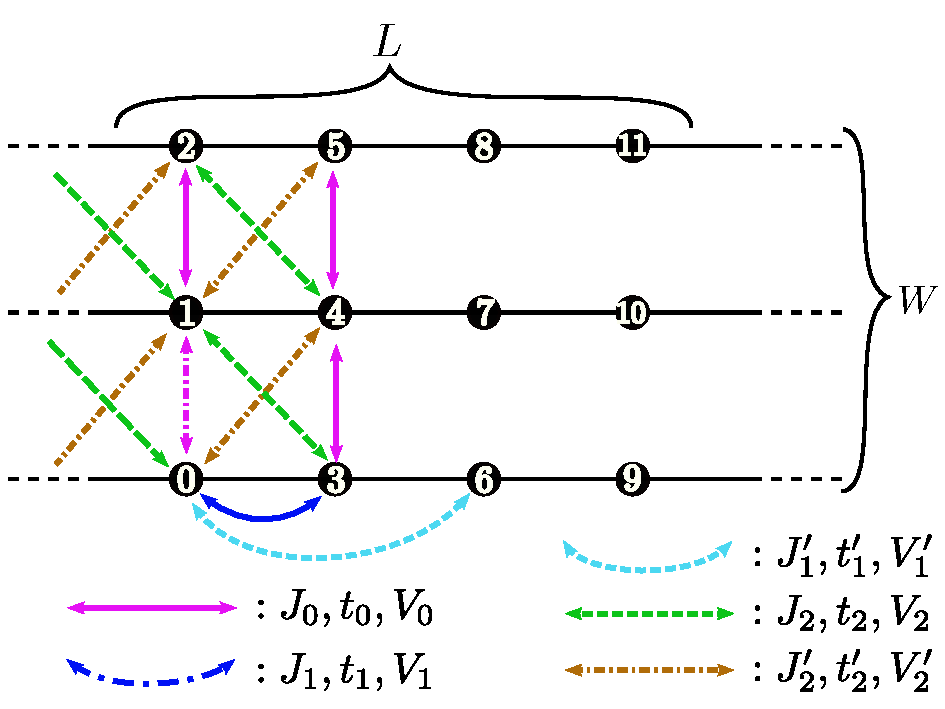
\includegraphics[width=10cm]{../figs/ladder.pdf}
    \caption{Schematic illustration of the ladder lattice.
    }
    \label{fig_ladder}
  \end{center}
\end{figure}


\end{itemize}

\subsection{Parameters for the lattice}

\subsubsection{Chain [Fig. \ref{fig_chap04_1_lattice}(a)]}

\begin{itemize}

\item \verb|L|

{\bf Type :} Integer

{\bf Description :} The length of the chain is specified 
with this parameter.

\end{itemize}

\subsubsection{Ladder (Fig. \ref{fig_ladder})}

\begin{itemize}

\item \verb|L|

{\bf Type :} Integer

{\bf Description :} The length of the ladder is specified 
with this parameter.

\item \verb|W|

{\bf Type :} Integer

{\bf Description :} The number of the ladder is specified 
with this parameter.

\end{itemize}

\begin{figure}[!tbhp]
  \begin{center}
    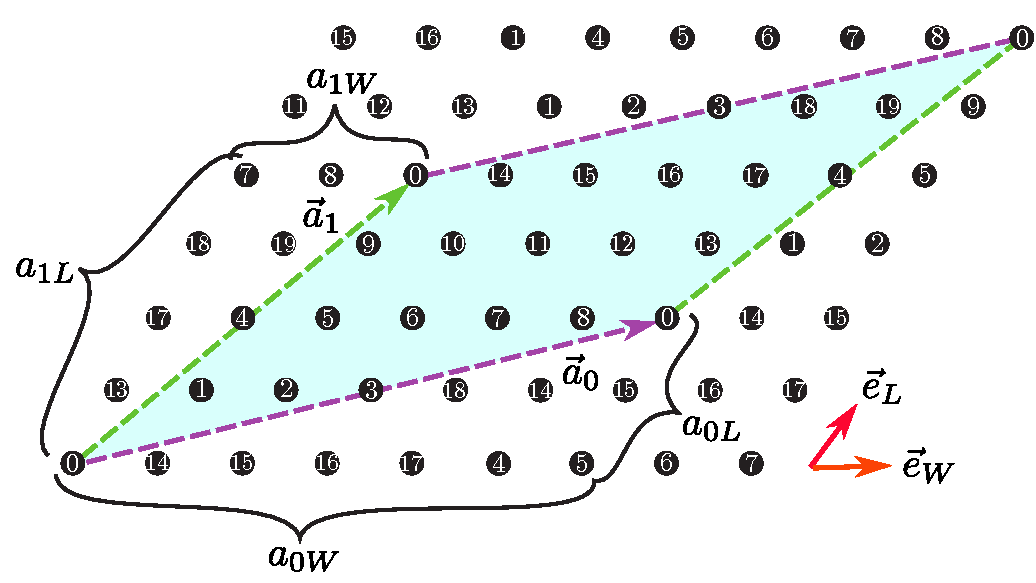
\includegraphics[width=15cm]{../figs/chap04_1_unitlattice.pdf}
    \caption{Shape of the numerical cell 
      when ${\vec a}_0 = (6, 2), {\vec a}_1 = (2, 4)$
      in the triangular lattice.
      The region surrounded by 
      ${\vec a}_0$ (magenta dashed arrow) and ${\vec a}_1$ (green dashed arrow)
      becomes the cell to be calculated (20 sites).
    }
    \label{fig_chap04_1_unitlattice}
  \end{center}
\end{figure}

\subsubsection{Tetragonal lattice [Fig. \ref{fig_chap04_1_lattice}(b)], 
triangular lattice [Fig. \ref{fig_chap04_1_lattice}(c)],
honeycomb lattice (Fig. \ref{fig_chap04_1_honeycomb}),
Kagome lattice (Fig. \ref{fig_kagome})}

In these lattices,
we can specify the shape of the numerical cell by using the following two methods.

\begin{itemize}

\item \verb|W|, \verb|L|

{\bf Type :} Integer

{\bf Description :} The alignment of the original unit cells 
(dashed black lines in Figs. \ref{fig_chap04_1_lattice} - \ref{fig_kagome})
is specified with this parameter.

\item \verb|a0W|, \verb|a0L|, \verb|a1W|, \verb|a1L|

{\bf Type :} Integer

{\bf Description :} 
We can specify two vectors (${\vec a}_0, {\vec a}_1$)
that surround the numerical cell (Fig. \ref{fig_chap04_1_unitlattice}).
These vectors should be specified in the fractional coordinate.

\end{itemize}

If we use both these methods, $\HPhi$ stops.
When \verb|model=SpinGCCMA|, we can use only the former.

We can check the shape of the numerical cell
by using a file \verb|lattice.gp|
which is written in Standard mode.
This file can be read by \verb|gnuplot| as follows:
\begin{verbatim}
$ gnuplot lattice.gp
\end{verbatim}

\subsection{Parameters for conserved quantities}

\begin{itemize}
\item \verb|nelec|

{\bf Type :} Positive integer

{\bf Description :} The number of valence electrons is specified with this parameter.
When \verb|model = "Fermion HubbardGC"|, \verb|"Spin"|, or  \verb|"SpinGC"|, 
it should not be specified.

\item \verb|2Sz|

{\bf Type :} Integer

{\bf Description :} The $z$ component of the twofold total spin is 
specified with this parameter.
When \verb|model = "Fermion HubbardGC"| or \verb|"SpinGC"|,
it should not be specified. 
\end{itemize}


\subsection{Parameters for the Hamiltonian}
A default value is $0$ unless a specific value is written in the description. 
Table~\ref{table_interactions} shows the parameters for each models. 
In the case of a complex type, a file format is ``{\it a real part, an imaginary part} "
 while in the case of a real type, only ``{\it a real part} ".


\subsubsection{Local terms}

\begin{itemize}

\item \verb|mu|

{\bf Type :} Real

{\bf Description :}
It is available only for the Hubbard and Kondo lattice model.
The chemical potential $\mu$ (including the site potential)
is specified with this parameter.

\item \verb|U|

{\bf Type :} Real

{\bf Description :}
It is available only for the Hubbard and Kondo lattice model.
The onsite Coulomb integral $U$ is specified with this parameter.

\item \verb|Jx|, \verb|Jy|, \verb|Jz|, \verb|Jxy|, 
  \verb|Jyx|, \verb|Jxz|, \verb|Jzx|, \verb|Jyz|, \verb|Jzy|

{\bf Type :} Real

{\bf Description :}
It is available only for the Kondo lattice model.
The spin-coupling constant between the valence and the local electrons
is specified with this parameter.
If the exchange coupling \verb|J| is specified in the input file,
instead of \verb|Jx, Jy, Jz|,
the diagonal exchange couplings, \verb|Jx, Jy, Jz|, are set as \verb|Jx = Jy = Jz = J|.
When both
the set of exchange couplings (\verb|Jx|, \verb|Jy|, \verb|Jz|)
and the exchange coupling \verb|J| are specified in the input file,
$\HPhi$ will stop.

\item \verb|h|, \verb|Gamma|, \verb|D|

{\bf Type :} Real

{\bf Description :} (Spin model)
The longitudinal magnetic field, transverse magnetic field, 
and the single-site anisotropy parameter are specified with these parameters.
The single-site anisotropy parameter is not available for \verb|model=SpinGCCMA|.

\end{itemize}

The non-local terms described below should be specified
differently according to the lattice structure:
For \verb|lattice=Ladder|, the non-local terms are specified differently
from those for the \verb|lattice=Chain Lattice|, \verb|Square Lattice|, \verb|Triangular Lattice|, \verb|Honeycomb Lattice|, \verb|Kagome|. 
Below, the available parameters for each lattice are shown in
Table \ref{table_interactions}.

\begin{table}[tbhp]
  \begin{tabular}{|l||c|c|c|c|c|c|c|c|} \hline
    Interactions & 1D chain & 2D square & 2D triangular & Honeycomb & Kagome & Ladder\\ 
    \hline 
    \hline
     \verb|J|, \verb|t|, \verb|V| (simplified) & $\circ$	 & $\circ$ & $\circ$ & $\circ$ & $\circ$ & -\\ 
     \hline
    \verb|J'|, \verb|t'|, \verb|V'| & $\circ$	 & $\circ$	& $\circ$ 	& $\circ$ 	& $\circ$ & - \\ 
    \hline
    \verb|J0|, \verb|t0|, \verb|V0| & $\circ$  & $\circ$ 	& $\circ$ 	& $\circ$ 	& $\circ$ & $\circ$\\ 
    \hline
    \verb|J1|, \verb|t1|, \verb|V1| & -         	 & $\circ$ 	& $\circ$ 	& $\circ$ 	& $\circ$ & $\circ$\\ 
    \hline
    \verb|J2|, \verb|t2|, \verb|V2|  & -         	 & -    	& $\circ$ 	& $\circ$ 	& $\circ$ & $\circ$\\
    \hline
    \verb|J1'|, \verb|t1'|, \verb|V1'| & -		 &-	 	& -		& -		& -		& $\circ$\\
    \hline
    \verb|J2'| ,\verb|t2'|, \verb|V2'|  & -		 &-	 	& -		& -		& -		& $\circ$\\ 
    \hline
\end{tabular}
   \caption{Interactions for each model defined in an input file. We can define spin couplings as a matrix format.}
    \label{table_interactions}
\end{table}

\subsubsection{Non-local terms[ for Ladder (Fig. \ref{fig_ladder})]}

\begin{itemize}
\item \verb|t0|,  \verb|t1|,  \verb|t1'|,  \verb|t2|,  \verb|t2'|

{\bf Type :} Complex

{\bf Description :} (Hubbard and Kondo lattice model)
Hopping integrals in the ladder lattice 
(see Fig. \ref{fig_ladder}) are specified with this parameter.

\item \verb|V0|,  \verb|V1|,  \verb|V1'|,  \verb|V2|,  \verb|V2'|

{\bf Type :} Real

{\bf Description :} (Hubbard and Kondo lattice model)
Offsite Coulomb integrals on the ladder lattice
(Fig. \ref{fig_chap04_1_honeycomb}) are specified with these parameters.

\item \verb|J0x|, \verb|J0y|, \verb|J0z|, \verb|J0xy|, 
  \verb|J0yx|, \verb|J0xz|, \verb|J0zx|, \verb|J0yz|, \verb|J0zy|
\item \verb|J1x|, \verb|J1y|, \verb|J1z|, \verb|J1xy|, 
  \verb|J1yx|, \verb|J1xz|, \verb|J1zx|, \verb|J1yz|, \verb|J1zy|
\item \verb|J1'x|, \verb|J1'y|, \verb|J1'z|, \verb|J1'xy|, 
  \verb|J1'yx|, \verb|J1'xz|, \verb|J1'zx|, \verb|J1'yz|, \verb|J1'zy|
\item \verb|J2x|, \verb|J2y|, \verb|J2z|, \verb|J2xy|, 
  \verb|J2yx|, \verb|J2xz|, \verb|J2zx|, \verb|J2yz|, \verb|J2zy|
\item \verb|J2'x|, \verb|J2'y|, \verb|J2'z|, \verb|J2'xy|, 
  \verb|J2'yx|, \verb|J2'xz|, \verb|J2'zx|, \verb|J2'yz|, \verb|J2'zy|.

{\bf Type :} Real

{\bf Description :} (Spin model)
Spin-coupling constants in the ladder lattice
(see Fig. \ref{fig_ladder}) are specified with these parameters.
If the simplified parameter \verb|J0| is specified in the input file instead of
the diagonal couplings, \verb|J0x, J0y, J0z|,
these diagonal couplings are set as \verb|J0x = J0y = J0z = J0|.
If both \verb|J0| and the set of the couplings (\verb|J0x, J0y, J0z|)
are specified, $\HPhi$ will stop.
The above rules are also valid for the simplified parameters, \verb|J1|, \verb|J1'|, \verb|J2|, and \verb|J2'|.

\end{itemize}

\subsubsection{Non-local terms [other than Ladder (Figs. \ref{fig_chap04_1_lattice}, \ref{fig_chap04_1_honeycomb},
\ref{fig_kagome})]}

\begin{itemize}
\item \verb|t0|,  \verb|t1|, \verb|t2|

{\bf Type :} Complex

{\bf Description :} (Hubbard and Kondo lattice model)
The nearest neighbor hoppings for each direction
(see Figs. \ref{fig_chap04_1_lattice}-\ref{fig_kagome})
are specified with these parameters.
If there is no bond dependence of the hoppings,
the simplified parameter \verb|t| is available to specify \verb|t0|,  \verb|t1|, and \verb|t2| as
\verb|t0 = t1 = t2 = t|.
If both \verb|t| and the set of the hoppings (\verb|t0|, \verb|t1|, \verb|t2|) are specified,
$\HPhi$ will stop.

\item \verb|V0|,  \verb|V1|, \verb|V2|

{\bf Type :} Real

{\bf Description :} (Hubbard and Kondo lattice model)
The nearest neighbor offsite Coulomb integrals $V$
 for each direction
(see Figs. \ref{fig_chap04_1_lattice}-\ref{fig_kagome})
are specified with these parameters.
If there is no bond dependence of the offsite Coulomb integrals,
the simplified parameter \verb|V| is available to specify \verb|V0|,  \verb|V1|, and \verb|V2| as
\verb|V0 = V1 = V2 = V|.
If both \verb|V| and the set of the Coulomb integrals (\verb|V0|,  \verb|V1|, \verb|V2|) are specified,
$\HPhi$ will stop.

\item \verb|J0x|, \verb|J0y|, \verb|J0z|, \verb|J0xy|, 
  \verb|J0yx|, \verb|J0xz|, \verb|J0zx|, \verb|J0yz|, \verb|J0zy|
\item \verb|J1x|, \verb|J1y|, \verb|J1z|, \verb|J1xy|, 
  \verb|J1yx|, \verb|J1xz|, \verb|J1zx|, \verb|J1yz|, \verb|J1zy|
\item \verb|J2x|, \verb|J2y|, \verb|J2z|, \verb|J2xy|, 
  \verb|J2yx|, \verb|J2xz|, \verb|J2zx|, \verb|J2yz|, \verb|J2zy|

{\bf Type :} Real

{\bf Description :} (Spin model)
The nearest neighbor exchange couplings for each direction
are specified with these parameters.
If the simplified parameter \verb|J0| is specified, instead of \verb|J0x, J0y, J0z|,
the exchange couplings, \verb|J0x, J0y, J0z|, are set as \verb|J0x = J0y = J0z = J0|.
If both \verb|J0| and the set of the exchange couplings (\verb|J0x, J0y, J0z|)
are specified, $\HPhi$ will stop.
The above rules are valid for \verb|J1| and \verb|J2|.

If there is no bond dependence of the exchange couplings,
the simplified parameters,
\verb|Jx|, \verb|Jy|, \verb|Jz|, \verb|Jxy|, 
\verb|Jyx|, \verb|Jxz|, \verb|Jzx|, \verb|Jyz|, \verb|Jzy|,
are available to specify the exchange couplings for every bond as
\verb|J0x = J1x = J2x = Jx|.
If any simplified parameter (\verb|Jx|-\verb|Jzy|) 
is specified in addition to its counterparts (\verb|J0x|-\verb|J2zy|),
$\HPhi$ will stop.
Below, examples of parameter sets for nearest neighbor exchange couplings are shown.

\begin{itemize}

\item If there are no bond-dependent, and no anisotropic and offdiagonal exchange couplings (such as $J_{x y}$),
please specify \verb|J| in the input file.

\item If there are no bond-dependent and offdiagonal exchange couplings
but there are anisotropic couplings,
please specify the non-zero couplings in the diagonal parameters, \verb|Jx, Jy, Jz|.

\item If there are no bond-dependent exchange couplings
but there are anisotropic and offdiagonal exchange couplings,
please specify the non-zero couplings in the nine parameters,
\verb|Jx, Jy, Jz, Jxy, Jyz, Jxz, Jyx, Jzy, Jzx|.

\item If there are no anisotropic and offdiagonal exchange couplings,
but there are bond-dependent couplings,
please specify the non-zero couplings in the three parameters,
\verb|J0, J1, J2|.

\item If there are no anisotropic exchange couplings, but are bond-dependent and offdiagonal couplings,
please specify the non-zero couplings in the nine parameters,
\verb|J0x, J0y, J0z, J1x, J1y, J1z, J2x, J2y, J2z|.

\item If there are bond-dependent, anisotropic, and offdiagonal exchange couplings,
please specify the non-zero couplings in the twenty-seven parameters from
\verb|J0x| to \verb|J2zy|.

\end{itemize}
\item \verb|t'|

{\bf Type :} Complex

{\bf Description :} (Hubbard and Kondo lattice model)
The nearest neighbor hoppings for each direction
(see Figs. \ref{fig_chap04_1_lattice}-\ref{fig_kagome})
are specified with these parameter.

\item \verb|V'|

{\bf Type :} Real

{\bf Description :} (Hubbard and Kondo lattice model)
The nearest neighbor-offsite Coulomb integrals $V$
 for each direction
(see Figs. \ref{fig_chap04_1_lattice}-\ref{fig_kagome})
are specified with this parameter.

\item \verb|J'x|, \verb|J'y|, \verb|J'z|, \verb|J'xy|, 
  \verb|J'yx|, \verb|J'xz|, \verb|J'zx|, \verb|J'yz|, \verb|J'zy|

{\bf Type :} Real

{\bf Description :} (Spin model)
The second nearest neighbor exchange couplings are specified.
However, for \verb|lattice = Honeycomb Lattice| and  \verb|lattice = Kagome|
with \verb|model=SpinGCCMA|,
the second nearest neighbor exchange couplings are not available in the $Standard$ mode.
If the simplified parameter \verb|J'| is specified, instead of
\verb|J'x, J'y, J'z|,
the exchange couplings are set as
\verb|J'x = J'y = J'z = J'|.
If both \verb|J'| and the set of the couplings (\verb|J'x, J'y, J'z|) are specified,
$\HPhi$ will stop.

\item \verb|phase0|, \verb|phase1|

  {\bf Type :} Double (\verb|0.0| as defaults)
  
  {\bf Description :}
  We can specify the phase for the hopping through the cell boundary
  with these parameter (unit: degree).
  These fuctor for the $\vec{a}_0$ direction and the $\vec{a}_1$ direction can be specified independently.
  For the one-dimensional system, only \verb|phase0| can be used.
  For example, a fopping from $i$-th site to $j$-th site through the cell boundary with the positive direction
  becomes as 
  \begin{align}
    \exp(i \times {\rm phase0}\times\pi/180) \times t {\hat c}_{j \sigma}^\dagger {\hat c}_{i \sigma}
    + \exp(-i \times {\rm phase0}\times\pi/180) \times t^* {\hat c}_{i \sigma}^\dagger {\hat c}_{j \sigma}
  \end{align}

\end{itemize}

\subsection{Parameters for the numerical condition}

\begin{itemize}
\item \verb|2S|

{\bf Type :} Positive integer (\verb|1| as a default)

{\bf Description :} The $2 S$ at each site in the localized spin system is specified.
(E.g. \verb|1| for the $1/2$ system)

\item \verb|Restart|

  {\bf Type :} String (choose from \verb|"None"|, \verb|"Restart_out"|, \verb|"Restart_in"|,  
  \verb|"Restart"|. \verb|"None"| as a default)

  {\bf Description :} The condition of the restart is specified.
  \verb|"None"| for omitting file IOs for the restart,
  \verb|"Restart_out"| for starting calculation from scratch
  and generating a restart-file after the calculation finishes,
  \verb|"Restart_in"| for starting calculation with the
  restart-file generated in the previous run,
  \verb|"Restart"| for \verb|"Restart_out"| + \verb|"Restart_in"|.

\item \verb|Lanczos_max|

{\bf Type :} Positive integer (default value: \verb|2000|)

{\bf Description :} The upper limit of the Lanczos step is specified with this parameter.

\item \verb|initial_iv|

{\bf Type :} Integer (default value: \verb|-1|)

{\bf Description :} 
{An initial vector is specified with this parameter.}
\begin{itemize}
\item{Lanczos method}
\begin{itemize}
\item{For the canonical ensemble and \verb|initial_iv| $\geq 0$}

The non-zero components of an initial vector are specified with this parameter. 

\item{For the grand canonical ensemble or \verb|initial_iv| $< 0$}

The seed of the random generator is given by this parameter and the random vector is used as the initial vector.
\end{itemize}

\item{TPQ method}

The seed of the random generator is given by this parameter and the random vector is used as the initial vector.
\end{itemize}
See Sec. \ref{Ch:algorithm} for details of setting an initial vector.

%\item \verb|nvec|

%{\bf Type :} Positive integer (\verb|1| as a default)

%{\bf Description :} We specify the number of getting 
%eigenvalues from the ground energy by Lanczos method.\\
%When nvec=2, we obtain the ground-state energy and energy of the first-excited state.

\item \verb|exct|

{\bf Type :} Positive integer (default value: \verb|1|)

{\bf Description :} The number of eigenvectors obtained from the ground energy by the Lanczos method are specified.\\
When exct=2, the eigenvector of the first-excited state is obtained.
When \verb|method="CG"|, the number of states to be calculated is specified.

{\bf Note}: The condition \verb|nvec| $>=$ \verb|exct| must be satisfied.

\item \verb|LanczosEps|

{\bf Type :} Positive integer (default value: \verb|14|)

{\bf Description :} The convergence criterion for the Lanczos method is specified with this parameter.
If the difference between the old and the new target eigenvalue falls below $10^{- \verb|LanczosEps|}$, 
the Lanczos step will finish.
For \verb|method="CG"|, we assume the calculation is converged
when the 2-norm of the residual vector becomes smaller than $10^{-{\tt LanczosEps}/2}$.

\item \verb|LancczosTarget|

{\bf Type :} Positive integer (default value: \verb|2|)

{\bf Description :} The target eigenenergy for the convergence criterion is specified.
If it is set to \verb|1|, the target eigenenergy becomes the ground state.

\item \verb|LargeValue|

{\bf Type :} Double (the default value is provided below)

{\bf Description :} (Only for TPQ) 
$l$ as $l-\hat{H}/N_{s}$ is used in the TPQ calculation.
Usually, the largest eigenvalue of the Hamiltonian is used as $l$. 
Thus, the default value of $l$ is taken
as the summation of the absolute values of each coefficient in the Hamiltonian
divided by the number of sites.


%\begin{itemize}
%
%\item Hubbard model [Eqn. (\ref{fml4_1_hubbard})]
%
%The canonical ensemble
%\begin{align}
%l = |\mu| \frac{N_{\rm elec}}{N_{\rm site}}
%+ 2 z |t| + 2 z' |t'| + |U| + 2 z |V| + 2 z' |V'| 
%\end{align}
%The grand canonical ensemble
%\begin{align}
%l = 2|\mu|
%+ 2 z |t| + 2 z' |t'| + |U| + 2 z |V| + 2 z' |V'|
%\end{align}
%
%\item Spin model [Eqn. (\ref{fml4_1_spin})]
%
%The canonical ensemble
%\begin{align}
%l = \frac{|S_z^{\rm tot}|}{N_{\rm site}}|h| + S |\Gamma| + S^2 |D|
%+\frac{z}{2} S^2 (|J_x|+|J_y|+|J_z|) +\frac{z'}{2} S^2 (|J'_x|+|J'_y|+|J'_z|)
%\end{align}
%The grand canonical ensemble
%\begin{align}
%l = S |h| + S |\Gamma| + S^2 |D|
%+\frac{z}{2} S^2 (|J_x|+|J_y|+|J_z|) + \frac{z'}{2} S^2 (|J'_x|+|J'_y|+|J'_z|) 
%\end{align}
%
%\item Kondo lattice model [Eqn. (\ref{fml4_1_kondo})]
%
%The canonical ensemble
%\begin{align}
%l = |\mu| \frac{N_{\rm elec}}{N_{\rm site}} + 2 z |t| + \frac{S}{2} |J| 
%\end{align}
%The grand canonical ensemble
%\begin{align}
%l = 2|\mu| + 2 z |t| + \frac{S}{2} |J| 
%\end{align}
%
%\end{itemize}

\item \verb|NumAve|

{\bf Type :} Positive integer (default value: \verb|5|)

{\bf Description :} (Only for TPQ)
The number of independent runs for the TPQ method is specified 
with this parameter.

\item \verb|ExpecInterval|

{\bf Type :} Positive integer (default value: \verb|20|)

{\bf Description :} (Only for TPQ) 
The interval of calculating correlation functions in the TPQ iteration is specified.\\ 
{\bf Note:} A small interval increases the time cost of calculations.

\item \verb|OutputMode|

{\bf Type :} Choose from \verb|"none"|, \verb|"correlation"|, and \verb|"full"|
(\verb|correlation| as default)

{\bf Description :} Indices of correlation functions
are specified with this keyword.
\verb|"none"| indicates correlation functions will not be calculated.
When \verb|outputmode="correlation"|,
the correlation function supported by the utility \verb|fourier| is computed.
For more details, see the document in \verb|doc/fourier/|.
If \verb|"full"| is selected,
$\langle c_{i \sigma}^{\dagger}c_{j \sigma'} \rangle$ is computed at all $i, j, \sigma, \sigma'$,
and
$\langle c_{i_1 \sigma_1}^{\dagger}c_{i_2 \sigma_2} c_{i_3 \sigma_3}^{\dagger}c_{i_4 \sigma_4} \rangle$
is computed at all $i_1, i_2, i_3, i_4, \sigma_1, \sigma_2, \sigma_3, \sigma_4$.

In a spin system, 
the indices are specified as those of the Bogoliubov representation
(see Sec. \ref{sec_bogoliubov_rep}).

\item \verb|InitialVecType|

  {\bf Type :} Character (choose from \verb|"C"|, \verb|"R"|.
  \verb|"C"| as a default)

  {\bf Description :} The type of the initial eigenvector is specified.
  \verb|C| for the complex number, and\verb|R| for the real number.

\item \verb|EigenVecIO|
  
  {\bf Type :} String (choose from \verb|"None"|, \verb|"Out"|, \verb|"In"|.
  \verb|"None"| as a default)

  {\bf Description :} The I/O of the eigenvector is specified.
  \verb|"None"| for omitting the IO of the eigenvector,
  \verb|"Out"| for writing the eigenvector to a file,
  \verb|"In"| for reading the eigenvector from a file and
  using it in the subsequent calculation (such as the Green's function).

\end{itemize}

\subsection{Parameters for the dynamical Green's function}

\begin{itemize}
\item \verb|CalcSpec|
  
  {\bf Type :} String(choose from \verb|"None"|, \verb|"Normal"|, \verb|"NoIteration"|,  
  \verb|"Restart_out"|, \verb|"Restart_in"|, \verb|"Restart"|. \verb|"None"| as default.)

  {\bf Description :} The condition for the calculation of the dynamical
  Green's function is specified.
  \verb|"None"| for omitting the calculation of the
  dynamical Green's function.
  \verb|"Normal"| for calculating that function from scratch,
  \verb|"NoIteration"| for calculating that function
  with the same iteration in the previous run
  (In this case, the Hamiltonian-vector product is not performed.
  Although the numerical cost is very small, the convergence is not guaranteed),
  \verb|"Restart_out"| for calculating that function from scratch
  and writing the restart-file at the end,
  \verb|"Restart_in"| for starting the calculation with the
  previously written restart-file,
  \verb|"Restart"| for \verb|"Restart_out"| + \verb|"Restart_in"|.

  The scheme for the spectrum calculation is specified
  by using the parameter \verb|method|.
  If \verb|method="CG"| is chosen, the shifted bi-conjugate gradient method
  \cite{Frommer2003}
  together with the seed-switch technique
  \cite{doi:10.1143/JPSJ.77.114713} is employed
  with the help of the $K\omega$ library \cite{komega}.
  
\item \verb|SpectrumType|
  
  {\bf Type :} String (choose from \verb|"SzSz"|, \verb|"S+S-"|, \verb|"Density"|,  
  \verb|"up"|, \verb|"down"|. \verb|"SzSz"| as default.)

  {\bf Description :} The type of the dynamical Green's function
  to be computed is specified.
  \verb|"SzSz"| for $\langle {\hat S}_{z q} {\hat S}_{z q}\rangle$,
  \verb|"S+S-"| for $\langle {\hat S}^{+}_{q} {\hat S}^{-}_{q}\rangle$,
  \verb|"Density"| for $\langle {\hat n}_{q} {\hat n}_{q}\rangle$,
  \verb|"up"| for $\langle {\hat c}^{\dagger}_{q \uparrow} {\hat c}_{q \uparrow}\rangle$,
  \verb|"down"| for $\langle {\hat c}^{\dagger}_{q \downarrow} {\hat c}_{q \downarrow}\rangle$.

\item \verb|SpectrumQW|, \verb|SpectrumQL|
  
  {\bf Type :} Double (default value: \verb|0.0|)

  {\bf Description :} The wave number (Fractional coordinate) of the
  dynamical Green's function is specified.
  The reciplocal lattice vector is computed from the
  direct lattice vector shown in Figs.
  \ref{fig_chap04_1_lattice}, \ref{fig_chap04_1_honeycomb},
  \ref{fig_ladder}, \ref{fig_kagome}.

\item \verb|OmegaMin|

    {\bf Type :} Double (\verb|-LargeValue| times the number of sites as default.)
    {\bf Description :} The lower limit of the real part of the frequency.
    
  \item \verb|OmegaMax|

    {\bf Type :} Double (\verb|LargeValue| times the number of sites as default.)
    {\bf Description :} The upper limit of the real part of the frequency.

  \item \verb|OmegaIm|

    {\bf Type :} Double (\verb|0.01*LargeValue| as a default.)
    {\bf Description :} The imaginary part of the frequency.

  \item \verb|NOmega|
  
    {\bf Type :} Positive integer (\verb|200| as a default.)
    {\bf Description :} The number of frequencies.

\end{itemize}

\section{Input files for {\it Expert} mode}
\label{Ch:HowToExpert}
In this section, the details of the input files for the expert mode are explained. The input files are categorized according to the following four parts.
\begin{description}
\item[(1)~List:] This file is a list of the input file names with the keywords. Each keyword is fixed, but the file names can be determined freely.  
\item[(2)~Basic parameters:] The following input files give the basic parameters. 
The types of input files are determined by the keywords. 
~\\{\bf CalcMod}: Set the parameters for the calculation modes.
~\\{\bf ModPara}: Set the parameters for the basic parameters, such as site number, electron number, and Lanczos step.
~\\{\bf LocSpin}: Set the location of the local spin (used only in the Kondo model). 
\item[(3)~Hamiltonian:] 
The Hamiltonian for $\HPhi$ is denoted by the format of the interactions for the electron system. 
The types of interaction are determined by the following keywords. 
~\\{\bf Trans}: The one-body part, $c_{i\sigma_1}^{\dag}c_{j\sigma_2}$
~\\{\bf InterAll}: The general two-body interactions, $c_ {i \sigma_1}^{\dag}c_{j\sigma_2}c_{k \sigma_3}^{\dag}c_{l \sigma_4}$.
~\\We can set the interactions that are frequently used by the following keywords. 
~\\{\bf CoulombIntra}: On-site Coulomb interactions, $n_ {i \uparrow}n_{i \downarrow}$ ($n_{i \sigma}=c_{i\sigma}^{\dag}c_{i\sigma}$)
~\\{\bf CoulombInter}: Off-site Coulomb interactions, $n_ {i}n_{j}$ ($n_i=n_{i\uparrow}+n_{i\downarrow}$)
~\\{\bf Hund}: Hund couplings, $n_{i\uparrow}n_{j\uparrow}+n_{i\downarrow}n_{j\downarrow}$
~\\{\bf PairHop}: Pair hopping couplings, $c_ {i \uparrow}^{\dag}c_{j\uparrow}c_{i \downarrow}^{\dag}c_{j  \downarrow}$
~\\{\bf Exchange}: Exchange couplings, $c_ {i \uparrow}^{\dag}c_{j\uparrow}c_{j \downarrow}^{\dag}c_{i  \downarrow}$
~\\{\bf Ising}: Ising interactions, $S_i^z S_j^z$
~\\{\bf PairLift}: PairLift couplings, $c_ {i \uparrow}^{\dag}c_{i\downarrow}c_{j \uparrow}^{\dag}c_{j \downarrow}$.
\item[(4)~Output:] The target for the output is determined.
~\\{\bf OneBodyG }: One-body Green's functions,  $\langle c^{\dagger}_{i\sigma_1}c_{j\sigma_2}\rangle$
~\\{\bf TwoBodyG }: Two-body Green's functions,  $\langle c^{\dagger}_{i\sigma_1}c_{j\sigma_2}c^{\dagger}_{k \sigma_3}c_{l\sigma_4}\rangle$.
\end{description}

~\subsection{List file for the input files}
\label{Subsec:InputFileList}
This file determines the input filenames, which are correlated with the keywords. The file format is as follows.\\
\begin{minipage}{10cm}
\begin{screen}
\begin{verbatim}
CalcMod  calcmod.def
ModPara  modpara.def
LocSpin  zlocspn.def
Trans    ztransfer.def
InterAll zinterall.def
OneBodyG zcisajs.def
TwoBodyG	zcisajscktaltdc.def
\end{verbatim}
\end{screen}
\end{minipage}
\\
\subsubsection{File format}
[string01]~[string02]
\subsubsection{Parameters}
 \begin{itemize}
   \item  $[$string01$]$
   
   {\bf Type :} String
   
   {\bf Description :} Select a word from keywords.
   
   \item  $[$string02$]$
   
    {\bf Type :} String 

   {\bf Description :} An input filename that is correlated with the keywords.
 \end{itemize}
\subsubsection{Use rules}
\begin{itemize}
\item  After setting keywords at [string 01], the half-width state is needed for writing a filename. You can set the filename freely.
\item Keywords for input files are shown in Table~\ref{Table:Defs}.
\item Essential keywords are ``CalcMod", ``ModPara", and ``LocSpin".
\item Keywords can be set in random order.
\item If the keywords or filenames are incorrect, the program is terminated. 
\item When the head of a line is ``$\#$", the line is skipped.
\end{itemize}

 \begin{table*}[h!]
\begin{center}
  \begin{tabular}{ll|} \hline
           Keywords     & Details of corresponding files       \\   \hline\hline
           CalcMod      &   Parameters for modes of calculation  \\  \hline  
           ModPara       &  Parameters for calculation        \\ \hline   
           LocSpin         &  Configurations of the local spins for Hamiltonian         \\ 
           Trans       &   Transfer and chemical potential for Hamiltonian  \\
           InterAll  &   Two-body interactions for Hamiltonian\\  
           CoulombIntra  &   CoulombIntra interactions\\  
           CoulombInter  &   CoulombInter  interactions\\  
           Hund  &   Hund couplings\\  
           PairHop  &  Pair hopping couplings \\  
           Exchange  &  Exchange couplings \\  
           Ising  &  Ising interactions \\  
           PairLift  &   Pair lift couplings.\\  
           OneBodyG         &   Output components for one-body Green's functions $\langle c_{i\sigma}^{\dagger}c_{j\sigma}\rangle$           \\   
           TwoBodyG &   Output components for two-body Green's functions $\langle c_{i\sigma}^{\dagger}c_{j\sigma}c_{k\tau}^{\dagger}c_{l\tau}\rangle$  \\ 
           {SingleExcitation} &   Operators for generating a single excited state\\ 
           {PairExcitation} &   Operators for generating a pair excited state\\   
           {SpectrumVec} &   An input vector to calculate a restart vector\\   
  \hline
  \end{tabular}
\end{center}
\caption{List of the definition files}
\label{Table:Defs}
\end{table*}%

\newpage
%----------------------------------
\subsection{CalcMod file}
\label{Subsec:calcmod}
This file determines the parameters for the calculation method, model, and output mode. The file format is as follows.\\
\begin{minipage}{10cm}
\begin{screen}
\begin{verbatim}
CalcType   0
CalcModel   2
CalcEigenVec 0
\end{verbatim}
\end{screen}
\end{minipage}
\\
%----------------------------------
\subsubsection{File format}
[string01]~[int01]
\subsubsection{Parameters}
 \begin{itemize}
   \item  $[$string01$]$
   
   {\bf Type :} String
   
   {\bf Description :} Select a word from keywords.
   
   \item  $[$int01$]$
   
    {\bf Type :} Int 

   {\bf Description :} A parameter that is correlated with a keyword.\\

   
  \end{itemize}

\subsubsection{Use rules}
\begin{itemize}
\item After setting the keywords at [string 01], a half-width blank is needed for setting a parameter.
\item Keywords can be set in random order.
\item If the keywords or filenames are incorrect, the program is terminated. 
\item The keywords ``CalcType" and ``CalcModel" are essential. 
\item When a head of line is ``$\#$", the line is skipped.
\end{itemize}
~\subsubsection{Keywords and parameters}
The parameters correlated with the keywords are as follows.
\begin{itemize}
\item  \verb|CalcType|

{\bf Type :} Int 

{\bf Description :} Select the method for calculation from the following list:\\
0: Lanczos method\\
1: Analysis of the physical properties by using TPQ\\
2: Full diagonalization method.\\
3: LOBCG for the ground state.


\item  \verb|CalcModel|

{\bf Type :} Int 

{\bf Description :} Select the model from the following list:\\
0: Fermion Hubbard model (canonical ensemble: {conservation of particles or} conservation of particles and the component of $S_z$)\\
1: Spin model (canonical ensemble: conservation of the component of $S_z$)\\
2: Kondo lattice model (canonical ensemble: conservation of particles, the component of $S_z$)\\
3: Fermion Hubbard model (grand canonical ensemble)\\
4: Spin model (grand canonical ensemble)\\
5: Kondo lattice model (grand canonical ensemble).

For the fermion Hubbard model, you can select the model under the conservation of the particles by setting \verb|NCond| in the ModPara file. When you want to select the model under the conservation of particles and the component of $S_z$, set both \verb|NCond| and \verb|2Sz| {in the ModPara file}.
%\item  \verb|Outputmode|
%
%{\bf Type :} Int (default value: 0)
%
%{\bf Description :} Select the output mode from the following list:\\
%0: Output of Green's function. The components are set by the OneBodyG and TwoBodyG input files.\\
%1: Output of charge correlation function, spin correlation function and Green's function (not supported in ver.0.1). The components of Green's function are set by the OneBodyG and TwoBodyG input files.\\

\item  \verb|CalcEigenVec|

{\bf Type :} Int (default value: 0)

{\bf Description :} Select the method to calculate the eigenvectors:\\
0: Lanczos+CG methods (when the convergence of eigenvectors is not sufficient for using the Lanczos method, the CG method is applied to calculate eigenvectors).\\
1: Lanczos method.\\

\item  \verb|InitialVecType|

{\bf Type :} Int (default value: 0)

{\bf Description :} Select the type of an initial vector:\\
0: Complex type\\
1: Real type.\\

\item  \verb|OutputEigenVec|

{\bf Type :} Int (default value: 0)

{\bf Description :} Select the mode of outputting an eigenvector:\\
0: Not output an eigenvector\\
1: Output an eigenvector.\\


\item  \verb|InputEigenVec|

{\bf Type :} Int (default value: 0)

{\bf Description :} {Select the mode of inputting an eigenvector:\\
0: Not input an eigenvector\\
1: Input an eigenvector.\\
}

\item  \verb|ReStart|

{\bf Type :} {Int (default value: 0)}

{\bf Description :} {
Select the mode of inputting a restart vector:\\
0:  Not restart calculation\\
1:  Output a restart vector\\
2:  Input a restart vector and output a new restart vector\\
3: Input a restart vector.\\
}

\item  \verb|CalcSpec|

{\bf Type :} {Int (default value: 0)}

{\bf Description :} {Select the mode of calculating dynamical Green's functions:\\
0: Not calculate  dynamical Green's functions\\
1: (not restart) Input an initial vector and files for generating single excited or pair excited states\\
2: Input components of triangular diagonal matrix\\
3: Output both components of triangular diagonal matrix and a restart vector\\
4: Input both components of triangular diagonal matrix and a restart vector\\
5: Input and output  both components of triangular diagonal matrix and a restart vector.\\
}

\item  \verb|OutputHam|

{\bf Type :} {Int (default value: 0)}

{\bf Description :} {Full Diag)Select the mode of outputting Hamiltonian:\\
0: not output Hamiltonian.\\
1: output Hamiltonian.\\
}

\item  \verb|InputHam|

{\bf Type :} {Int (default value: 0)}

{\bf Description :} {(Full Diag)Select the mode of inputting Hamiltonian:\\
0: not input Hamiltonian.\\
1: input Hamiltonian.\\
}


\end{itemize}

\newpage
\subsection{ModPara file}
\label{Subsec:modpara}
This file determines the parameters for calculation. The file format is as follows.\\
\begin{minipage}{10cm}
\begin{screen}
\begin{verbatim}
--------------------
Model_Parameters   0
--------------------
VMC_Cal_Parameters
--------------------
CDataFileHead  zvo
CParaFileHead  zqp
--------------------
Nsite          16   
Ncond          16    
2Sz            0 
Lanczos_max    1000 
initial_iv     12   
exct           1    
LanczosEps     14   
LanczosTarget  2    
LargeValue     12   
NumAve         5    
ExpecInterval  20   
\end{verbatim}
\end{screen}
\end{minipage}

\subsubsection{File format}
 \begin{itemize}
   \item  Lines 1-4:  Header
   \item  Line 6:  [string01]~[string02]
   \item  Lines 7-8:  Header
   \item  Lines 9- : [string01]~[int01].
  \end{itemize}
\subsubsection{Parameters}
\begin{itemize}
   \item  $[$string01$]$
   
   {\bf Type :} String

  {\bf Description :} Select a word from keywords.
   
   \item  $[$string02$]$
   
   {\bf Type :} String (a blank parameter is not allowed)

  {\bf Description :} Set a header for output files.

   \item  $[$int01$]$
   
   {\bf Type :} Int (a blank parameter is not allowed)

  {\bf Description :} A parameter that is correlated with a keyword.
  \end{itemize}

\subsubsection{Use rules}
\begin{itemize}
\item From Line 9: After setting keywords at [string 01], a half-width blank is needed for setting a parameter
\item All the parameters are needed and the order for the parameters is fixed
\end{itemize}

~\subsubsection{Keywords and parameters}
 \begin{itemize}
  \item  \verb|CDataFileHead|

 {\bf Type :} String (a blank parameter is not allowed)

{\bf Description :} A header for output files. For example, the output filename for one-body Green's function becomes ``{\bf xxx\_Lanczos\_cisajs.dat}" (xxx are the characters set by \verb|CDataFileHead|). 
   
 \item  \verb|Nsite|

{\bf Type :} Int (positive integer)

{\bf Description :} The number of sites.  


 \item  \verb|Ncond|

{\bf Type :} {Int (positive integer)}

{\bf Description :} {The number of conduction electrons (not used in grand canonical ensemble). }

 \item  \verb|2Sz|

{\bf Type :} {Int (positive integer)}

{\bf Description :} {The total value of $2S_z$ (not used in grand canonical ensemble). For conservation of $S_z$ in the case of } \verb|CalcModel| = 0 (fermion Hubbard model) or 2 (Kondo lattice model), set \verb|Ncond|.

 \item  \verb|Lanczos_max|

{\bf Type :} Int (positive integer)

{\bf Description :}  The maximum number of Lanczos steps in the calculation. When the convergence within the specified accuracy is satisfied, the calculation is completed before a step reaches  \verb|Lanczos_max|. For TPQ calculation, the total number of TPQ steps is specified with this parameter. In the case of restart calculation, \verb|Lanczos_max| must be larger than that of the previous calculation.

 \item  \verb|initial_iv|

{\bf Type :} Int

{\bf Description :} 
{An initial vector is specified with this parameter.}
\begin{itemize}
\item{Lanczos method}
\begin{itemize}
\item{For canonical ensemble and \verb|initial_iv| $\geq 0$}

The non-zero components of an initial vector are specified with this parameter. 

\item{For grand canonical ensemble or \verb|initial_iv| $< 0$}

The seed of the random generator is given by this parameter and the random vector is used as the initial vector.
\end{itemize}

\item{TPQ method}

The seed of the random generator is given by this parameter and the random vector is used as the initial vector.
\end{itemize}
See Sec. \ref{Ch:algorithm} for details of setting an initial vector.

 \item  \verb|exct|

{\bf Type :} Int (positive integer)

{\bf Description :} 
 An integer for setting the number of eigenvectors obtained from the ground energy by the Lanczos method.\\
%{\bf Note}:  the following condition must be satisfied \verb|nvec| $>=$ \verb|exct|.
For \verb|method="CG"|, the number of eigenvectors is specified.

\item   \verb|LanczosEps|
   
{\bf Type :} Int (positive integer)

{\bf Description :} An integer for judging the convergence of the Lanczos method. The convergence is determined by whether the condition is satisdied that the relative error between an eigenvalue and an eigenvalue at the Lanczos step of the one step before is less than $10^{- \verb|LanczosEps|}$.
For \verb|method="CG"|, the calculation finishes when the 2-norm of the residual vector
becomes smaller than $10^{- \verb|LanczosEps|/2}$.

 \item  \verb|LanczosTarget| 
   
 {\bf Type :} Int (positive integer)

  {\bf Description :} An integer giving the target of the eigenvalue for judging the convergence of the Lanczos method. For example, the target becomes a ground state when \verb|LanczosTarget|  is equal to one, and a first excited state when  \verb|LanczosTarget|  is equal to two.

  \item  \verb|CalcHS| 
   
 {\bf Type :} Int (positive integer)

  {\bf Description :} If CalcHS=1, an efficient algorithm for generating the restricted Hilbert space with the specified
quantum number is used (Details of algorithm is shown in http://qlms.github.io/HPhi/develop/tips.pdf[in Japanese]). 
Default value is 1 and the efficient algorithm is used.
     


\item \verb|LargeValue|

{\bf Type :} Double

{\bf Description :} (Use only for the TPQ method) An integer giving $l$ of $l-\hat{H}/N_{s}$ used in the TPQ method.
 
\item \verb|NumAve|

{\bf Type :} Int

{\bf Description :} (Use only for the TPQ method) An integer giving the number of independent runs for the TPQ method. 

\item \verb|ExpecInterval|

{\bf Type :} Int

{\bf Description :} (Use only for the TPQ method) An integer giving the interval steps of calculating the correlation functions in the TPQ method.\\ 
{\bf Note:} A small interval increases the time cost of calculations.
 
 \item \verb|OmegaOrg|

{\bf Type :} Complex

{\bf Description :} {(Use only for calculating dynamical Green's functions) 
The center value of the frequency. 
Specify the real and imaginary parts in that order separated by a space, 
and if there is no imaginary part, the real part of the frequency is only given.}

\item \verb|OmegaIm|

    {\bf Type :} Double
    
    {\bf Description :} (Use only for calculating dynamical Green's functions) 
    The imaginary part of the frequency. 
    When \verb|OmegaOrg| is defined in a \verb|modpara| file, \verb|OmegaIm| is added to the imaginary value of \verb|OmegaOrg|.

\item \verb|OmegaMin|

    {\bf Type :} Complex
    
    {\bf Description :} (Use only for calculating dynamical Green's functions) 
    The lower limit of the frequency from \verb|OmegaOrg|. 
    Specify the real and imaginary parts in that order separated by a space, and if there is no imaginary part, the real part of the frequency is only given.
    
  \item \verb|OmegaMax|

    {\bf Type :} Complex
    
    {\bf Description :} (Use only for calculating dynamical Green's functions) 
    The upper limit of the frequency from \verb|OmegaOrg|.
    Specify the real and imaginary parts in that order separated by a space, and if there is no imaginary part, a real part of the frequency is only given.
  
\item \verb|NOmega|

{\bf Type :} Int

{\bf Description :} {(Use only for calculating dynamical Green's functions) 
 The integer for defining the step size of the frequency$\Delta \omega = ($ \verb|OmegaMax|- \verb|OmegaMin|$)/N_{\omega}$. The frequency is given by $z_n=$\verb|OmegaOrg|$+$\verb|OmegaMax|$+ \Delta \omega \times n$.} 
 
 \end{itemize}


\newpage
%----------------------------------
\subsection{LocSpin file}
\label{Subsec:locspn}
This file determines sites with localized spins. The file format is as follows.\\
\begin{minipage}{10cm}
\begin{screen}
\begin{verbatim}
================================ 
NlocalSpin     6  
================================ 
========i_0LocSpn_1IteElc ====== 
================================ 
    0      1
    1      0
    2      1
    3      0
    4      1
    5      0
    6      1
    7      0
    8      1
    9      0
   10      1
   11      0
\end{verbatim}
\end{screen}
\end{minipage}


\subsubsection{File format}
\begin{itemize}
   \item  Line 1:  Header
   \item  Line 2:   [string01]~[int01]
   \item  Lines 3-5:  Header
   \item  Lines 6-:  [int02]~[int03].
  \end{itemize}
 \subsubsection{Parameters}
 \begin{itemize}

 \item  $[$string01$]$

 {\bf Type :} String (a blank parameter is not allowed)

{\bf Description :} A keyword for the total number of localized spins. You can freely give a name to the keyword.


  \item  $[$int01$]$

 {\bf Type :} Int (a blank parameter is not allowed)

{\bf Description :} An integer giving the total number of localized spins.

 
  \item  $[$int02$]$

 {\bf Type :} Int (a blank parameter is not allowed)

{\bf Description :} An integer giving a site index ($0<= [$int02$] <\verb|Nsite|$).

 
  \item  $[$int03$]$

 {\bf Type :} Int (a blank parameter is not allowed)

{\bf Description :} An integer for selecting an electron state whether the electron state is a localized spin or an itinerant electron state:\\
{
0: Itinerant electron state\\
$n>$0: Localized spin state with $2S=n$.
}\\
 \end{itemize}

\subsubsection{Use rules}
\begin{itemize}
\item Headers cannot be omitted. 
\item A program is terminated when $[$int01$]$ is different from the total number of localized spins indicated by $[$int03$]$.
\item A program is terminated, when $[$int02$]$ is different from the total number of sites.
\item A program is terminated under the condition $[$int02$]<0$ or $\verb|Nsite|<=[$int02$]$.
\end{itemize}


\newpage
\subsection{Trans file}
\label{Subsec:Trans}
This file determines the values of the transfer integrals $t_{ij\sigma_1\sigma2}$,
\begin{align}
H +=-\sum_{ij\sigma_1\sigma2} t_{ij\sigma_1\sigma2}c_{i\sigma_1}^{\dag}c_{j\sigma_2}.
\end{align}
An example of the file format is as follows.\\
\begin{minipage}{12.5cm}
\begin{screen}
\begin{verbatim}
======================== 
NTransfer      24  
======================== 
========i_j_s_tijs====== 
======================== 
    0     0     2     0   1.000000  0.000000
    2     0     0     0   1.000000  0.000000
    0     1     2     1   1.000000  0.000000
    2     1     0     1   1.000000  0.000000
    2     0     4     0   1.000000  0.000000
    4     0     2     0   1.000000  0.000000
    2     1     4     1   1.000000  0.000000
    4     1     2     1   1.000000  0.000000
    4     0     6     0   1.000000  0.000000
    6     0     4     0   1.000000  0.000000
    4     1     6     1   1.000000  0.000000
    6     1     4     1   1.000000  0.000000
    6     0     8     0   1.000000  0.000000
    8     0     6     0   1.000000  0.000000
...
\end{verbatim}
\end{screen}
\end{minipage}

\subsubsection{File format}
\begin{itemize}
   \item  Line 1:  Header
   \item  Line 2:   [string01]~[int01]
   \item  Lines 3-5:  Header
   \item  Lines 6-: [int02]~~[int03]~~[int04]~~[int05]~~[double01]~~[double02].
  \end{itemize}
\subsubsection{Parameters}
 \begin{itemize}

   \item  $[$string01$]$
   
    {\bf Type :} String (a blank parameter is not allowed)

   {\bf Description :} A keyword for the total number of transfer integrals. You can freely give a name to the keyword.

   \item  $[$int01$]$
   
    {\bf Type :} Int (a blank parameter is not allowed)

   {\bf Description :} An integer giving the total number of transfer integrals.

  \item  $[$int02$]$, $[$int04$]$

 {\bf Type :} Int (a blank parameter is not allowed)

{\bf Description :} An integer giving a site index ($0<= [$int02$],  [$int04$]<\verb|Nsite|$).

  \item  $[$int03$]$, $[$int05$]$

 {\bf Type :} Int (a blank parameter is not allowed)

{\bf Description :} An integer giving a spin index:\\
0: Up-spin\\
1: Down-spin.

 \item  $[$double01$]$
   
   {\bf Type :} Double (a blank parameter is not allowed)

  {\bf Description :}  A value for a real part of $t_{ij\sigma_1\sigma_2}$.

 \item  $[$double02$]$
   
   {\bf Type :} Double (a blank parameter is not allowed)

  {\bf Description :} A value for an imaginary part of $t_{ij\sigma_1\sigma_2}$.
\end{itemize}

\subsubsection{Use rules}
\begin{itemize}
\item Headers cannot be omitted. 
\item Since the Hamiltonian must be Hermitian, the relation $t_{ij\sigma_1\sigma_2}=t_{ji\sigma_2\sigma_1}^{\dagger}$ must be satisfied. A program is terminated when this relation is broken.
\item A program is terminated when the components of the on-site interactions are double counted.
\item A program is terminated when $[$int01$]$ is different from the total number of transfer integrals defined in this file.
\item A program is terminated when $[$int02$]$-$[$int05$]$ are outside the range of the defined values.
\end{itemize}

\newpage
\subsection{InterAll file}
\label{Subsec:interall}
This file determines the values of generalized two-body interactions integrals $I_{ijkl\sigma_1\sigma_2\sigma_3\sigma_4}$,
\begin{equation}
H+=\sum_{i,j,k,l}\sum_{\sigma_1,\sigma_2, \sigma_3, \sigma_4}
I_{ijkl\sigma_1\sigma_2\sigma_3\sigma_4}c_{i\sigma_1}^{\dagger}c_{j\sigma_2}c_{k\sigma_3}^{\dagger}c_{l\sigma_4}.
\end{equation}
{For spin, the conditions $i=j$ and $k=l$ must be satisfied.}
An example of the file format is as follows.

\begin{minipage}{12.5cm}
\begin{screen}
\begin{verbatim}
====================== 
NInterAll      36  
====================== 
========zInterAll===== 
====================== 
0    0    0    1    1    1    1    0   0.50  0.0
0    1    0    0    1    0    1    1   0.50  0.0
0    0    0    0    1    0    1    0   0.25  0.0
0    0    0    0    1    1    1    1  -0.25  0.0
0    1    0    1    1    0    1    0  -0.25  0.0
0    1    0    1    1    1    1    1   0.25  0.0
2    0    2    1    3    1    3    0   0.50  0.0
2    1    2    0    3    0    3    1   0.50  0.0
2    0    2    0    3    0    3    0   0.25  0.0
2    0    2    0    3    1    3    1  -0.25  0.0
2    1    2    1    3    0    3    0  -0.25  0.0
2    1    2    1    3    1    3    1   0.25  0.0
4    0    4    1    5    1    5    0   0.50  0.0
4    1    4    0    5    0    5    1   0.50  0.0
4    0    4    0    5    0    5    0   0.25  0.0
4    0    4    0    5    1    5    1  -0.25  0.0
4    1    4    1    5    0    5    0  -0.25  0.0
4    1    4    1    5    1    5    1   0.25  0.0
...
\end{verbatim}
\end{screen}
\end{minipage}

\subsubsection{File format}
 \begin{itemize}
   \item  Line 1:  Header
   \item  Line 2:   [string01]~[int01]
   \item  Lines 3-5:  Header
   \item  Lines 6-:
   [int02]~[int03]~[int04]~[int05]~[int06]~[int07]~[int08]~[int09]~[double01]~[double02].
  \end{itemize}
\subsubsection{Parameters}
 \begin{itemize}

   \item  $[$string01$]$
   
    {\bf Type :} String (a blank parameter is not allowed)

   {\bf Description :} A keyword for the total number of generalized two-body interactions. You can freely give a name to the keyword.

   \item  $[$int01$]$
   
    {\bf Type :} Int (a blank parameter is not allowed)

   {\bf Description :} An integer giving the total number of generalized two-body interactions.

  \item  $[$int02$]$, $[$int04$]$, $[$int06$]$, $[$int08$]$

 {\bf Type :} Int (a blank parameter is not allowed)

{\bf Description :} An integer giving a site index ($0<= [$int02$],  [$int04$], [$int06$], [$int08$]<\verb|Nsite|$).
 
  \item  $[$int03$]$, $[$int05$]$, $[$int07$]$, $[$int09$]$

 {\bf Type :} Int (a blank parameter is not allowed)

{\bf Description :}  An integer giving a spin index:\\
0: Up-spin,\\
1: Down-spin.

 \item  $[$double01$]$
   
   {\bf Type :} Double (a blank parameter is not allowed)

  {\bf Description :}  A value for a real part of $I_{ijkl\sigma_1\sigma_2\sigma_3\sigma_4}$.

 \item  $[$double02$]$
   
   {\bf Type :} Double (a blank parameter is not allowed)

  {\bf Description :} A value for an imaginary part of $I_{ijkl\sigma_1\sigma_2\sigma_3\sigma_4}$.
\end{itemize}

\subsubsection{Use rules}
\begin{itemize}
\item Headers cannot be omitted. 
\item Since the Hamiltonian must be Hermitian, the relation $I_{ijkl\sigma_1\sigma_2\sigma_3\sigma_4}=I_{lkji\sigma_4\sigma_3\sigma_2\sigma_1}^{\dag}$ must be satisfied. A program is terminated when this relation is broken.
It is noted that the term of the Hermitian conjugate for $I_{ijkl\sigma_1\sigma_2\sigma_3\sigma_4}c_{i\sigma_1}^{\dagger}c_{j\sigma_2}c_{k\sigma_3}^{\dagger}c_{l\sigma_4}$ should be inputted as $I_{lkji\sigma_4\sigma_3\sigma_2\sigma_1}$ $c_{l\sigma_4}^{\dagger}c_{k\sigma_3}c_{j\sigma_2}^{\dagger}c_{i\sigma_1}$.
\item {A program is terminated when the conditions $i=j$ and $k=l$ are not satisfied for the spin model.}
\item A program is terminated when the components of the on-site interactions are double counted.
\item A program is terminated when $[$int01$]$ is different from the total number of generalized two-body interactions defined in this file.
\item A program is terminated when $[$int02$]$-$[$int09$]$ are outside the range of the defined values.
\end{itemize}


\newpage
\subsection{CoulombIntra file}
This file determines the values of the on-site interactions $U_i$ {(for $S=1/2$ system)},
\begin{equation}
H+=\sum_{i}U_i n_ {i \uparrow}n_{i \downarrow}.
\end{equation}
An example of the file format is as follows.

\begin{minipage}{12.5cm}
\begin{screen}
\begin{verbatim}
====================== 
NCoulombIntra 6  
====================== 
========i_0LocSpn_1IteElc ====== 
====================== 
   0  4.000000
   1  4.000000
   2  4.000000
   3  4.000000
   4  4.000000
   5  4.000000
\end{verbatim}
\end{screen}
\end{minipage}

\subsubsection{File format}
 \begin{itemize}
   \item  Line 1:  Header
   \item  Line 2:   [string01]~[int01]
   \item  Lines 3-5:  Header
   \item  Lines 6-:  [int02]~[double01].
  \end{itemize}
\subsubsection{Parameters}
 \begin{itemize}

   \item  $[$string01$]$
   
    {\bf Type :} String (a blank parameter is not allowed)

   {\bf Description :} A keyword for the total number of on-site interactions. You can freely give a name to the keyword.

   \item  $[$int01$]$
   
    {\bf Type :} Int (a blank parameter is not allowed)

   {\bf Description :} An integer giving the total number of on-site interactions.

  \item  $[$int02$]$
  
 {\bf Type :} Int (a blank parameter is not allowed)

{\bf Description :} An integer giving a site index ($0<= [$int02$]<\verb|Nsite|$).
 
 \item  $[$double01$]$
   
   {\bf Type :} Double (a blank parameter is not allowed)

  {\bf Description :}  A value for $U_i$.

\end{itemize}

\subsubsection{Use rules}
\begin{itemize}
\item Headers cannot be omitted. 
\item A program is terminated when the components of on-site interactions are double counted.
\item A program is terminated when $[$int01$]$ is different from the total number of on-site interactions defined in this file.
\item A program is terminated when $[$int02$]$ is outside the range of the defined values.
\end{itemize}


\newpage
\subsection{CoulombInter file}
This file determines the values of off-site interactions $V_{ij}$ {(for $S=1/2$ system)},
\begin{equation}
H+=\sum_{i,j}V_{ij} n_ {i}n_{j}.
\end{equation}
An example of the file format is as follows.

\begin{minipage}{12.5cm}
\begin{screen}
\begin{verbatim}
====================== 
NCoulombInter 6  
====================== 
========CoulombInter ====== 
====================== 
   0     1  1.0000
   1     2  1.0000
   2     3  1.0000
   3     4  1.0000
   4     5  1.0000
   5     0  1.0000
\end{verbatim}
\end{screen}
\end{minipage}

\subsubsection{File format}
 \begin{itemize}
   \item  Line 1:  Header
   \item  Line 2:   [string01]~[int01]
   \item  Lines 3-5:  Header
   \item  Lines 6-: 
   [int02]~[int03]~[double01].
  \end{itemize}
\subsubsection{Parameters}
 \begin{itemize}

   \item  $[$string01$]$
   
    {\bf Type :} String (a blank parameter is not allowed)

   {\bf Description :} A keyword for the total number of off-site interactions. You can freely give a name to the keyword.

   \item  $[$int01$]$
   
    {\bf Type :} Int (a blank parameter is not allowed)

   {\bf Description :}  An integer giving the total number of off-site interactions.

  \item  $[$int02$]$, $[$int03$]$
  
 {\bf Type :} Int (a blank parameter is not allowed)

{\bf Description :} An integer giving a site index ($0<= [$int02$], [$int03$]<\verb|Nsite|$).
 
 \item  $[$double01$]$
   
   {\bf Type :} Double (a blank parameter is not allowed)

  {\bf Description :}  A value for $V_{ij}$.
  
\end{itemize}

\subsubsection{Use rules}
\begin{itemize}
\item Headers cannot be omitted. 
\item A program is terminated when the components of off-site interactions are double counted.
\item A program is terminated when $[$int01$]$ is different from the total number of off-site interactions defined in this file.
\item A program is terminated when either $[$int02$]$ or $[$int03$]$ is outside the range of the defined values.
\end{itemize}

\newpage
\subsection{Hund file}
This file determines the values of Hund couplings $J_{ij}^{\rm Hund}$ {(for $S=1/2$ system)},
\begin{equation}
H+=-\sum_{i,j}J_{ij}^{\rm Hund} (n_{i\uparrow}n_{j\uparrow}+n_{i\downarrow}n_{j\downarrow}).
\end{equation}
An example of the file format is as follows.

\begin{minipage}{12.5cm}
\begin{screen}
\begin{verbatim}
====================== 
NHund 6  
====================== 
========Hund ====== 
====================== 
   0     1 -0.250000
   1     2 -0.250000
   2     3 -0.250000
   3     4 -0.250000
   4     5 -0.250000
   5     0 -0.250000
\end{verbatim}
\end{screen}
\end{minipage}

\subsubsection{File format}
 \begin{itemize}
   \item  Line 1:  Header
   \item  Line 2:   [string01]~[int01]
   \item  Lines 3-5:  Header
   \item  Lines 6-: 
   [int02]~[int03]~[double01]. 
  \end{itemize}
\subsubsection{Parameters}
 \begin{itemize}

   \item  $[$string01$]$
   
    {\bf Type :} String (a blank parameter is not allowed)

   {\bf Description :}  A keyword for the total number of Hund couplings. You can freely give a name to the keyword.

   \item  $[$int01$]$
   
    {\bf Type :} Int (a blank parameter is not allowed)

   {\bf Description :} An integer giving the total number of Hund couplings.

  \item  $[$int02$]$, $[$int03$]$
  
 {\bf Type :} Int (a blank parameter is not allowed)

{\bf Description :} An integer giving a site index ($0<= [$int02$], [$int03$]<\verb|Nsite|$).
 
 \item  $[$double01$]$
   
   {\bf Type :} Double (a blank parameter is not allowed)

  {\bf Description :}  A value for $J_{ij}^{\rm Hund}$.
  
\end{itemize}

\subsubsection{Use rules}
\begin{itemize}
\item Headers cannot be omitted. 
\item A program is terminated when the components of the Hund couplings are double counted.
\item A program is terminated when $[$int01$]$ is different from the total number of Hund couplings defined in this file.
\item A program is terminated when either $[$int02$]$ or $[$int03$]$ is outside the range of the defined values.
\end{itemize}

\newpage
\subsection{PairHop file}
This file determines the values of PairHop couplings $J_{ij}^{\rm Pair}$ {(for $S=1/2$ system)},
\begin{equation}
H+=\sum_{i,j}J_{ij}^{\rm Pair} (c_ {i \uparrow}^{\dag}c_{j\uparrow}c_{i \downarrow}^{\dag}c_{j  \downarrow}+h.c.).
\end{equation}
An example of the file format is as follows.

\begin{minipage}{12.5cm}
\begin{screen}
\begin{verbatim}
====================== 
NPairhop 6 
====================== 
========Pairhop ====== 
====================== 
   0     1  0.50000
   1     2  0.50000
   2     3  0.50000
   3     4  0.50000
   4     5  0.50000
   5     0  0.50000
\end{verbatim}
\end{screen}
\end{minipage}

\subsubsection{File format}
 \begin{itemize}
   \item  Line 1:  Header
   \item  Line 2:   [string01]~[int01]
   \item  Lines 3-5:  Header
   \item  Lines 6-: 
   [int02]~[int03]~[double01].
  \end{itemize}
\subsubsection{Parameters}
 \begin{itemize}

   \item  $[$string01$]$
   
    {\bf Type :} String (a blank parameter is not allowed)

   {\bf Description :} A keyword for the total number of PairHop couplings. You can freely give a name to the keyword.

   \item  $[$int01$]$
   
    {\bf Type :} Int (a blank parameter is not allowed)

   {\bf Description :}  An integer giving the total number of PairHop couplings.

  \item  $[$int02$]$, $[$int03$]$
  
 {\bf Type :} Int (a blank parameter is not allowed)

{\bf Description :} An integer giving a site index ($0<= [$int02$], [$int03$]<\verb|Nsite|$).
 
 \item  $[$double01$]$
   
   {\bf Type :} Double (a blank parameter is not allowed)

  {\bf Description :}   A value for $J_{ij}^{\rm Pair}$.
  
\end{itemize}

\subsubsection{Use rules}
\begin{itemize}
\item Headers cannot be omitted. 
\item A program is terminated when $[$int01$]$ is different from the total number of the PairHop couplings defined in this file.
\item A program is terminated when either $[$int02$]$ or $[$int03$]$ is outside the range of the defined values.
\end{itemize}

\newpage
\subsection{Exchange file}
This file determines the values of Exchange couplings $J_{ij}^{\rm Ex}$ {(for $S=1/2$ system)}.
For the fermion electronic system, the exchange terms are given as
\begin{equation}
H+=\sum_{i,j}J_{ij}^{\rm Ex} (c_ {i \uparrow}^{\dag}c_{j\uparrow}c_{j \downarrow}^{\dag}c_{i  \downarrow}+c_ {i \downarrow}^{\dag}c_{j\downarrow}c_{j \uparrow}^{\dag}c_{i  \uparrow}),
\end{equation}
while for the spin system, they are given as
\begin{equation}
H+=\sum_{i,j}J_{ij}^{\rm Ex} (S_ {i}^{+}S_{j}^-+ S_ {i}^{-}S_{j}^+).
\end{equation}
{\bf We note that $(S_i^+S_j^-+S_i^-S_j^+)$ in the spin system is written by the
operators for electrons as 
$-(c_ {i \uparrow}^{\dag}c_{j\uparrow}c_{j \downarrow}^{\dag}c_{i  \downarrow}
+c_ {i \downarrow}^{\dag}c_{j\downarrow}c_{j \uparrow}^{\dag}c_{i  \uparrow})$.
}
An example of the file format is as follows.

\begin{minipage}{12.5cm}
\begin{screen}
\begin{verbatim}
====================== 
NExchange 6  
====================== 
========Exchange ====== 
====================== 
   0     1  0.50000
   1     2  0.50000
   2     3  0.50000
   3     4  0.50000
   4     5  0.50000
   5     0  0.50000
\end{verbatim}
\end{screen}
\end{minipage}

\subsubsection{File format}
 \begin{itemize}
   \item  Line 1:  Header
   \item  Line 2:   [string01]~[int01]
   \item  Lines 3-5:  Header
   \item  Lines 6-: 
   [int02]~[int03]~[double01].
  \end{itemize}
\subsubsection{Parameters}
 \begin{itemize}

   \item  $[$string01$]$
   
    {\bf Type :} String (a blank parameter is not allowed)

   {\bf Description :}  A keyword for the total number of Exchange couplings. You can freely give a name to the keyword.

   \item  $[$int01$]$
   
    {\bf Type :} Int (a blank parameter is not allowed)

   {\bf Description :} An integer giving the total number of Exchange couplings.

  \item  $[$int02$]$, $[$int03$]$
  
 {\bf Type :} Int (a blank parameter is not allowed)

{\bf Description :} An integer giving a site index ($0<= [$int02$], [$int03$]<\verb|Nsite|$).
 
 \item  $[$double01$]$
   
   {\bf Type :} Double (a blank parameter is not allowed)

  {\bf Description :}   A value for $J_{ij}^{\rm Ex}$.
  
\end{itemize}

\subsubsection{Use rules}
\begin{itemize}
\item Headers cannot be omitted. 
\item A program is terminated when the components of the exchange couplings are double counted.
\item A program is terminated when $[$int01$]$ is different from the total number of exchange couplings defined in this file.
\item A program is terminated when either $[$int02$]$ or $[$int03$]$ is outside the range of the defined values.
\end{itemize}


\newpage
\subsection{Ising file}
This file determines the values of Ising interactions $J_{ij}^{z}$ {(for $S=1/2$ system)}.
For the fermion electronic system, the Ising terms are given as
\begin{equation}
H+=\sum_{i,j}J_{ij}^{z} (n_{i\uparrow}-n_{i\downarrow})(n_{j\uparrow}-n_{j\downarrow} ).
\end{equation}
For the spin system, they are given as
\begin{equation}
H+=\sum_{i,j}J_{ij}^{z} S_ {i}^{z}S_{j}^z.
\end{equation}
An example of the file format is as follows.

\begin{minipage}{12.5cm}
\begin{screen}
\begin{verbatim}
====================== 
NIsing 6  
====================== 
========Ising ====== 
====================== 
   0     1  0.50000
   1     2  0.50000
   2     3  0.50000
   3     4  0.50000
   4     5  0.50000
   5     0  0.50000
\end{verbatim}
\end{screen}
\end{minipage}

\subsubsection{File format}
 \begin{itemize}
   \item  Line 1:  Header
   \item  Line 2:   [string01]~[int01]
   \item  Lines 3-5:  Header
   \item  Lines 6-: 
   [int02]~[int03]~[double01].
  \end{itemize}
\subsubsection{Parameters}
 \begin{itemize}

   \item  $[$string01$]$
   
    {\bf Type :} String (a blank parameter is not allowed)

   {\bf Description :}  A keyword for the total number of Ising interactions. You can freely give a name to the keyword.

   \item  $[$int01$]$
   
    {\bf Type :} Int (a blank parameter is not allowed)

   {\bf Description :} An integer giving the total number of Ising interactions.

  \item  $[$int02$]$, $[$int03$]$
  
 {\bf Type :} Int (a blank parameter is not allowed)

{\bf Description :} An integer giving a site index ($0<= [$int02$], [$int03$]<\verb|Nsite|$).
 
 \item  $[$double01$]$
   
   {\bf Type :} Double (a blank parameter is not allowed)

  {\bf Description :}   A value for $J_{ij}^{\rm z}$.
  
\end{itemize}

\subsubsection{Use rules}
\begin{itemize}
\item Headers cannot be omitted. 
\item A program is terminated when the components of the Ising interactions are double counted.
\item A program is terminated when $[$int01$]$ is different from the total number of Ising interactions defined in this file.
\item A program is terminated when either $[$int02$]$ or $[$int03$]$ is outside the range of the defined values.
\end{itemize}


\newpage
\subsection{PairLift file}
\label{Subsec:pairlift}
This file determines the values of PairLift couplings $J_{ij}^{\rm PairLift}$ {(for $S=1/2$ system)},
\begin{equation}
H+=\sum_{i,j}J_{ij}^{\rm PairLift} (c_ {i \uparrow}^{\dag}c_{i\downarrow}c_{j \uparrow}^{\dag}c_{j \downarrow}+c_ {i \downarrow}^{\dag}c_{i\uparrow}c_{j \downarrow}^{\dag}c_{j \uparrow}).
\end{equation}
An example of the file format is as follows.

\begin{minipage}{12.5cm}
\begin{screen}
\begin{verbatim}
====================== 
NPairLift 6  
====================== 
========NPairLift ====== 
====================== 
   0     1  0.50000
   1     2  0.50000
   2     3  0.50000
   3     4  0.50000
   4     5  0.50000
   5     0  0.50000
\end{verbatim}
\end{screen}
\end{minipage}

\subsubsection{File format}
 \begin{itemize}
   \item  Line 1:  Header
   \item  Line 2:   [string01]~[int01]
   \item  Lines 3-5:  Header
   \item  Lines 6-: 
   [int02]~[int03]~[double01] .
  \end{itemize}
\subsubsection{Parameters}
 \begin{itemize}

 \item  $[$string01$]$
   
    {\bf Type :} String (a blank parameter is not allowed)

   {\bf Description :}  A keyword for the total number of PairLift couplings. You can freely give a name to the keyword.

   \item  $[$int01$]$
   
    {\bf Type :} Int (a blank parameter is not allowed)

   {\bf Description :} An integer giving the total number of PairLift couplings.

  \item  $[$int02$]$, $[$int03$]$
  
 {\bf Type :} Int (a blank parameter is not allowed)

{\bf Description :} An integer giving a site index ($0<= [$int02$], [$int03$]<\verb|Nsite|$).
 
 \item  $[$double01$]$
   
   {\bf Type :} Double (a blank parameter is not allowed)

  {\bf Description :}  A value for $J_{ij}^{\rm PairLift}$.
    
\end{itemize}

\subsubsection{Use rules}
\begin{itemize}
\item Headers cannot be omitted. 
\item A program is terminated when the components of the PairLift couplings are double counted.
\item A program is terminated when $[$int01$]$ is different from the total number of PairLift couplings defined in this file.
\item A program is terminated when either $[$int02$]$ or $[$int03$]$ is outside the range of the defined values.
\end{itemize}

\newpage
\subsection{OneBodyG file}
\label{Subsec:onebodyg}
This file determines the target components of the one-body Green's function $\langle c_{i\sigma_1}^{\dagger}c_{j\sigma_2}\rangle$. An example of the file format is as follows.

\begin{minipage}{12.5cm}
\begin{screen}
\begin{verbatim}
===============================
NCisAjs         24
===============================
======== Green functions ======
===============================
    0     0     0     0
    0     1     0     1
    1     0     1     0
    1     1     1     1
    2     0     2     0
    2     1     2     1
    3     0     3     0
    3     1     3     1
    4     0     4     0
    4     1     4     1
    5     0     5     0
    5     1     5     1
    6     0     6     0
    6     1     6     1
    7     0     7     0
    7     1     7     1
    8     0     8     0
    8     1     8     1
    9     0     9     0
    9     1     9     1
   10     0    10     0
   10     1    10     1
   11     0    11     0
   11     1    11     1
\end{verbatim}
\end{screen}
\end{minipage}

\subsubsection{File format}
 \begin{itemize}
   \item  Line 1:  Header
   \item  Line 2:   [string01]~[int01]
   \item  Lines 3-5:  Header
   \item  Lines 6-: 
  [int02]~~[int03]~~[int04]~~[int05].
  \end{itemize}
\subsubsection{Parameters}
 \begin{itemize}

    \item  $[$string01$]$
   
    {\bf Type :} String (a blank parameter is not allowed)

   {\bf Description :} A keyword for the total number of one-body Green's functions. You can freely give a name to the keyword.

   \item  $[$int01$]$
   
    {\bf Type :} Int (a blank parameter is not allowed)

   {\bf Description :}  An integer giving the total number of one-body Green's functions.

  \item  $[$int02$]$, $[$int04$]$

 {\bf Type :} Int (a blank parameter is not allowed)

{\bf Description :} An integer giving a site index ($0<= [$int02$], [$int04$]<\verb|Nsite|$).
 
  \item  $[$int03$]$, $[$int05$]$

 {\bf Type :} Int (a blank parameter is not allowed)

{\bf Description :} 
An integer giving a spin index:\\
For Hubbard or Kondo system, the index can be selected from\\
0: Up-spin,\\
1: Down-spin.\\
For Spin system, the index can be selected from\\
$0, 1, \cdots, 2S+1$ (corresponding to -$S-0.5, -S+0.5, \cdots S+0.5$).
\end{itemize}

\subsubsection{Use rules}
\begin{itemize}
\item Headers cannot be omitted. 
\item A program is terminated when the components of the one-body Green's functions are double counted.
\item A program is terminated when $[$int01$]$ is different from the total number of one-body Green's functions defined in this file.
\item A program is terminated when $[$int02$]$-$[$int05$]$ are outside the range of the defined values.
\end{itemize}

\newpage
\subsection{TwoBodyG file}
\label{Subsec:twobodyg}
This file determines the target components of the two-body Green's function $\langle c_{i\sigma_1}^{\dagger}c_{j\sigma_2}c_{k\sigma_3}^{\dagger}c_{l\sigma_4}\rangle$. {For the spin system, the conditions $i=j$ and $k=l$ must be satisfied.}
An example of the file format is as follows.

\begin{minipage}{12.5cm}
\begin{screen}
\begin{verbatim}
=============================================
NCisAjsCktAltDC        576
=============================================
======== Green functions for Sq AND Nq ======
=============================================
    0     0     0     0     0     0     0     0
    0     0     0     0     0     1     0     1
    0     0     0     0     1     0     1     0
    0     0     0     0     1     1     1     1
    0     0     0     0     2     0     2     0
    0     0     0     0     2     1     2     1
    0     0     0     0     3     0     3     0
    0     0     0     0     3     1     3     1
    0     0     0     0     4     0     4     0
    0     0     0     0     4     1     4     1
    0     0     0     0     5     0     5     0
    0     0     0     0     5     1     5     1
    0     0     0     0     6     0     6     0
    0     0     0     0     6     1     6     1
    0     0     0     0     7     0     7     0
    0     0     0     0     7     1     7     1
    0     0     0     0     8     0     8     0
    0     0     0     0     8     1     8     1
    0     0     0     0     9     0     9     0
    0     0     0     0     9     1     9     1
    0     0     0     0    10     0    10     0
    0     0     0     0    10     1    10     1
    0     0     0     0    11     0    11     0
    0     0     0     0    11     1    11     1
    0     1     0     1     0     0     0     0
    ...
\end{verbatim}
\end{screen}
\end{minipage}

\subsubsection{File format}
 \begin{itemize}
   \item  Line 1:  Header
   \item  Line 2:   [string01]~[int01]
   \item  Lines 3-5:  Header
   \item  Lines 6-: 
   [int02]~~[int03]~~[int04]~~[int05]~~[int06]~~[int07]~~[int08]~~[int09].
  \end{itemize}
\subsubsection{Parameters}
 \begin{itemize}
    \item  $[$string01$]$
   
    {\bf Type :} String (a blank parameter is not allowed)

   {\bf Description :} A keyword for the total number of two-body Green's functions. You can freely give a name to the keyword.

   \item  $[$int01$]$
   
    {\bf Type :} Int (a blank parameter is not allowed)

   {\bf Description :}  An integer giving the total number of two-body Green's functions.


  \item  $[$int02$]$, $[$int04$]$,$[$int06$]$, $[$int08$]$

 {\bf Type :} Int (a blank parameter is not allowed)

{\bf Description :} An integer giving a site index ($0<= [$int02$], [$int04$], [$int06$], [$int08$]<\verb|Nsite|$).
 
  \item  $[$int03$]$, $[$int05$]$,$[$int07$]$, $[$int09$]$

 {\bf Type :} Int (a blank parameter is not allowed)

{\bf Description :} 
An integer giving a spin index:\\
For Hubbard or Kondo system, the index can be selected from\\
0: Up-spin,\\
1: Down-spin.\\
For Spin system, the index can be selected from\\
$0, 1, \cdots, 2S+1$ (corresponding to -$S-0.5, -S+0.5, \cdots S+0.5$).

\end{itemize}

\subsubsection{Use rules}
\begin{itemize}
\item Headers cannot be omitted. 
\item A program is terminated when the components of the two-body Green's functions are double counted.
\item {A program is terminated when the conditions $i=j$ and $k=l$ are not satisfied for the spin model.}
\item A program is terminated when $[$int01$]$ is different from the total number of two-body Green's functions defined in this file.
\item A program is terminated, when $[$int02$]$-$[$int09$]$ are outside the range of the defined values.
\end{itemize}

\newpage
\subsection{{SingleExcitation file}}
\label{Subsec:singleexcitation}
The operators to generate the single excited state $c_{i\sigma_1}(c_{i\sigma_1}^{\dagger})$ are defined. An example of the file format is as follows.

\begin{minipage}{12.5cm}
\begin{screen}
\begin{verbatim}
===============================
NSingle         24
===============================
======== Single Excitation ======
===============================
    0     0     0    1.0    0.0
    0     1     0    1.0    0.0
    1     0     0    1.0    0.0
   (continue...)
   11     0    0    1.0    0.0
   11     1    0    1.0    0.0
\end{verbatim}
\end{screen}
\end{minipage}

\subsubsection{File format}
 \begin{itemize}
   \item  Line 1:  Header
   \item  Line 2:   [string01]~[int01]
   \item  Lines 3-5:  Header
   \item  Lines 6-: 
   [int02]~~[int03]~~[int04]~~[double01]~~[double02].
  \end{itemize}
\subsubsection{Parameters}
 \begin{itemize}

   \item  $[$string01$]$
   
    {\bf Type :} String (a blank parameter is not allowed)

   {\bf Description :} A keyword for the total number of single excitation operators. You can freely give a name to the keyword.

   \item  $[$int01$]$
   
    {\bf Type :} Int (a blank parameter is not allowed)

   {\bf Description :} An integer giving the total number of total number of single excitation operators.

  \item  $[$int02$]$

 {\bf Type :} Int (a blank parameter is not allowed)

 {\bf Description :} An integer giving a site index ($0<= [$int02$]<\verb|Nsite|$).
 
  \item  $[$int03$]$
  
 {\bf Type :} Int (a blank parameter is not allowed)

{\bf Description :} 
An integer giving a spin index:\\
For Hubbard or Kondo system, the index can be selected from\\
0: Up-spin,\\
1: Down-spin.\\
For Spin system, the index can be selected from\\
$0, 1, \cdots, 2S+1$ (corresponding to -$S-0.5, -S+0.5, \cdots S+0.5$).

\item  $[$int04$]$

 {\bf Type :} Int (a blank parameter is not allowed)

{\bf Description :} 
An integer giving a type of single excitation operators:\\
0: $ c_{i\sigma_1}$\\
1: $ c_{i\sigma_1}^{\dagger}$.\\

\item  $[$double01$]$, $[$double02$]$

 {\bf Type :} Double (a blank parameter is not allowed)

{\bf Description :}$[$double01$]$ gives the real part of $c_{i\sigma_1} (c_{i\sigma_1} ^{\dag})$, while $[$double02$]$ gives the imaginary part of $c_{i\sigma_1} (c_{i\sigma_1} ^{\dag})$.

\end{itemize}

\subsubsection{Use rules}
\begin{itemize}
\item Headers cannot be omitted. 
\item A program is terminated when the components of the single excitation operators are double counted.
\item {A program is terminated when the conditions $i=j$ and $k=l$ are not satisfied for spin model.}
\item A program is terminated when $[$int01$]$ is different from the total number of two-body Green's functions defined in this file.
\item A program is terminated, when $[$int02$]$-$[$int04$]$ are outside the range of the defined values.
\end{itemize}

\newpage
\subsection{{PairExcitation file}}
\label{Subsec:pairexcitation}
The operators to generate the pair excited state $c_{i\sigma_1}c_{j\sigma_2}^{\dagger}(c_{i\sigma_1}^{\dagger}c_{j\sigma_2})$ are defined. The type of pair excitation operators ($c_{i\sigma_1}c_{j\sigma_2}^{\dagger}$ or $c_{i\sigma_1}^{\dagger}c_{j\sigma_2}$) must be same in the input file. In the $S_z$ conserved system, $\sigma_1$ must be equal to $\sigma_2$. An example of the file format is as follows.

\begin{minipage}{12.5cm}
\begin{screen}
\begin{verbatim}
===============================
NPair         24
===============================
======== Pair Excitation ======
===============================
    0     0     0     0    0    1.0    0.0
    0     1     0     1    0    1.0    0.0
    1     0     1     0    0    1.0    0.0
   (continue...)
   11     0    11     0    0    1.0    0.0
   11     1    11     1    0    1.0    0.0
\end{verbatim}
\end{screen}
\end{minipage}

\subsubsection{File format}
 \begin{itemize}
   \item  Line 1:  Header
   \item  Line 2:   [string01]~[int01]
   \item  Lines 3-5:  Header
   \item  Lines 6-: 
  [int02]~~[int03]~~[int04]~~[int05]~~[int06]~~[double01]~~[double02].
  \end{itemize}
\subsubsection{Parameters}
 \begin{itemize}

   \item  $[$string01$]$
   
    {\bf Type :} String (a blank parameter is not allowed)

   {\bf Description :} A keyword for the total number of the pair excitation operators. You can freely give a name to the keyword.

   \item  $[$int01$]$
   
    {\bf Type :} Int (a blank parameter is not allowed)

   {\bf Description :} An integer giving the total number of pair excitation operators.

  \item  $[$int02$]$, $[$int04$]$

 {\bf Type :} Int (a blank parameter is not allowed)

{\bf Description :} An integer giving a site index ($0<= [$int02$], [$int04$]<\verb|Nsite|$).
 
 
  \item  $[$int03$]$, $[$int05$]$

 {\bf Type :} Int (a blank parameter is not allowed)

{\bf Description :} 
An integer giving a spin index:\\
For Hubbard or Kondo system, the index can be selected from\\
0: Up-spin,\\
1: Down-spin.\\
For Spin system, the index can be selected from\\
$0, 1, \cdots, 2S+1$ (corresponding to -$S-0.5, -S+0.5, \cdots S+0.5$).

\item  $[$int06$]$

 {\bf Type :} Int (a blank parameter is not allowed)

{\bf Description :} 
An integer giving a type of pair excitation operators:\\
0: $ c_{i\sigma_1}c_{j\sigma_2}^{\dagger}$\\
1: $ c_{i\sigma_1}^{\dagger}c_{j\sigma_2}$.

\item  $[$double01$]$, $[$double02$]$

 {\bf Type :} Double (a blank parameter is not allowed)

{\bf Description :} $[$double01$]$ gives the real part of $ c_{i\sigma_1}c_{j\sigma_2}^{\dagger} ( c_{i\sigma_1}^{\dagger}c_{j\sigma_2})$, while $[$double02$]$ gives the imaginary part of $ c_{i\sigma_1}c_{j\sigma_2}^{\dagger} ( c_{i\sigma_1}^{\dagger}c_{j\sigma_2})$.

\end{itemize}

\subsubsection{Use rules}
\begin{itemize}
\item Headers cannot be omitted. 
\item A program is terminated when the components of the pair excitation operators are double counted.
\item {A program is terminated when the conditions $i=j$ and $k=l$ are not satisfied for the spin model.}
\item A program is terminated when $[$int01$]$ is different from the total number of two-body Green's functions defined in this file.
\item A program is terminated when $[$int02$]$-$[$int06$]$ are outside the range of the defined values.
\end{itemize}

\newpage
\subsection{{SpectrumVec File}}
\label{Subsec:spectrumvec}
The header of the input file for the initial vector to calculate the dynamical Green's functions is defined.
The file name and the file format (binary type) are as follows.

\subsubsection{File name}
\begin{itemize}
   \item{\#\#\_rank\_\$\$.dat}   
\end{itemize}
  \#\# is the name of the head indicated by the key word \verb|SpectrumVec| in the  \verb|CalcMod| file, and \$\$  is the number of the rank.

\subsubsection{File format}
 \begin{itemize}
   \item  Line 1: $[$int01$]$
   \item  Line 2: $[$int02$]$
   \item  Lines 3 -: $[$double01$]$~~$[$double02$]$.
  \end{itemize}
  
\subsubsection{Parameters}
 \begin{itemize}

  \item  $[$int01$]$

 {\bf Type :} Int

{\bf Description :}  The total number of the targets of the Hilbert spaces.

  \item  $[$int02$]$

 {\bf Type :} Int

{\bf Description :}  { The number of Lanczos or TPQ steps.}

 \item  $[$double01$]$, $[$double02$]$

 {\bf Type :} double 

{\bf Description :} The coefficient value of the input vector.\\
$[$double01$]$ is a real part and $[$double02$]$ is an imaginary part.\\

\end{itemize}

\newpage
\section{Output files}
\label{Sec:outputfile}
In this section, the details of the output files of the expert mode are explained.
\subsection{CHECK\_Chemi.dat}
\label{Subsec:checkchemi}
This file is outputted to check the input of chemical potential $\mu_{i\sigma}$,
\begin{equation}
H+=\sum_{i,\sigma} \mu_{i\sigma} c_{i\sigma}^{\dagger}c_{i\sigma}.
\end{equation}
An example of the file format is as follows.

\begin{minipage}{12.5cm}
\begin{screen}
\begin{verbatim}
i=0 spin=0 isite1=1 tmp_V=0.000000 
i=1 spin=0 isite1=2 tmp_V=0.000000 
i=2 spin=0 isite1=3 tmp_V=0.000000 
i=3 spin=0 isite1=4 tmp_V=0.000000 
i=4 spin=0 isite1=5 tmp_V=0.000000 
i=5 spin=0 isite1=6 tmp_V=0.000000 
...
\end{verbatim}
\end{screen}
\end{minipage}

\subsubsection{File format}
 \begin{itemize}
   \item  i=$[$int01$]$ spin=$[$int02$]$ isite1=$[$int03$]$ tmp\_V=$[$double01$]$ 
 \end{itemize}
  
\subsubsection{Parameters}
 \begin{itemize}

   \item  $[$int01$]$ 
   
    {\bf Type :} Int

   {\bf Description :} The counted number of inputting terms.
   
   \item  $[$int02$]$ 
   
    {\bf Type :} Int

   {\bf Description :}  An integer for showing the spin index of $\mu_{i\sigma}$:\\
0: Up-spin,\\
1: Down-spin.
   
   \item  $[$int03$]$ 
   
    {\bf Type :} Int

    {\bf Description :}  An integer for showing the site index of $\mu_{i\sigma}$.
 
   \item  $[$double01$]$ 
   
    {\bf Type :} Double

   {\bf Description :} A value for $\mu_{i\sigma}$.
     
\end{itemize}

\subsection{CHECK\_InterAll.dat}
This file is outputted to check the input of the diagonal components of general two-body interactions,
\begin{equation}
H+=\sum_{i,j, \sigma} I_{iijj\sigma_1\sigma_1\sigma_2\sigma_2} c_{i\sigma_1}^{\dagger}c_{i\sigma_1}c_{i\sigma_2}^{\dagger}c_{i\sigma_2}.
\end{equation}
An example of the file format is as follows.

\begin{minipage}{12.5cm}
\begin{screen}
\begin{verbatim}
i=0 isite1=1 A_spin=0 isite2=2 B_spin=0 tmp_V=0.500000 
i=1 isite1=1 A_spin=0 isite2=2 B_spin=1 tmp_V=-0.500000 
i=2 isite1=1 A_spin=1 isite2=2 B_spin=0 tmp_V=-0.500000 
i=3 isite1=1 A_spin=1 isite2=2 B_spin=1 tmp_V=0.500000 
i=4 isite1=2 A_spin=0 isite2=3 B_spin=0 tmp_V=0.500000 
i=5 isite1=2 A_spin=0 isite2=3 B_spin=1 tmp_V=-0.500000 
...
\end{verbatim}
\end{screen}
\end{minipage}

\subsubsection{File format}
 \begin{itemize}
   \item  i=$[$int01$]$ isite1=$[$int02$]$  A\_spin=$[$int03$]$ isite2=$[$int04$]$  B\_spin=$[$int05$]$ tmp\_V=$[$double01$]$ 
 \end{itemize}
 
\subsubsection{Parameters}
 \begin{itemize}

    \item  $[$int01$]$ 
   
    {\bf Type :} Int

   {\bf Description :} The counted number of inputting terms.
   
   \item  $[$int02$]$, $[$int04$]$
   
    {\bf Type :} Int

    {\bf Description :}   An integer for showing the site index of  $I_{iijj\sigma_1\sigma_1\sigma_2\sigma_2}$. \\
    $[$int02$]$ and $[$int04$]$ correspond to $i$ and $j$, respectively.
 
   \item  $[$int03$]$, $[$int05$]$  
   
    {\bf Type :} Int

   {\bf Description :}  An integer for showing the spin index of $I_{iijj\sigma_1\sigma_1\sigma_2\sigma_2}$:\\
   0: Up-spin\\
   1: Down-spin.\\
   $[$int03$]$ and $[$int05$]$ correspond to  $\sigma_1$ and $\sigma_2$, respectively.\\
 
   \item  $[$double01$]$ 
   
    {\bf Type :} Double

   {\bf Description :} A value for $I_{iijj\sigma_1\sigma_1\sigma_2\sigma_2}$.
  
\end{itemize}

\newpage
\subsection{CHECK\_CoulombIntra.dat}
This file is outputted to check the input of the on-site interactions $U_i$,
\begin{equation}
H+=\sum_{i} U_i n_{i\uparrow} n_{j \downarrow}.
\end{equation}
An example of the file format is as follows.

\begin{minipage}{12.5cm}
\begin{screen}
\begin{verbatim}
i=0 isite1=1 tmp_V=4.000000 
i=1 isite1=2 tmp_V=4.000000 
i=2 isite1=3 tmp_V=4.000000 
i=3 isite1=4 tmp_V=4.000000 
i=4 isite1=5 tmp_V=4.000000 
i=5 isite1=6 tmp_V=4.000000 
\end{verbatim}
\end{screen}
\end{minipage}

\subsubsection{File format}
 \begin{itemize}
   \item  i=$[$int01$]$ isite1=$[$int02$]$  tmp\_V=$[$double01$]$ 
 \end{itemize}
 
\subsubsection{Parameters}
 \begin{itemize}

    \item  $[$int01$]$ 
   
    {\bf Type :} Int

   {\bf Description :} The counted number of inputting terms.
      
   \item  $[$int02$]$
   
    {\bf Type :} Int

    {\bf Description :}   An integer for showing the site index of $U_i$.
    
   \item  $[$double01$]$ 
   
    {\bf Type :} Double

   {\bf Description :} A value for $U_i$.
\end{itemize}

\newpage
\subsection{CHECK\_Hund.dat}
This file is outputted to check the input of the Hund couplings $J_{ij}^{\rm Hund}$,
\begin{align}
H += -\sum_{i,j}J_{ij}^{\rm Hund} (n_{i\uparrow}n_{j\uparrow}+n_{i\downarrow}n_{j\downarrow}).
\end{align}
An example of the file format is as follows.

\begin{minipage}{12.5cm}
\begin{screen}
\begin{verbatim}
i=0 isite1=1 isite2=2 tmp_V=0.250000 
i=1 isite1=2 isite2=3 tmp_V=0.250000 
i=2 isite1=3 isite2=4 tmp_V=0.250000 
i=3 isite1=4 isite2=5 tmp_V=0.250000 
i=4 isite1=5 isite2=6 tmp_V=0.250000 
i=5 isite1=6 isite2=1 tmp_V=0.250000 
\end{verbatim}
\end{screen}
\end{minipage}

\subsubsection{File format}
 \begin{itemize}
   \item  i=$[$int01$]$ isite1=$[$int02$]$ isite2=$[$int03$]$ tmp\_V=$[$double01$]$ 
 \end{itemize}
 
\subsubsection{Parameters}
 \begin{itemize}

    \item  $[$int01$]$ 
   
    {\bf Type :} Int

   {\bf Description :} The counted number of inputting terms. 
      
   \item  $[$int02$]$, $[$int03$]$
   
    {\bf Type :} Int

    {\bf Description :}  An integer for showing the site index of $J_{ij}^{\rm Hund}$. \\
    $[$int02$]$ and $[$int03$]$ correspond to $i$ and $j$, respectively.
 
   \item  $[$double01$]$ 
   
    {\bf Type :} Double

   {\bf Description :} A value for $J_{ij}^{\rm Hund}$.
\end{itemize}

\newpage
\subsection{CHECK\_INTER\_U.dat}
This file is outputted to check the input of the diagonal components of the off-site interactions $V_{ij}$,
\begin{equation}
H+=\sum_{i} V_{ij} n_{i} n_{j}
\end{equation}
An example of the file format is as follows.

\begin{minipage}{12.5cm}
\begin{screen}
\begin{verbatim}
i=0 isite1=1 isite2=2 tmp_V=-0.125000 
i=1 isite1=2 isite2=3 tmp_V=-0.125000 
i=2 isite1=3 isite2=4 tmp_V=-0.125000 
i=3 isite1=4 isite2=5 tmp_V=-0.125000 
i=4 isite1=5 isite2=6 tmp_V=-0.125000 
i=5 isite1=6 isite2=1 tmp_V=-0.125000 
\end{verbatim}
\end{screen}
\end{minipage}

\subsubsection{File format}
 \begin{itemize}
   \item  i=$[$int01$]$ isite1=$[$int02$]$ isite2=$[$int03$]$ tmp\_V=$[$double01$]$ 
 \end{itemize}
 
\subsubsection{Parameters}
 \begin{itemize}

    \item  $[$int01$]$ 
   
    {\bf Type :} Int

   {\bf Description :} The counted number of inputting terms.
      
   \item  $[$int02$]$, $[$int03$]$
   
    {\bf Type :} Int

    {\bf Description :}  An integer giving the site index of $V_{ij}$. \\
    $[$int02$]$ and $[$int03$]$ correspond to $i$ and $j$, respectively.
 
   \item  $[$double01$]$ 
   
    {\bf Type :} Double

   {\bf Description :} A value for $V_{ij}$.
\end{itemize}


\newpage
\subsection{CHECK\_Memory.dat}
This file shows the size of the memory used in the calculation.
An example of the file format is as follows.

\begin{minipage}{12.5cm}
\begin{screen}
\begin{verbatim}
MAX DIMENSION idim_max=400 
REQUIRED MEMORY  max_mem=0.000019 GB 
\end{verbatim}
\end{screen}
\end{minipage}

\subsubsection{File format}
 \begin{itemize}
   \item  MAX DIMENSION idim\_max=$[$int01$]$
   \item  REQUIRED MEMORY  max\_mem =$[$double01$]$ GB 
 \end{itemize}
 
\subsubsection{Parameters}
 \begin{itemize}

    \item  $[$int01$]$ 
   
    {\bf Type :} Int

   {\bf Description :} An integer to show the total numbers of the Hilbert space under a calculation.
      
   \item  $[$double01$]$
   
    {\bf Type :} Double

    {\bf Description :}  
    The size of memory to store the Hilbert space in a calculation (GB unit).
 
\end{itemize}

\newpage
\subsection{WarningOnTransfer.dat}
This file shows the double counted components of transfer integrals.
An example of the file format is as follows.

\begin{minipage}{12.5cm}
\begin{screen}
\begin{verbatim}
double conuntings in transfers: i=0 j=2 spni 0 spnj 0  
double conuntings in transfers: i=2 j=0 spni 0 spnj 0  
double conuntings in transfers: i=0 j=2 spni 1 spnj 1  
double conuntings in transfers: i=2 j=0 spni 1 spnj 1  
\end{verbatim}
\end{screen}
\end{minipage}

\subsubsection{File format}
 \begin{itemize}
   \item  Double countings in transfers: i=$[$int01$]$ j=$[$int02$]$ spni $[$int03$]$  spnj $[$int04$]$   
 \end{itemize}
 
\subsubsection{Parameters}
 \begin{itemize}

    \item  $[$int01$]$, $[$int02$]$
   
    {\bf Type :} Int

   {\bf Description :} The integer of the site number where the transfer integrals are double counted.
      
         \item  $[$int03$]$, $[$int04$]$  
   
    {\bf Type :} Int

   {\bf Description :} The integer of the spin index of a transfer integral: \\
   0: Up-spin\\
   1: Down-spin.\\ 
\end{itemize}

\newpage
\subsection{CalcTimer.dat}
The name of the calculation process, the process number, and the calculation process time
are outputted in order at each line in the CalcTime.dat file. An example of the file format for the TPQ method is as follows.\\

\begin{minipage}{16cm}
\begin{screen}
\begin{verbatim}
All                                                [0000]     12.94052
  sz                                               [1000]      0.01795
  diagonalcalc                                     [2000]      0.00693
  CalcByTPQ                                        [3000]     12.90670
    FirstMultiply                                  [3100]      0.08416
      rand   in FirstMultiply                      [3101]      0.00172
      mltply in FirstMultiply                      [3102]      0.07707
    expec_energy_flct                              [3200]      9.06255
      calc flctuation in expec_energy_flct         [3201]      1.67779
      mltply in expec_energy_flct                  [3202]      7.31207
    expec_onebody                                  [3300]      0.11640
    expec_twobody                                  [3400]      3.28796
    Multiply                                       [3500]      0.14840
    FileIO                                         [3600]      0.20493
================================================
All mltply                                         [0001]      7.38883
  diagonal                                         [0100]      0.04153
  Hubbard                                          [0300]      7.34636
    trans    in Hubbard                            [0310]      7.34595
      double                                       [0311]      0.00000
      single                                       [0312]      0.00000
      inner                                        [0313]      7.34299
    interall in Hubbard                            [0320]      0.00008
      interPE                                      [0321]      0.00000
      inner                                        [0322]      0.00000
    pairhopp in Hubbard                            [0330]      0.00006
      interPE                                      [0331]      0.00000
      inner                                        [0332]      0.00000
    exchange in Hubbard                            [0340]      0.00004
      interPE                                      [0341]      0.00000
      inner                                        [0342]      0.00000
================================================
\end{verbatim}
\end{screen}
\end{minipage}

\newpage
\subsection{TimeKeeper.dat}
This file is outputted to show the calculation process information.
An example of the file format for the Lanczos method is as follows.

\begin{minipage}{12.5cm}
\begin{screen}
\begin{verbatim}
diagonal calculation finishes: Wed Sep 16 22:58:49 2015
Lanczos Eigen Value start: Wed Sep 16 22:58:49 2015
1 th Lanczos step: Wed Sep 16 22:58:49 2015
  ...
122 th Lanczos step: Wed Sep 16 22:58:49 2015
Lanczos Eigenvalue finishes: Wed Sep 16 22:58:49 2015
Lanczos Eigenvector finishes: Wed Sep 16 22:58:49 2015
Lanczos expec energy finishes: Wed Sep 16 22:58:49 2015
CG Eigenvector finishes: Wed Sep 16 22:58:49 2015
CG expec energy finishes: Wed Sep 16 22:58:50 2015
CG expec_cisajs finishes: Wed Sep 16 22:58:50 2015
CG expec_cisajacktalt begins: Wed Sep 16 22:58:50 2015
\end{verbatim}
\end{screen}
\end{minipage}

\subsubsection{File name}
 \begin{itemize}
   \item  \#\#\_TimeKeeper.dat
  \end{itemize}
  \#\# indicates a header defined by [string02] in a ModPara file.

\subsection{sz\_TimeKeeper.dat}
This file is outputted to show the process information to obtain the Hilbert space needed for the calculation.
An example of the file format is as follows.

\begin{minipage}{12.5cm}
\begin{screen}
\begin{verbatim}
initial sz : Wed Sep 16 22:58:49 2015
num_threads==4
omp parallel sz finishes: Wed Sep 16 22:58:49 2015
mid omp parallel sz : Wed Sep 16 22:58:49 2015
omp parallel sz finishes: Wed Sep 16 22:58:49 2015
\end{verbatim}
\end{screen}
\end{minipage}

\subsubsection{File name}
 \begin{itemize}
   \item  \#\#\_sz\_TimeKeeper.dat
 \end{itemize}
 \#\# indicates a header defined by [string02] in a ModPara file.
 
\newpage
\subsection{Time\_CG\_EigenVector.dat}
\label{Subsec:timecgeigenv}
(For the Lanczos method) The process for calculating the eigenvector by the CG method is outputted.
An example of the file format is as follows.

\begin{minipage}{12.5cm}
\begin{screen}
\begin{verbatim}
allocate succeed !!! 
b[4341]=1.000000 bnorm== 1.000000 
i_itr=0 itr=5 0.0411202543 0.0000100000 
...
i_itr=0 itr=155 0.0000000058 0.0000100000 
CG OK:   t_itr=155 
i_itr=0 itr=155 time=0.000000  
fabs(fabs(xb)-1.0)=0.9955114473313577
b[4341]=0.004489 bnorm== 1.000000 
i_itr=1 itr=5 13.0033983157 0.0000100000 
...
CG OK:   t_itr=275 
i_itr=1 itr=120 time=0.000000  
fabs(fabs(xb)-1.0)=0.0000000000001295
number of iterations in inv1:i_itr=1 itr=120 
t_itr=275 0.000000
\end{verbatim}
\end{screen}
\end{minipage}

\subsubsection{File name}
 \begin{itemize}
   \item  \#\#\_Time\_CG\_EigenVector.dat
 \end{itemize}
 \#\# indicates a header defined by [string02] in a ModPara file.

\newpage
\subsection{energy.dat}
\label{subsec:energy.dat}
(For the Lanczos method) The values of the energy, doublon, and $\langle S_z \rangle$ calculated by using the eigenvector obtained by the Lanczos or CG method are outputted.
An example of the file format is as follows.\\

For \verb|method="Lanczos"|

\begin{minipage}{12.5cm}
\begin{screen}
\begin{verbatim}
Energy  -7.1043675920 
Doublon  0.4164356536 
Sz  0.0000000000 
\end{verbatim}
\end{screen}
\end{minipage}

For \verb|method="CG"|

\begin{minipage}{12.5cm}
\begin{screen}
\begin{verbatim}
State 0
  Energy  -7.1043675920 
  Doublon  0.4164356536 
  Sz  0.0000000000 

State 1
:
\end{verbatim}
\end{screen}
\end{minipage}

\subsubsection{File name}
 \begin{itemize}
   \item  \#\#\_energy.dat
 \end{itemize}
 \#\# indicates a header defined by [string02] in a ModPara file.

\subsubsection{File format}
 \begin{itemize}
   \item Line 1: Energy $[$double01$]$
   \item Line 2: Doublon $[$double02$]$
   \item Line 3: Sz $[$double02$]$.
  \end{itemize}
\subsubsection{Parameters}
 \begin{itemize}

  \item  $[$double01$]$
  
 {\bf Type :} Double

{\bf Description :} The value of the energy calculated by the eigenvetor obtained by the Lanczos or CG method.
 
  \item  $[$double02$]$

 {\bf Type :} Double 

{\bf Description :}  The value of the doublon calculated by the eigenvetor obtained by the Lanczos or CG method,
$\frac{1}{N_s} \sum_{i}\langle n_{i\uparrow}n_{i\downarrow}\rangle$ ($N_s$ is the total number of sites).

  \item  $[$double03$]$

 {\bf Type :} Double 

{\bf Description :}  The value of $S_z$ calculated by the eigenvetor obtained by the Lanczos or CG method.

 \end{itemize}


\newpage
\subsection{Lanczos\_Step.dat}
(For the Lanczos method) 
This file is outputted to show the process information for calculating the eigenvector by Lanczos method.
An example of the file format for the Lanczos method is shown as follows.\\

\hspace{-2cm}
For \verb|method="Lanczos"|
\\
\hspace{-2cm}
\begin{minipage}{19cm}
  \small
\begin{screen}
\begin{verbatim}
LanczosStep  E[1] E[2] E[3] E[4] Target:E[3] E_Max/Nsite
stp = 2 1.2149586211 14.6560471044 xxxxxxxxxx xxxxxxxxx 0.0000000000 xxxxxxxxx
stp=4 -5.6626980051 3.1523174817 12.4860778911 21.2322666770 12.4860778911 2.6540333346
stp=6 -8.5113374325 -2.3219709559 4.3459108959 11.5079386600 4.3459108959 3.0307814358
stp=8 -9.5061025854 -5.2757708534 -0.1734100333 5.2236216333 -0.1734100333 3.2049774861
stp=10 -9.7541889139 -6.6054773893 -2.9493235242 1.2364826532 -2.9493235242 3.2686702753
...
stp=84 -10.4543987874 -9.8960493865 -9.7550111859 -9.7407358084 -9.7550111859 3.3731105157
stp=86 -10.4543987874 -9.8960493865 -9.7550111859 -9.7407358084 -9.7550111859 3.3731105157
stp=88 -10.4543987874 -9.8960493865 -9.7550111859 -9.7407358084 -9.7550111859 3.3731105157
\end{verbatim}
\end{screen}
\normalsize
\end{minipage}

\hspace{-2cm}
For \verb|method="CG"|
\\
\hspace{-2cm}
\begin{minipage}{19cm}
    \small
\begin{screen}
\begin{verbatim}
    Step   Residual-2-norm     Threshold      Energy
        1     6.79819e+00     8.19743e-07    7.86586e+00     8.19743e+00     8.02804e+00
        2     7.47402e+00     3.69905e-07    3.35827e+00     3.63546e+00     3.69905e+00
        3     5.30943e+00     2.44472e-07   -2.44472e+00    -2.23296e+00    -1.95487e+00
        4     4.52737e+00     5.10297e-07   -5.10297e+00    -4.92390e+00    -4.58682e+00
        5     3.66168e+00     7.14105e-07   -7.14105e+00    -6.91226e+00    -6.44532e+00
        6     3.12717e+00     8.27201e-07   -8.27201e+00    -7.93262e+00    -7.44680e+00
  ...
      152     1.05602e-06     1.04544e-06   -1.04544e+01    -9.89605e+00    -9.89605e+00
      153     1.07401e-06     1.04544e-06   -1.04544e+01    -9.89605e+00    -9.89605e+00
      154     9.45018e-07     1.04544e-06   -1.04544e+01    -9.89605e+00    -9.89605e+00
\end{verbatim}
\end{screen}
\normalsize
\end{minipage}

\subsubsection{File name}
 \begin{itemize}
   \item  \#\#\_Lanczos\_Step.dat
  \end{itemize}
 \#\# indicates a header defined by [string02] in a ModPara file.

\subsubsection{File format}

\begin{itemize}
\item For \verb|method="Lanczos"|

  stp= $[$int01$]$ $[$double01$]$ $[$double02$]$ $[$double03$]$ $[$double04$]$ $[$double-a$]$ $[$double-b$]$
\item For \verb|method="CG"|

  $[$int01$]$ $[$double-c$]$ $[$double-d$]$ $[$double01$]$ $[$double02$]$ ...
\end{itemize}

\subsubsection{Parameters}

\begin{itemize}

\item  $[$int01$]$
  
 {\bf Type :} Int

 {\bf Description :} The iteration number of the Lanczos and LOBCG method.
 
\item  $[$double01$]$, $[$double02$]$, $[$double03$]$, $[$double04$]$ ...

  {\bf Type :} Double 
  
  {\bf Description :}
  Eigenvalues computed with the Lanczos or LOBCG method (ascending order).
  Four and \verb|exct| eigenvalues are printed for the Lanczos and LOBCG method, respectively
  (in the above case, \verb|exct=3|).
  While the degenerate eigenstates are printed as a single state in the Lanczos method,
  they are printed separately in LOBCG method.
  In the above case, we can find there is a degeneracy
  in the first excited state.

\item $[$double-a$]$

  {\bf Type :} Double 
  
  {\bf Description :} (Only for the Lanczos method)
  The eigenvalue used for the convergence check.
  It was specified by \verb|LanczosTarget|
  (in the above case, \verb|LanczosTarget=3|).

\item $[$double-b$]$

  {\bf Type :} Double 
  
  {\bf Description :} (Only for the Lanczos method)
  The maximum eigenvalue divided by the number of sites.
  It is the lower limit of \verb|LargeValue| in TPQ method.

\item $[$double-c$]$

  {\bf Type :} Double 
  
  {\bf Description :} (Only for LOBCG method)
  The maximum of the 2-norm of each residual vector.
  It is used for the convergence check.

\item $[$double-d$]$

  {\bf Type :} Double 
  
  {\bf Description :} (Only for LOBCG method)
  The convergence threshold.
  This is obtained by the value specified with \verb|LanczosEps|
  times the absolute value of the energy of the ground state.

\end{itemize}

\newpage
\subsection{Time\_TPQ\_Step.dat}
(For the TPQ method) This file is outputted to show the time for starting the calculation of the TPQ method at each seed and step. 
In the restart calculation, the values are added to the previous file.
An example is as follows.\\
\begin{minipage}{15cm}
\begin{screen}
\begin{verbatim}
set 0 step 1:TPQ begins: Wed Jul 13 07:59:20 2016
set 0 step 2:TPQ begins: Wed Jul 13 07:59:20 2016
set 0 step 3:TPQ begins: Wed Jul 13 07:59:20 2016
...
set 4 step 1997:TPQ begins: Wed Jul 13 07:59:32 2016
set 4 step 1998:TPQ begins: Wed Jul 13 07:59:32 2016
set 4 step 1999:TPQ begins: Wed Jul 13 07:59:32 2016
\end{verbatim}
\end{screen}
\end{minipage}

\subsubsection{File name}
 \begin{itemize}
   \item  \#\#\_TPQ\_Step.dat
  \end{itemize}
  \#\# indicates a header defined by [string02] in a ModPara file.

\subsubsection{File format}
 \begin{itemize}
   \item Set $[$int01$]$ stp $[$int02$]$: TPQ begins: $[$string01$]$
  \end{itemize}
\subsubsection{Parameters}
 \begin{itemize}

  \item  $[$int01$]$
  
 {\bf Type :} Int

{\bf Description :} The seed number in the calculation of the TPQ method.
 
  \item  $[$int02$]$
  
 {\bf Type :} Int

{\bf Description :} The step number in the calculation of the TPQ method.

  \item  $[$string01$]$
  
 {\bf Type :} String

{\bf Description :} The time for starting the calculation of the TPQ method at each seed and step.

 \end{itemize}


\newpage
\subsection{Norm\_rand.dat}
\label{Subsec:normrand}
(For the TPQ method) This file is outputted to show the calculation process information for the TPQ method.
In the restart calculation, the values are added to the previous file.
An example of the file format is as follows.\\
\begin{minipage}{12.5cm}
\begin{screen}
\begin{verbatim}
 # inv_temp, global_norm, global_1st_norm, step_i 
0.017471 19.046586 11.288975 1
0.034863 19.089752 11.288975 2
...
31.999572 20.802362 11.288975 1997
32.015596 20.802362 11.288975 1998
32.031620 20.802362 11.288975 1999
\end{verbatim}
\end{screen}
\end{minipage}

\subsubsection{File name}
 \begin{itemize}
   \item Norm\_rand??.dat
  \end{itemize}
  ?? indicates the number of runs in the calculation of the TPQ method.

\subsubsection{File format}
 \begin{itemize}
   \item Line 1: Header
   \item Lines 2-: $[$double01$]$ $[$double02$]$ $[$double03$]$ $[$int01$]$.
  \end{itemize}
  
\subsubsection{Parameters}
 \begin{itemize}

  \item  $[$double01$]$
  
 {\bf Type :} Double

{\bf Description :}  Inverse temperature $1/{k_{\rm B}T}$.
 
  \item $[$double02$]$

 {\bf Type :} Double 

{\bf Description :}  The norm of a wave function before normalization 
given by $\langle \tilde{\psi}_{k} |\tilde{\psi}_{k}\rangle$, where $|\tilde{\psi}_{k}\rangle \equiv(l-\hat{H}/N_{s})|\psi_{k-1}\rangle$.


  \item $[$double03$]$

 {\bf Type :} Double 

{\bf Description :} The norm of an initial wave function before normalization 
given by $\langle \tilde{\psi}_{0} |\tilde{\psi}_{0}\rangle$, where $|\tilde{\psi}_{0}\rangle$ is an initial random vector.

  \item $[$int01$]$

 {\bf Type :} Int 

{\bf Description :} The number of operations of $(l-\hat{H}/N_{s})$ for an initial wave function, where $l$ is \verb|LargeValue| defined in a ModPara file and $N_{s}$ is the total number of sites.

 \end{itemize}

\newpage
\subsection{SS\_rand.dat}
\label{Subsec:ssrand}
(For the TPQ method) This file is outputted to show the calculation results for the TPQ method.
In the restart calculation, the values are added to the previous file.
An example of the file format is as follows.\\
\begin{minipage}{15cm}
\begin{screen}
\begin{verbatim}
# inv_tmp, energy, phys_var, phys_doublon, phys_num, step_i
0.017471  5.526334 45.390269 1.464589 6.000000 1
0.034863  5.266718 42.655559 1.434679 6.000000 2
...
31.999572  -4.814170 23.176231 0.590568 6.000000 1997
32.015596  -4.814170 23.176231 0.590568 6.000000 1998
32.031620  -4.814170 23.176231 0.590568 6.000000 1999
\end{verbatim}
\end{screen}
\end{minipage}

\subsubsection{File name}
 \begin{itemize}
   \item SS\_rand??.dat
  \end{itemize}
  ?? indicates the number of runs in the calculation of the TPQ method.

\subsubsection{File format}
\begin{itemize}
   \item Line 1: Header
   \item Lines 2-: $[$double01$]$ $[$double02$]$ $[$double03$]$ $[$double04$]$ $[$double05$]$ $[$int01$]$.
  \end{itemize}
\subsubsection{Parameters}
 \begin{itemize}

  \item  $[$double01$]$
  
 {\bf Type :} Double

{\bf Description :} Inverse temperature $1/{k_{\rm B}T}$.
 
  \item $[$double02$]$

 {\bf Type :} Double 

{\bf Description :}  The expected value of the energy $\langle H \rangle$.

  \item $[$double03$]$

 {\bf Type :} Double 

{\bf Description :} The expected value of the square of the Hamiltonian $\langle H^2 \rangle$. 

  \item $[$double03$]$

 {\bf Type :} Double 

{\bf Description :} The expected value of the doublon, 
$\frac{1}{N_s} \sum_{i}\langle n_{i\uparrow}n_{i\downarrow}\rangle$ ($N_{s}$ is the total number of sites).

  \item $[$double05$]$

 {\bf Type :} Double 

{\bf Description :} The total number of particles $\langle {\hat n} \rangle$.


  \item $[$int01$]$

 {\bf Type :} Int 

{\bf Description :} The number of operations of $(l-\hat{H}/N_{s})$ for an initial wave function, where $l$ is \verb|LargeValue| defined in a ModPara file and $N_{s}$ is the total number of sites.

 \end{itemize}

\newpage
\subsection{Flct\_rand.dat}
\label{Subsec:flctrand}
(For the TPQ method) This file is outputted to show the calculation results of the fluctuation of the particle number, doublon, and $S_z$ for the TPQ method.
In the restart calculation, the values are added to the previous file.
An example of the file format is as follows.\\

\begin{minipage}{15cm}
\begin{screen}
\begin{verbatim}
 # inv_temp, N, N^2, D, D^2, Sz, Sz^2, step_i
0.0826564 12.00 144.00 0.00 0.00 0.0009345626081113 0.2500 1
0.1639935 12.00 144.00 0.00 0.00 0.0023147006319775 0.2500 2
0.2440168 12.00 144.00 0.00 0.00 0.0037424057659867 0.2500 3
...
135.97669 12.00 144.00 0.00 0.00 -0.0000000000167368 0.2500 1998
136.04474 12.00 144.00 0.00 0.00 -0.0000000000165344 0.2500 1999
\end{verbatim}
\end{screen}
\end{minipage}

\subsubsection{File name}
 \begin{itemize}
   \item Flct\_rand??.dat
  \end{itemize}
  ?? indicates the number of runs in the calculation of the TPQ method.

\subsubsection{File format}
\begin{itemize}
   \item Line 1: Header
   \item Lines 2-: $[$double01$]$ $[$double02$]$ $[$double03$]$ $[$double04$]$ $[$double05$]$ $[$double06$]$ $[$double07$]$ $[$int01$]$.
  \end{itemize}

\subsubsection{Parameters}
 \begin{itemize}

  \item  $[$double01$]$
  
 {\bf Type :} Double

{\bf Description :} Inverse temperature $1/{k_{\rm B}T}$.
 
  \item $[$double02$]$

 {\bf Type :} Double 

{\bf Description :}  A total particle number $\sum_{i} \langle \hat{n}_i \rangle$.

  \item $[$double03$]$

 {\bf Type :} Double 

{\bf Description :} The expected value of the square of the particle number $\sum_{i} \langle \hat{n}_i^2 \rangle$.

  \item $[$double04$]$

 {\bf Type :} Double 

{\bf Description :} The expected value of doublon $\frac{1}{N_s} \sum_{i}\langle n_{i\uparrow}n_{i\downarrow}\rangle$ ($N_s$ is the total number of sites).

  \item $[$double05$]$

 {\bf Type :} Double 

{\bf Description :} The expected value of the square of doublon 
$\frac{1}{N_s} \sum_{i}\langle (n_{i\uparrow} n_{i\downarrow})^2\rangle$ ($N_s$ is the total number of sites).

  \item $[$double06$]$

 {\bf Type :} Double 

{\bf Description :} The expected value of $S_z$
$\frac{1}{N_s} \sum_{i}\langle \hat{S}_i^z\rangle$ ($N_s$ is the total number of sites).

  \item $[$double07$]$

 {\bf Type :} Double 

{\bf Description :}  The expected value of the square of $S_z$
$\frac{1}{N_s} \sum_{i}\langle (\hat{S}_i^z)^2\rangle$ ($N_s$ is the total number of sites).

 \item $[$int01$]$

 {\bf Type :} Int 

{\bf Description :} The number of operations of $(l-\hat{H}/N_{s})$ for an initial wave function, where $l$ is \verb|LargeValue| defined in a ModPara file and $N_{s}$ is the total number of sites.

 \end{itemize}


\newpage
\subsection{Eigenvalue.dat}
\label{Subsec:eigenvalue}
(For the FullDiag method) This file is outputted to show the energies calculated by the FullDiag method. An example of the file format is as follows.\\
\begin{minipage}{12.5cm}
\begin{screen}
\begin{verbatim}
 0 -4.8141698096 
 1 -3.7968502453 
 2 -3.2462822372 
 ...
 397 13.9898305290 
 398 14.4896221034 
 399 14.8525199079 
\end{verbatim}
\end{screen}
\end{minipage}

\subsubsection{File format}
 \begin{itemize}
   \item $[$int01$]$ $[$double01$]$ 
  \end{itemize}
\subsubsection{Parameters}
 \begin{itemize}

  \item  $[$int01$]$
  
 {\bf Type :} Int

{\bf Description :} The index of eigenvalues. The index 0 is for the energy of the ground state and the indexes are labeled in descending order for energies.

  \item  $[$double01$]$
  
 {\bf Type :} Double

{\bf Description :} The expected value of energy $\langle H \rangle$.
 
 \end{itemize}



\newpage
\subsection{phys.dat}
\label{Subsec:phys}
(For the FullDiag method)  This file is outputted to show the physical values calculated by the FullDiag method.  The data are outputted in descending order for energies. An example of the file format is as follows.\\
\begin{minipage}{12.5cm}
\begin{screen}
\begin{verbatim}
 <H>         <N>        <Sz>       <S2>       <D> 
  -4.814170   0.000000   0.000000  -0.000000   0.590568
  -3.796850   0.000000   0.000000   1.333333   0.423804
 ...
 14.489622   0.000000   0.000000   0.000000   2.550240
 14.852520   0.000000   0.000000   0.000000   2.329157
\end{verbatim}
\end{screen}
\end{minipage}

\subsubsection{File name}
\begin{itemize}
   \item {Canonical ensemble:} \#\#\_phys\_Nup\_\$\$Ndown\%\%.dat
   \item {Grand canonical ensemble:} \#\#\_phys.dat.
 \end{itemize}
  \#\#, \$\$, and \%\% indicate [string02], Nup, and Ndown defined in a ModPara file, respectively.

\subsubsection{File format}
 \begin{itemize}
   \item Line 1: Header
   \item Lines 2-: $[$double01$]$ $[$double02$]$ $[$double03$]$ $[$double04$]$ $[$double05$]$.
  \end{itemize}
\subsubsection{Parameters}
 \begin{itemize}

  \item  $[$double01$]$
  
 {\bf Type :} Double

{\bf Description :} The energy $\langle H\rangle$. 
 
  \item $[$double02$]$

 {\bf Type :} Double 

{\bf Description :}  The total number of particles $\langle \hat{n}\rangle$.

  \item $[$double03$]$

 {\bf Type :} Double 

{\bf Description :}  The expected value of $S_z$, $\langle S_z\rangle$. 

  \item $[$double04$]$

 {\bf Type :} Double 

{\bf Description :}  The expected value of ${\bm S^2}$, $\langle {\bm S^2}\rangle$. 

  \item $[$double05$]$

 {\bf Type :} Double 

{\bf Description :}  The expected value of doublon, 
$\frac{1}{N_s} \sum_{i}\langle n_{i\uparrow}n_{i\downarrow}\rangle$ ($N_{s}$ is the total number of sites).


 \end{itemize}

\newpage
\subsection{ham.dat}
\label{Subsec:ham}
(For the FullDiag method) When \verb$OutputHam=1$ in the \verb$CalcMod$ file, the Hamiltonian calculated by $\HPhi$ is outputted by the MatrixMarket format. The recalculation by using this file can be down when \verb$InputHam=1$ in the \verb$CalcMod$ file.
An example of the file format is as follows.\\

\begin{minipage}{12.5cm}
\begin{screen}
\begin{verbatim}
%%%%MatrixMarket matrix coordinate complex hermitian
28 28 56
1 1 1.000000 0.000000
2 1 0.500000 0.000000
3 2 0.500000 0.000000
4 3 0.500000 0.000000
5 4 0.500000 0.000000
6 5 0.500000 0.000000
7 6 0.500000 0.000000
7 7 1.000000 0.000000
    …
\end{verbatim}
\end{screen}
\end{minipage}

\subsubsection{File name}
 \begin{itemize}
 \item \#\#\_ham.dat
 \end{itemize}
  \#\# indicates [string02] in a ModPara file.
  
\subsubsection{File format}
 \begin{itemize}
   \item Line 1: Header
   \item Line 2: $[$int01$]$~~$[$int02$]$~~$[$int03$]$
   \item Lines3-:$[$int04$]$~~$[$int05$]$~~$[$double01$]$~~$[$double02$]$
  \end{itemize}
  
  \subsubsection{Parameters}
 \begin{itemize}

  \item  $[$int01$]$

 {\bf Type :} Int

{\bf Description :} Number of rows of Hamiltonian.
 
  \item  $[$int02$]$

 {\bf Type :} Int 

{\bf Description :} Number of columns of Hamiltonian.

  \item  $[$int03$]$

 {\bf Type :} Int

{\bf Description :} Number of nonzero elements of Hamiltonian.

  \item  $[$double01$]$, $[$double02$]$

 {\bf Type :} Double

{\bf Description :} The value of Hamiltonian;  $[$double01$]$ and $[$double02$]$  represent real and imaginary part of the Hamiltonian, respectively.

\end{itemize}


\newpage
\subsection{cisajs.dat}
\label{Subsec:cgcisajs}
This file is the outputted files for one-body Green's function $\langle c_{i\sigma_1}^{\dagger}c_{j\sigma_2}\rangle$. 
The target components are set in the input file with the keyword ``OneBodyG".
An example of the file format is as follows.

\begin{minipage}{12.5cm}
\begin{screen}
\begin{verbatim}
    0    0    0    0 0.4452776740 0.0000000000
    0    1    0    1 0.4452776740 0.0000000000
    1    0    1    0 0.5000000000 0.0000000000
    1    1    1    1 0.5000000000 0.0000000000
    2    0    2    0 0.4452776740 0.0000000000
    2    1    2    1 0.4452776740 0.0000000000
    3    0    3    0 0.5000000000 0.0000000000
    3    1    3    1 0.5000000000 0.0000000000
    ...
\end{verbatim}
\end{screen}
\end{minipage}

\subsubsection{File name}
 \begin{itemize}
   \item{Lanczos method:}  \#\#\_cisajs.dat
   \item{TPQ method:} \#\#\_cisajs\_set??step\%\%.dat
   \item{Full diagonalization method, LOBCG method:}  \#\#\_cisajs\_eigen{\&\&}.dat.
  \end{itemize}
  \#\#, ??, \%\%, and \&\& indicate [string02] in a ModPara file, the number of runs in calculation in the TPQ method, the number of steps in the TPQ method, and the index of the eigenvalues, respectively.


\subsubsection{File format}
 \begin{itemize}
   \item  $[$int01$]$~~$[$int02$]$~~$[$int03$]$~~$[$int04$]$~~$[$double01$]$~~$[$double02$]$
  \end{itemize}
\subsubsection{Parameters}
 \begin{itemize}

  \item  $[$int01$]$, $[$int03$]$

 {\bf Type :} Int

{\bf Description :} The integer of the site number. $[$int01$]$ and $[$int03$]$ show the $i$ and $j$ site numbers, respectively.
 
  \item  $[$int02$]$, $[$int04$]$

 {\bf Type :} Int 

{\bf Description :} The integer of the spin index:\\
   0: Up-spin\\
   1: Down-spin.\\ 
$[$int02$]$ and $[$int04$]$ show $\sigma_1$ and $\sigma_2$, respectively. \\

  \item  $[$double01$]$, $[$double02$]$

 {\bf Type :} Double 

{\bf Description :} The value of $\langle c_{i\sigma_1}^{\dagger}c_{j\sigma_2}\rangle$.\\
$[$double01$]$ and $[$double02$]$ show the real and imaginary part of $\langle c_{i\sigma_1}^{\dagger}c_{j\sigma_2}\rangle$, respectively.
\end{itemize}

\newpage
\subsection{cisajscktalt.dat}
\label{Subsec:cisajscktalt}
This file is the outputted files for the two-body Green's function $\langle c_{i\sigma_1}^{\dagger}c_{j\sigma_2}c_{k\sigma_3}^{\dagger}c_{l\sigma_4}\rangle$. 
The target components are set in the input file with the keyword ``TwoBodyG".
An example of the file format is as follows.

\begin{minipage}{15cm}
\begin{screen}
\begin{verbatim}
    0    0    0    0    0    0    0    0 0.4452776740 0.0000000000
    0    0    0    0    0    1    0    1 0.1843355815 0.0000000000
    0    0    0    0    1    0    1    0 0.1812412105 0.0000000000
    0    0    0    0    1    1    1    1 0.2640364635 0.0000000000
    0    0    0    0    2    0    2    0 0.0279690007 0.0000000000
    0    0    0    0    2    1    2    1 0.2009271524 0.0000000000
    0    0    0    0    3    0    3    0 0.2512810778 0.0000000000
    0    0    0    0    3    1    3    1 0.1939965962 0.0000000000
    ...
\end{verbatim}
\end{screen}
\end{minipage}

\subsubsection{File name}
 \begin{itemize}
   \item{Lanczos method:}  \#\#\_cisajscktalt.dat
   \item{TPQ method:} \#\#\_cisajscktalt\_set??step\%\%.dat
   \item{Full diagonalization method, LOBCG method:}  \#\#\_cisajscktalt\_eigen{\&\&}.dat
  \end{itemize}
  \#\#, ??, \%\%, and \&\& indicate [string02] in a ModPara file, the number of runs in calculation in the TPQ method, the number of steps in the TPQ method, and the index of the eigenvalues, respectively.


\subsubsection{File format}
 \begin{itemize}
   \item  $[$int01$]$~~$[$int02$]$~~$[$int03$]$~~$[$int04$]$~~$[$int05$]$~~$[$int06$]$~~$[$int07$]$~~$[$int08$]$~~$[$double01$]$~~$[$double02$]$.
  \end{itemize}


\subsubsection{Parameters}
 \begin{itemize}

 \item  $[$int01$]$, $[$int03$]$,$[$int05$]$, $[$int07$]$

 {\bf Type :} Int

{\bf Description :} 
The integer of the site number. $[$int01$]$, $[$int03$]$, $[$int05$]$, and $[$int07$]$  show the $i$, $j$, $k$, and $l$ site numbers, respectively.
 
  \item  $[$int02$]$, $[$int04$]$,$[$int06$]$, $[$int08$]$

 {\bf Type :} Int 

{\bf Description :} The integer of the spin index:\\
   0: Up-spin\\
   1: Down-spin.\\ 
$[$int02$]$, $[$int04$]$, $[$int06$]$, and $[$int08$]$ show $\sigma_1$, $\sigma_2$, $\sigma_3$, and $\sigma_4$,  respectively. 

 \item  $[$double01$]$, $[$double02$]$

 {\bf Type :} Double 

{\bf Description :} The value of $\langle c_{i\sigma_1}^{\dagger}c_{j\sigma_2}c_{k\sigma_3}^{\dagger}c_{l\sigma_4}\rangle$.\\
$[$double01$]$ and $[$double02$]$ show the real and imaginary part of $\langle c_{i\sigma_1}^{\dagger}c_{j\sigma_2}c_{k\sigma_3}^{\dagger}c_{l\sigma_4}\rangle$, respectively.

\end{itemize}

\newpage
\subsection{eigenvec.dat}
\label{Subsec:eigenvec}
When OutputEigenVec=1 in a CalcMod file, the eigenvectors calculated by the Lanczos method are outputted. When InputEigenVec=1 in a CalcMod file, eigenvectors are inputted by this outputted file. The file format is of the binary type. 

\subsubsection{File name}
\begin{itemize}
   \item{\#\#\_eigenvec\_{\&\&}\_rank\_{\$\$}.dat}
\end{itemize}
  \#\# indicates [string02] in a ModPara file, \&\& is the number of eigenvalues, and \$\$ is a number of rank.

\subsubsection{File format}

This file is written through the following source code
(a little different fron the actual $\HPhi$ source).
\\
\begin{minipage}{15cm}
\begin{screen}
\begin{verbatim}
fp = fopen("zvo_eigenvec_0_rank_0.dat", "wb");
fwrite(&number_of_interations, sizeof(int), 1,fp);
fwrite(&local_size, sizeof(unsigned long int),1,fp);
fwrite(&eigen_vector[0], sizeof(complex double),local_size+1, fp);
fclose(fp);
\end{verbatim}
\end{screen}
\end{minipage}
where \verb|number_of_interations| is the number of iterations,
\verb|local_size| is the size of eigenvector
(if MPI is used, it differs from the dimension of the Hilbert space),
\verb|eigen_vector| is the (complex) eigenvector.

{\bf Note: } The fist component of \verb|eigen_vector| (\verb|eigen_vector[0]|)
is not used for calculation.

\newpage
\subsection{{tmpvec.dat}}
\label{Subsec:restart}
When ReStart=1, 2 in a CalcMod file, vectors after the calculation stops at an indicated step are outputted. The file format is of the binary type.  An example of the file format is as follows.

\subsubsection{File name}
\begin{itemize}
   \item{Lanczos method: \#\#\_tmpvec\_rank\_\$\$.dat}
   \item{TPQ and LOBPCG method: \#\#\_tmpvec\_set\_\&\&\_rank\_\$\$.dat}  .
\end{itemize}
\#\# indicates [string02] in a ModPara file, and \$\$ is the number of rank.
\&\& is the sampling number for the TPQ calculation. 

\subsubsection{File format}

This file is written through the following source code
(a little different fron the actual $\HPhi$ source).

Lanczos
\\
\begin{minipage}{16cm}
\begin{screen}
\begin{verbatim}
fp = fopen("zvo_tmpvec_rank_0.dat", "wb");
fwrite(&number_of_interations, sizeof(int), 1,fp);
fwrite(&local_size, sizeof(unsigned long int),1,fp);
fwrite(&last_vector[0], sizeof(complex double),local_size+1, fp);
fwrite(&second_last_vector[0], sizeof(complex double),local_size+1, fp);
fclose(fp);
\end{verbatim}
\end{screen}
\end{minipage}

TPQ and LOBPCG
\\
\begin{minipage}{16cm}
\begin{screen}
\begin{verbatim}
fp = fopen("zvo_tmpvec_set_0_rank_0.dat", "wb");
fwrite(&number_of_interations, sizeof(int), 1,fp);
fwrite(&local_size, sizeof(unsigned long int),1,fp);
fwrite(&last_vector[0], sizeof(complex double),local_size+1, fp);
fclose(fp);
\end{verbatim}
\end{screen}
\end{minipage}
where \verb|number_of_interations| is the number of iterations,
\verb|local_size| is the size of eigenvector
(if MPI is used, it differs from the dimension of the Hilbert space),
\verb|last_vector| is the vector at the last iteration and
\verb|second_last_vector| is the vector at the second last iteration.

{\bf Note: } The fist component of \verb|last_vector| and \verb|second_last_vector|
(\verb|last_vector[0]| and \verb|second_last_vector[0]|)
are not used for calculation.

\newpage
\subsection{{DynamicalGreen.dat}}
\label{Subsec:dynamicalG}
This file is the outputted file for calculating the dynamical Green's function. An example of the file format is as follows.

\subsubsection{File name}
\begin{itemize}
   \item{\#\#\_DynamicalGreen.dat}
\end{itemize}
\#\# indicates [string02] in a ModPara file.
  
\subsubsection{File format}
 \begin{itemize}
   \item  Lines 1-: $[$double01$]$~~$[$double02$]$~~$[$double03$]$~~$[$double04$]$
  \end{itemize}
  
\subsubsection{Parameters}
 \begin{itemize}

 \item  $[$double01$]$, $[$double02$]$

 {\bf Type :} Double

 {\bf Description :} The value of the frequency $z$.\\
$[$double01$]$ and $[$double02$]$ are a real and an imaginary part of $z$, respectively.\\

 \item  $[$double03$]$, $[$double04$]$

 {\bf Type :} Double 

 {\bf Description:} The value of dynamical Green's functions $G(z)$.\\
$[$double03$]$ and $[$double04$]$ are a real and an imaginary part of $G(z)$, respectively.\\

\end{itemize}


\newpage
\subsection{{recalcvec.dat}}
%\label{Subsec:restart}
This file is the outputted file for two vectors to recalculate the dynamical Green's function by the Lanczos method. 
The file format is of the binary type.  An example of the file format is as follows.

\subsubsection{File name}
\begin{itemize}
   \item{\#\#\_recalcvec\_rank\_\$\$.dat}
\end{itemize}
\#\# indicates [string02] in a ModPara file and \$\$ is the number of rank. 

\subsubsection{File format}
 \begin{itemize}
   \item  Line 1: $[$int01$]$
   \item  Line 2: $[$int02$]$
   \item  Lines 3 - 3+$[$int02$]$: $[$double01$]$~~$[$double02$]$
   \item  Lines 4+$[$int02$]$ - 4+2$\times [$int02$]$: $[$double03$]$~~$[$double04$]$.

  \end{itemize}
\subsubsection{Parameters}
 \begin{itemize}

  \item  $[$int01$]$

 {\bf Type :} Int

 {\bf Description :} The step for calculating dynamical Green's functions by the Lanczos method $N_d$.

  \item  $[$int02$]$

 {\bf Type :} Long Int

{\bf Description :}  The total number of targets of the Hilbert spaces.

 
 \item  $[$double01$]$, $[$double02$]$

 {\bf Type :} Double 

{\bf Description :} The value of the vector $\vec{v}_{k+1}$ for recalculating dynamical Green's functions by the Lanczos method.\\
$[$double01$]$ and $[$double02$]$ are a real part and an imaginary part of $\vec{v}_{k+1}$, respectively. The fist component is not used for calculation.

\item  $[$double03$]$, $[$double04$]$

 {\bf Type :} Double 

{\bf Description :} The value of the vector $\vec{v}_{k}$ for recalculating dynamical Green's functions by the Lanczos method.\\
$[$double03$]$ and $[$double04$]$ are a real part and an imaginary part of $\vec{v}_{k}$, respectively. The fist component is not used for calculation.
\end{itemize}

\newpage
\subsection{{TMcomponents.dat}}
%\label{Subsec:restart}
This file is the outputted files for the components of the tridiagonal matrix and the norm of the excited state to recalculate  the dynamical Green's function by the Lanczos method.  The file format is of the binary type. An example of the file format is as follows.

\subsubsection{File name}
\begin{itemize}
   \item{\#\#\_TMcomponents.dat}
\end{itemize}
\#\# indicates [string02] in a ModPara file and \$\$ is the number of rank. 

\subsubsection{File format}
 \begin{itemize}
   \item  Line 1: $[$int01$]$
   \item  Line 2: $[$double01$]$
   \item  Lines 3 -: $[$double02$]$~~$[$double03$]$.
  \end{itemize}
  
\subsubsection{Parameters}
 \begin{itemize}

  \item  $[$int01$]$

 {\bf Type :} Int

 {\bf Description :} The step for calculating dynamical Green's functions by the Lanczos method $N_d$.

  \item  $[$double01$]$

 {\bf Type :} Double

{\bf Description :} The value of the norm of the excited state.
 
 \item  $[$double02$]$, $[$double03$]$

 {\bf Type :} Double

{\bf Description :} The value of the components of the tridiagonal matrix to recalculate dynamical Green's functions by the Lanczos method $\alpha_i,~\beta_i~(i =1,\cdots N_d)$.
$[$double02$]$ is $\alpha_i$ and $[$double03$]$ is $\beta_i$.\\
\end{itemize}

%%%%%%%%%%%%%%%%%%%%%%%%%%%%%%%%%
\newpage
\section{Error messages}

\begin{itemize}
\item \verb|ERROR ! Unsupported Keyword !|

The program stops because unsupported keyword is specified.

\item \verb|"ERROR !  Keyword| \textit{keyword} \verb|is duplicated !|

The program stops because a parameter is specified twice.

\item \verb|ERROR ! Unsupported Solver : | \textit{solver} \vspace{-0.3cm}
\item \verb|ERROR ! Unsupported Model : | \textit{model} \vspace{-0.3cm}
\item \verb|Sorry, this system is unsupported in the STANDARD MODE...| \\
  \verb|Please use the EXPART MODE, or write a NEW FUNCTION and post it us.|

The program stops because unsupported parameter for 
\verb|method|, \verb|model|, or \verb|lattice|
is specified.

\item \verb#ERROR ! abs(2 * Sz) > nsite in Hubbard model !# \vspace{-0.3cm}
\item \verb#ERROR ! Nelec > 2 * nsite in Hubbard model !#\vspace{-0.3cm}
\item \verb#ERROR ! (nelec + 2 * Sz) % 2 != 0 in Hubbard model !#\vspace{-0.3cm}
\item \verb#ERROR ! nelec <= nsite && 2 * |Sz| > nelec in Hubbard model !#\vspace{-0.3cm}
\item \verb#ERROR ! nelec > nsite && 2 * |Sz| > 2 * nsite - nelec in Hubbard model !#\vspace{-0.3cm}
\item \verb#ERROR ! abs(2 * Sz) > nsite in Spin model !#\vspace{-0.3cm}
\item \verb#ERROR ! (nsite + 2 * Sz) % 2 != 0 in Spin model !#\vspace{-0.3cm}
\item \verb#ERROR ! abs(2 * Sz) > nsite in Hubbard model !#\vspace{-0.3cm}
\item \verb#ERROR ! Nelec_cond / 2 + Nelec_loc > nsite in Kondo model !#\vspace{-0.3cm}
\item \verb#ERROR ! (nelec_cond + nelec_loc + 2 * Sz) % 2 != 0 in Kondo model !#\vspace{-0.3cm}
\item \verb#ERROR ! nelec_cond <= nsite / 2 && 2 * |Sz| > nelec_cond + nelec_loc ...#\vspace{-0.3cm}
\item \verb#ERROR ! nelec_cond > nsite / 2 && abs(Sz2) > nsite / 2 * 3 - nelec...#

In the calculation of the canonical ensemble, 
there are some irrelevant combinations of the number of electrons, the number of sites, and the total spin moment
( the number of electrons is larger twice than the number of sites);
If these situations are detected, the program will stop.

\item \verb|Check ! |\textit{keyword} \verb| is SPECIFIED but will NOT be USED.|\\
      \verb|        Please COMMENT-OUT this line|\\
      \verb|        or check this input is REALLY APPROPRIATE for your purpose !|

Because an unnecessary parameter is specified, the program suggests checking the input file.
If that parameter is actually unnecessary, please delete or comment out this line.

\item \verb|ERROR ! |\textit{keyword}\verb| is NOT specified !|

The program stops because a prerequisite keyword is not specified.

\item \textit{keyword} \verb|=| \textit{value} \verb|######  DEFAULT VALUE IS USED  ######|

This is not an error message.
The program states that the default value is used because this keyword is not specified.

\end{itemize}
 
%----------------------------------------------------------
%----------------------------------------------------------
%----------------------------------------------------------

  % !TEX root = userguide_en.tex
%----------------------------------------------------------
\chapter{ Algorithm}
\label{Ch:algorithm}
\section{Lanczos method}
\label{Ch:Lanczos}
\subsection{Details of Lanczos method}
Some parts of this section are based on the manual
of titpack~\cite{titpack} and textbook by M. Sugihara and 
K. Murota~\cite{SugiharaMurota_en}(These references are written in Japanese).

In the Lanczos method, by successively operating the Hamiltonian 
to the initial vector, we obtain the accurate eigenvalues around
the maximum and minimum eigenvalues and associated eigenvectors.  
Because we can perform Lanczos method by using only two
vectors whose dimensions are the dimension of the total Hilbert space
~\footnote{In $\HPhi$, to reduce the numerical cost,
we use some additional vectors; vector for accumulating the 
real-space diagonal elements of the Hamiltonian, 
vector for specifying the given $S_{z}$ space and given particle space.
The dimension of these vectors is that of the Hilbert space.},
Lanczos method is frequently used for the 
diagonalization of the large matrices.
As we detail below,
one additional vector is necessary for
obtaining the eigenvector.

The principle of the Lanczos method is
based on the power method.
In the power method,
by successively operating the Hamiltonian $\Ham$ to the
arbitrary vector $\vec{x}_{0}$, we generate $\Ham^{n}\vec{x}_{0}$.
The obtained space 
$\mathcal{K}_{n+1}(\Ham,\vec{x}_{0})=\{\vec{x}_{0},\Ham^{1}\vec{x}_{0},\dots,\Ham^{n}\vec{x}_{0}\}$
is called Krylov subspace.
Initial vector is represented by the superposition 
of the eigenvectors 
$\vec{e}_{i}$ (corresponding eigenvalues are $E_{i}$) of $\Ham$ as 
\begin{align}
\vec{x}_{0}=\sum_{i}a_{i}\vec{e}_{i}.
\end{align}
Here, $E_{0}$ is maximum absolute values of the eigenvalues.
We note that all the eigenvalues are real number because Hamiltonian is Hermite.
By operating $\Ham^{n}$ to the initial vector,
we obtain the relation as
\begin{align}
\Ham^{n}\vec{x}_{0}=E_{0}^{n}\Big[ a_{0}\vec{e}_{0}+\sum_{i\neq0}\left(\frac{E_{i}}{E_{0}}\right)^na_{i}\vec{e}_{i}\Big].
\end{align}
This relation indicates that
the eigenvector of $E_{0}$ becomes dominant for sufficiently large $n$. 
In the Lanczos method,
we obtain the eigenvalues and eigenvectors 
by performing the proper transformation for obtained Krylov subspace.

In the Lanczos method,
we successively generate the normalized orthogonal basis 
${\vec{v}_{0},\dots,\vec{v}_{n-1}}$ from the Krylov subspace $\mathcal{K}_{n}(\Ham,\vec{x}_{0})$.
We defines initial vector and associated components as 
$\vec{v}_{0} =\vec{x}_{0}/|\vec{x}_{0}|$,
$\beta_{0}=0,\vec{x}_{-1}=0$.
From this initial condition,
we can obtain the normalized orthogonal basis  as follows:
\begin{align}
\alpha_{k} &= (\Ham\vec{v}_{k},\vec{v}_{k}), \\
\vec{w}   &= \Ham\vec{v}_{k}-\beta_{k}\vec{v}_{k-1}-\alpha_{k}\vec{v}_{k}, \\
\beta_{k+1} &= |\vec{w}|, \\
\vec{v}_{k+1} &= \frac{\vec{v}_{k}}{|\vec{v}_{k}|}.
\end{align}
From these definitions, it it obvious that $\alpha_{k}$, $\beta_{k}$ are real number.

In the subspace spanned by these normalized orthogonal basis,
the Hamiltonian is transformed as
\begin{align}
T_{n}=V_{n}^{\dagger}\Ham V_{n}.
\end{align}
Here,
$V_{n}$ is matrix whose column vectors are 
$\vec{v}_{i}(i=0,1,\dots,n-1)$.
$T_{n}$ is tridiagonal matrix and its diagonal elements
are $\alpha_{i}$ and
subdiagonal elements are $\beta_{i}$.
It is known that
the eigenvalues of $\Ham$ are well approximated by 
the eigenvalues of $T_{n}$ for sufficiently large $n$.
(We note that $V^{\dagger}V=I$,$I$ is identity matrix).
The original eigenvectors of $\Ham$ is obtained 
by $\vec{e}_{i}=V\tilde{\vec{e}}_{i}$,
where  $\tilde{\vec{e}}_{i}$ are
the eigenvectors of $T_{n}$.
From $V$, 
we can obtain the eigenvectors of $\Ham$
by performing the Lanczos method.
However, in the actual calculations,
it is difficult to keep $V$ because its dimension
is large [dimension of $V$ = (dimension of the total Hilbert space) $\times$ ($\#$ of Lanczos iterations)].
Thus, to obtain the eigenvectors, 
we again perform the same Lanczos calculations
after we obtain the eigenvalues from the Lanczos methods.
In the first Lanczos calculation, we keep $\tilde{\vec{e}_{i}}$
because its dimension is small
\footnote{upper bound of the dimensions of $\tilde{\vec{e}_{i}}$ is $\#$ of Lanczos iterations.}.
From this procedure, we obtain the eigenvectors  from $V$.

In the Lanczos method,
within a few hundred or thousand Lanczos iterations,
we obtain the accurate eigenvalues near the maximum and minimum values of eigenvalues.
The necessary number of iterations is small enough 
compared to the dimensions
of the total Hilbert space.
%Thus, the dimension of $T_{n}$ is 
%typically less than 100-1000.
We note that it is shown that
the errors of the maximum and minimum eigenvalues
becomes exponentially small as a function of Lanczos iteration 
(for details, see Ref.~\cite{SugiharaMurota_en}).

\subsection{Inverse iteration method}

From the approximate value of the eigenvalues ($E_{n}$),
by successively operating $(\Ham-E_{n})^{-1}$
to the initial vector $\vec{y}_{0}$,
we can obtain the accurate eigenvector for $E_{n}$.

From $(\Ham-E_{n})^{-1}\vec{y}_{0}$,
we obtain the linear simultaneous equations such as  
\begin{align}
\vec{y}_{k}&=(\Ham-E_{n})\vec{y}_{k+1}.
\end{align}
By solving this equation by using the
conjugate gradient method (CG method),
we obtain the eigenvector.
From the obtained eigenvector,
we can calculate the eigenvalues and correlation functions. 
We note that additional four vectors are necessary to
perform the CG method.
For large system size,
it may be impossible to allocate memory to the
additional vectors.

\subsection{Details of implementation}
\subsubsection*{Initial vector}
For Lanczos method, an initial vector is specified with \verb|initial_iv|($\equiv r_s$) defined in an input file for Standard mode or a ModPara file for Expert mode. A type of an initial vector can be selected from a real number or complex number by using \verb|InitialVecType| in a ModPara file.
\begin{itemize}
\item{For canonical ensemble and \verb|initial_iv| $\geq 0$}

A component of a target of Hilbert space is given by
\begin{align}
(N_{\rm dim}/2 + r_s ) \% N_{\rm dim},
\end{align}
where $N_{\rm dim}$ is a total number of the Hilbert space and $N_{\rm dim}/2$ is added to avoid selecting a special Hilbert space for a default value \verb|initial_iv| $=1$.  When a type of an initial vector is selected as a real number, a coefficient value is given by $1$, while as a complex number, the value is given by $(1+i)/\sqrt{2}$.

\item{For grand canonical ensemble or \verb|initial_iv| $< 0$}

An initial vector is given by using a random generator, i.e. coefficients of all components for the initial vector is given by random numbers. The seed is calculated as 
\begin{align}
123432+|r_s|,
\end{align}
where $r_s$ is a number given by an input file and $n_{\rm run}$ is a number of runs. A maximum value of $n_{\rm run}$ is defined by \verb|NumAve| in an input file for Standard mode or a ModPara file for Expert mode. Random numbers are generated by using SIMD-oriented Fast Mersenne Twister (dSFMT)\cite{Mutsuo2008}. 
\end{itemize}

\subsubsection*{Convergence condition}
In $\HPhi$,
we use \verb|dsyev| (routine of lapack)
for diagonalization of $T_{n}$.
We use the energy of the first excited state of $T_{n}$
as a criteria of convergence. 
In the standard setting,
after five Lanczos step,
we diagonalize $T_{n}$ every two Lanczos step.
If the energy of the first excited states coincides with
the previous energy within the specified accuracy,
the Lanczos iteration finishes.
The accuracy of the convergence can be specified by 
$\verb|CDataFileHead|$~(ModPara file in the expert mode).

After obtaining the eigenvalues,
we again perform the Lanczos iteration
to obtain the eigenvector.
From the eigenvectors $|n\rangle$,
we calculate 
energy $E_{n}=\langle n|\Ham|n\rangle $ and
variance $\Delta=\langle n|\Ham^{2}|n\rangle -(\langle n|\Ham|n\rangle)^2$.
If $E_{n}$ coincides with the eigenvalues obtained by the Lanczos iteration and 
$\Delta$ is smaller than the specified value,
we finish diagonalization.

If the accuracy of Lanczos method is not enough,
we perform the CG method to obtain the eigenvector.
As an initial vector of the CG method,
we use the eigenvectors obtained by the Lanczos method in the standard setting.
This often accelerates the convergence.
%----------------------------------------------------------
\section{Full Diagonalization method}
\label{Ch:AllDiagonalization}
\subsection{Over view}
We generate matrix of ${\hat{H}}$ by using the real space configuration 
$| \psi_j \rangle$($j=1\cdots d_{\rm H}$, $d_{\rm H}$ is dimension of the Hilbert space): 
$H_{ij}= \langle \psi_i | {\hat H} | \psi_j \rangle$.
By diagonalizing this matrix,
we can obtain all the eigenvalues $E_{i}$ and eigenvectors $|\Phi_i\rangle$ ($i=1 \cdots d_{\rm H}$). 
In the diagonalization, we use lapack routine such as \verb|dsyev| or \verb|zheev|.
We also calculate and out put
the expectation values $\la A_i\ra \equiv \langle \Phi_i | {\hat A} | \Phi_i\rangle$.
These values are used for the finite-temperature calculations.

\subsection{Finite-temperature calculations}
From
$\la A_i\ra \equiv \langle \Phi_i | {\hat A} | \Phi_i\rangle$,
we calculate finite-temperature properties by using the relation 
\begin{equation}
\langle {\hat A}\rangle=\frac{\sum_{i=1}^N \la A_i\ra {\rm  e}^{-\beta E_i}}{\sum_{i=1}^N{\rm  e}^{-\beta E_i}}.
\end{equation}
In the actual calculation are performed as the post scripts.

%----------------------------------------------------------
\section{Finite-temperature calculations by TPQ method}
\label{Ch:TPQ}
%----------------------------------------------------------
Sugiura and Shimizu show that
it is possible to calculate the finite-temperature properties
from a few wavefunctions (in the thermodynamic limit, only one wave function is necessary)~\cite{Sugiura2012}.
The wavefunction is called thermal pure quantum (TPQ) state.
Because TPQ state can be generated by operating the Hamiltonian 
to the random initial wavefunction,
we directly use the routine Lanczos method to the TPQ calculations.
Here, we explain how to construct micro canonical TPQ (mTPQ) state,
which offers the simplest way for finite-temperature calculations.

Let $|\psi_{0}\rangle$ a random initial vector.
By operating $(l-\hat{H}/N_{s})^{k}$($l$ is constant, 
$N_{s}$ represents number of sites) 
to $|\psi_{0}\rangle$,
we obtain the $k$th TPQ states as
\begin{align}
|\psi_{k}\rangle \equiv \frac{(l-\hat{H}/N_{s})|\psi_{k-1}\rangle}{|(l-\hat{H}/N_{s})|\psi_{k-1}\rangle|}.
\end{align}
From  $|\psi_{k}\rangle$, we estimate corresponding inverse temperature $\beta_{k}$ as
\begin{align}
\beta_{k}\sim \frac{2k/N_{s}}{l-u_{k}},~~
u_{k} = \langle \psi_{k}|\hat{H}|\psi_{k}\rangle/N_{s},
\end{align}
where $u_{k}$ is the internal energy.
Arbitrary local physical properties at $\beta_{k}$ is also estimated as
\begin{align}
\langle \hat{A}\rangle_{\beta_{k}} =  \langle \psi_{k}|\hat{A}|\psi_{k}\rangle/N_{s}.
\end{align}

In finite-size system,
error is caused by the choice of the initial random vector.
To estimate the average value and error of the physical properties,
we perform some independent calculations by changing $|\psi_{0}\rangle$.

\subsection{Details of implementation}
\subsubsection*{Initial vector}
For TPQ method, an initial vector is given by using a random generator, i.e. coefficients of all components for the initial vector is given by random numbers. The seed is calculated as 
\begin{align}
123432+(n_{\rm run}+1)\times  |r_s|+k_{\rm Thread}+N_{\rm Thread} \times k_{\rm Process}
\end{align}
where $r_s$ is a number given by an input file and $n_{\rm run}$ is a number of runs. $r_s$ and a maximum value of $n_{\rm run}$ are defined by \verb|initial_iv| and \verb|NumAve| in an input file for Standard mode or a ModPara file for Expert mode, respectively. Random numbers are generated by using SIMD-oriented Fast Mersenne Twister (dSFMT)\cite{Mutsuo2008}. We can select a type of initial vector from a real number or complex number by using \verb|InitialVecType| in a ModPara file.
$k_{\rm Thread}, N_{\rm Thread}, k_{\rm Process}$ indicate 
the thread ID, the number of threads, the process ID, respectively;
the initial vector depends both on \verb|initial_iv| and the number of parallelism.

\section{Bogoliubov representation}\label{sec_bogoliubov_rep}

In the spin system,
the spin indices in input files of \verb|transfer|, \verb|InterAll|,
and correlation functions are specified as those of the Bogoliubov representation.
Spin operators are written by using creation/annihilation operators as follows:
\begin{align}
  S_{i z} &= \sum_{\sigma = -S}^{S} \sigma c_{i \sigma}^\dagger c_{i \sigma}
  \\
  S_{i}^+ &= \sum_{\sigma = -S}^{S-1} 
  \sqrt{S(S+1) - \sigma(\sigma+1)} 
  c_{i \sigma+1}^\dagger c_{i \sigma}
  \\
  S_{i}^- &= \sum_{\sigma = -S}^{S-1} 
  \sqrt{S(S+1) - \sigma(\sigma+1)} 
  c_{i \sigma}^\dagger c_{i \sigma+1}
\end{align}

%----------------------------------------------------------

  % !TEX root = userguide_en.tex
%----------------------------------------------------------
\chapter{Acknowledgement}
We would like to express our sincere gratitude to Prof. Hidetoshi Nishimori and Mr. Daisuke Tahara.
Implementation of the Lanczos algorithm in $\HPhi$ written in C is based on the
pioneering diagonalization package TITPACK written in Fortran by Prof. Nishimori.
For developing the user interface of $\HPhi$, we follow the design concept of
the user interface in the program for variational Monte Carlo developed by Mr. Tahara.
A part of the user interface in $\HPhi$ is based on his original codes.
We would also like to thank the support from ``{\it Project for advancement of software usability in materials science}" by The Institute for Solid State Physics,
The University of Tokyo, for development of $\HPhi$ ver.0.1, ver.0.2, ver.0.3, ver.1.0, ver.1.1 and ver.1.2.

%  \input{chap07_en.tex}
%  \input{chap08_en.tex}
%
%\appendix
%  \input{ap01_en.tex}
%================================================================
%  back page
%================================================================
%\backmatter
%  \input{bib01_en.tex}
%----------------------------------------------------------------
%
\bibliography{../bib/userguide}

\end{document}
